\documentclass[a4paper,11pt]{book}

\usepackage{a4}
\usepackage[latin2]{inputenc}
\usepackage{t1enc}
\usepackage{amsmath}
\usepackage{amssymb}
\usepackage{mathptmx}
\usepackage{array}
\usepackage[english]{babel}
\usepackage{color}
\usepackage{tabularx}
\usepackage{makeidx}
\usepackage{xfrac} % nicely formated fractions
\definecolor{lightmagenta}{cmyk}{0,0.333,0,0}
\usepackage[pdfpagemode={UseOutlines}, pdfstartview={Fit},
        bookmarks,bookmarksnumbered,bookmarksopen,bookmarksopenlevel=0,
        plainpages=false, pdfpagelabels,
        backref=page, breaklinks=true, colorlinks=true,
        filecolor={lightmagenta},urlcolor={magenta},
        linkcolor={blue},citecolor={blue}]{hyperref}

 
\newcommand{\dftbp}{\textsc{DFTB$^{\text{+}}$}} %% noodle (alias dftb+)
\newcommand{\dftbpxt}{\textsc{DFTB$^{\text{+}}$XT}} %% noodle (alias dftb+xt)
\newcommand{\dftb}{\textsc{DFTB}}             %% dftb
\newcommand{\modes}{\textsc{modes}}
\newcommand{\waveplot}{\textsc{Waveplot}}

\newcommand{\pref}[1]{\pageref{#1}}           %% pageref
\newcommand{\cb}{\{\}}                        %% curly braces
\newcommand{\is}[1]{\textsf{#1}}              %% input style
\newcommand{\iscb}[1]{\is{#1\cb}}              %% input style
\newcommand{\isl}[2]{\hyperref[#2]{\textsf{#1}}}  %% input style
\newcommand{\islcb}[2]{\hyperref[#2]{\iscb{#1}}} %% input style
\newcommand{\kw}[1]{\is{#1}\index{#1@\is{#1}}}   %% keyword (with index entry)
\newcommand{\kwl}[2]{\is{#1}\index{#1@\is{#1}}\label{#2}} %% keyword (with
%% index entry and label)
\newcommand{\kwcb}[1]{\iscb{#1}\index{#1\cb@\iscb{#1}}} %% kword with curly braces

%%% Sections, subsections etc. as hyperreference targets.
\newcommand{\htchapter}[1]{\chapter{\kw{#1}}\label{#1}}
\newcommand{\htsection}[1]{\section{\kw{#1}}\label{#1}}
\newcommand{\htsubsection}[1]{\subsection{\kw{#1}}\label{#1}}
\newcommand{\htsubsubsection}[1]{\subsubsection{\kw{#1}}\label{#1}}
\newcommand{\htparagraph}[1]{\paragraph{\kw{#1}}\label{#1}}
\newcommand{\htsubparagraph}[1]{\subparagraph{\kw{#1}}\label{#1}}
\newcommand{\modif}[1]{\is{[#1]}}
\newcommand{\modtype}[1]{{\textrm{\textit{#1}}}}
%%\newcommand{\modtype}[1]{\textsf{[}\textit{#1}\textsf{]}\ }
%%\newcommand{\modexpl}[1]{\textsf{[#1]}\ }


%%% Sections, subsections etc. as hyperreference targets (if title is a 
%%% curly braced keyword).
\newcommand{\htcbchapter}[1]{\chapter{\kwcb{#1}}\label{#1}}
\newcommand{\htcbsection}[1]{\section{\kwcb{#1}}\label{#1}}
\newcommand{\htcbsubsection}[1]{\subsection{\kwcb{#1}}\label{#1}}
\newcommand{\htcbsubsubsection}[1]{\subsubsection{\kwcb{#1}}\label{#1}}
\newcommand{\htcbparagraph}[1]{\paragraph{\kwcb{#1}}\label{#1}}
\newcommand{\htcbsubparagraph}[1]{\subparagraph{\kwcb{#1}}\label{#1}}

%%% Table of properties
\renewcommand{\tabularxcolumn}[1]{>{\raggedright\arraybackslash}p{#1}}
\newenvironment{ptable}{
  \par
  \begin{minipage}{\linewidth}
    \begin{tabular*}{\linewidth}{|>{\sf}lc>{\sf}l@{\extracolsep{\fill}}>{\sf}lr|}
      \hline
    }
    {
      \hline
    \end{tabular*}
  \end{minipage}
}



\newenvironment{ptableh}{
  \begin{ptable}
    \textrm{Name} & \textrm{Type} & \textrm{Condition} &
    \textrm{Default} & \textrm{Page} \\
    \hline }
  {
  \end{ptable}
}


\newenvironment{unittable}[1]{
  \par
  \begin{minipage}{\linewidth}
    \begin{tabular*}{\linewidth}{l@{\extracolsep{\fill}}l}
      \multicolumn{2}{l}{\textbf{#1:}}\\
    }
    {
    \end{tabular*}
  \end{minipage}
}


\addtolength{\hoffset}{-1.0cm}
\addtolength{\textwidth}{2.0cm}
\addtolength{\voffset}{-1.0cm}
\addtolength{\textheight}{1.5cm}

\renewcommand{\ttdefault}{\sfdefault}

%% Inverse parskip
\newcommand{\invparskip}{\vspace*{-\parskip}}


\usepackage{makeidx}
\makeindex

\definecolor{red}{RGB}{160,0,0}
%\newcommand{\new}{\color{red}}
\newcommand{\new}{\color{black}}

\usepackage{bm}
\newcommand{\vect}[1]{\bm{#1}}
\newcommand{\matr}[1]{\bm{#1}}

\newcommand{\frameofframes}{/}
 
\title{\textbf{
    {\new {\dftbpxt} \\[0.5cm]
    open software package for quantum nanoscale modeling\footnote{{\dftbpxt} is the core package of the {\bf TraNaS OpenSuite}, tranas.org/opensuite}
    } \\[1.5cm]
    {U\,S\,E\,R\,\ \, M\,A\,N\,U\,A\,L}} \\[0.2cm]
   %Version 1.02, Release 18.01.2019 }
   Version 1.03 (Development) \today }
\date{}
\author{}

\begin{document}

\renewcommand{\thefootnote}{\fnsymbol{footnote}}

\maketitle

\renewcommand*{\thefootnote}{\arabic{footnote}}

\setcounter{tocdepth}{2}
\tableofcontents

\setlength{\parindent}{0pt}
\setlength{\parskip}{6pt}

{\new
\chapter*{Preface}
\addcontentsline{toc}{chapter}{Preface}

{\bf {\dftbp}XT} is a general open source software package for \\[-0.6cm]
\begin{itemize}
\item fast atomistic electronic structure and molecular dynamics simulations
\item model and atomistic quantum transport at nanoscale 
\item many-body nonequilibrium phenomena
\item material and device modeling
\end{itemize}  

{\bf {\dftbp}XT} is an extended version of the {\bf{\dftbp}} code.
 
{\dftbpxt} package \cite{OpenSuite} is based on the {\dftbp} \cite{dftbp-paper,Pecchia_NJP} source code. Additionally, it suggests a number of new features. The extended functionality of {\dftbpxt} is mainly focused on many-body quantum transport and applications in nanoscience, material and device modeling. 
 
\null
In the versions 1.01 and 1.02 we first include the following new features.

\begin{itemize}

\item Model Hamiltonians for transport calculations

We introduced the possibility to read model Hamiltonians from external data files and use it with or without a geometry structure. This is especially important for many-body quantum transport problems. See Sec.\,\ref{sec_model}.
  
\item Elastic dephasing

Two models of elastic dephasing ("B\"uttiker probe" and "vibronic dephasing") can be used now to include the dephasing and dissipation    beyond the coherent Green function method. Thus, we made a new step towards realistic material and device modeling. See Sec.\,\ref{sec_deph}. 
  
\item Application to STM spectroscopy

We added new options to simplify and make faster the calculation of currents for systems with changeable geometry (like the STM setup). We also supply the python scripts for modeling of the scanning process over tip position and voltage. See Sec.\,\ref{sec_stm}.

\end{itemize}

}
\chapter{Introduction}

The code {\dftbp} is the Fortran 2003 successor of the old {\dftb} code, which
implements the density functional based tight binding
approach~\cite{frauenheim-JPCM-14-3015}. The code has been completely rewritten
from scratch and extended with various features.

The main features of {\dftbp} are:
\begin{itemize}
\item Non-scc and scc calculations (with an expanded range of SCC
  accelerators)
  \begin{itemize}
  \item Cluster/molecular systems
  \item Periodic systems (arbitrary $k$-point sampling, band structure
    calculations, etc.)
  \item Open boundary conditions (wire and semi-infinite contacts)
  \end{itemize}
\item l-shell resolved calculations possible
\item Spin polarised calculations (both collinear and non-collinear
  spin)
\item Geometry and lattice optimisation
\item Geometry optimisation with constraints (in xyz-coordinates)
\item Molecular dynamics (NVE, NPH, NVT and NPT ensembles)
\item Numerical vibrational mode calculations
\item Finite temperature calculations
\item Dispersion corrections (van der Waals interactions)
\item Ability to treat $f$-electrons
\item Linear response excited state calculations for cluster/molecular systems
\item Geometry optimisation and molecular dynamics in singlet and triplet
  excited states of spin-free molecules
\item LDA+U/pSIC extensions
\item $L \cdot S$ coupling
\item 3rd order on-site corrections (improved H-bonding)
\item Long range hybrid corrections
\item QM/MM coupling with external point charges (smoothing possible)
\item OpenMP and MPI parallelisation with a range of electronic solvers
\item Electronic transport calculations (non-equilibrium Green function
  methodology, transmission calculations)
\item More general electrostatic boundary conditions via a Poisson equation
  electrostatic solver
\item Automatic code validation (autotest system)
\item New user friendly, extensible input format (HSD or XML)
\item Dynamic memory allocation
\item Additional tool for generating cube files for charge distribution,
  molecular orbitals, etc. (Waveplot)
\end{itemize}

\chapter{Input for {\dftbp}}


{\dftbp} can read two formats, either XML or the Human-friendly
Structured Data format (HSD).  If you are not familiar with the HSD
format, a detailed description is given in appendix \ref{sec:hsd}. The
input file for {\dftbp} must be named \verb|dftb_in.hsd| {\em or}
\verb|dftb_in.xml|. The input file must be present in the working
directory. To prevent ambiguity, the parser refuses to read any input
if both files are present. After processing the input, {\dftbp}
creates a file of the parsed input, either \verb|dftb_pin.hsd| or
\verb|dftb_pin.xml|. This contains the user input as well as any
default values for unspecified options.  The file also contains the
version number of the current input parser.  You should always keep
this file, since if you want to exactly repeat your calculation with a
later version of \dftbp{}, it is recommended to use this file instead
of the original input. (You must of course rename \verb|dftb_pin.hsd|
into \verb|dftb_in.hsd| or \verb|dftb_pin.xml| into
\verb|dftb_in.xml|.)  This guarantees that you will obtain the same
results, even if the defaults for some non specified options have been
changed. The code can also produce \verb|dftb_pin.xml| from
\verb|dftb_in.hsd| or {\it vice versa} if required (see
section~\ref{sec:dftbp.ParserOptions}).

The following sections list properties and options that can be set in
{\dftbp} input. The first column of each of the tables of options
specifies the name of a property. The second column indicates the type
of the expected value for that property.  The letters ``l'', ``i'',
``r'', ``s'', ``p'', ``m'' stand for logical, integer, real, string,
property list and method type, respectively. An optional prefixing
number specifies how often (if more than once) this type must occur.
An appended ``+'' indicates arbitrary occurrence greater than zero,
while ``*'' allows also for zero occurrence.  Alternative types are
separated by ``|''.  Parentheses serve only to delimit groups of
settings.

Sometimes a property is only interpreted on meeting some condition(s).  If this
is the case, the the third column gives details of the requirement(s). The
fourth column contains the default value for the property.  If no default value
is specified (``-''), the user is required to assign a value to that property.
The description of the properties immediately follows the table.  If there is
also a more detailed description available for a given keyword somewhere else,
the appropriate page number appears in the last column.

Some properties are allowed to carry a modifier to alter the provided
value (e.g. converting between units). The possible modifiers are
listed between brackets ([]) in the detailed description of the
property. If the modifier is a conversion factor for a physical unit,
only the unit type is indicated (length, energy, force, time, etc.). A
list of the allowed physical units can be found in
appendix~\ref{app:units}.

\section{Main input}


The input file for {\dftbp} (\verb|dftb_in.hsd|/\verb|dftb_in.xml|)
must contain the following property definitions:
\begin{ptableh}
  \kw{Geometry} & p|m &  & - & \pref{sec:dftbp.Geometry} \\
  \kw{Hamiltonian} & m &  & - & \pref{sec:dftbp.Hamiltonian} \\
\end{ptableh}

Additionally optional blocks of definitions may be present:
\begin{ptableh}
  \kw{Driver} & m &  & \cb & \pref{sec:dftbp.Driver} \\ 
  \kw{Options} & p & & \cb & \pref{sec:dftbp.Options} \\
  \kw{Analysis} & p & & \cb & \pref{sec:dftbp.Analysis} \\
  \kw{ExcitedState} & p & & \cb & \pref{sec:dftbp.ExcitedState} \\
  \kw{ParserOptions} & p & & \cb & \pref{sec:dftbp.ParserOptions} \\
\end{ptableh}

\begin{description}
\item[\is{Geometry}] Specifies the geometry for the system to be
  calculated.  See p.~\pref{sec:dftbp.Geometry}.
\item[\is{Hamiltonian}] Configures the Hamiltonian and its options. See
  p.~\pref{sec:dftbp.Hamiltonian}.
\item[\is{Driver}] Specifies a geometry driver for your system.  See
  p.~\pref{sec:dftbp.Driver}.
\item[\is{Options}]  Various global options for the run. See
  p.~\pref{sec:dftbp.Options}.
\item[\is{Analysis}]  Post-run analysis and properties options. See
  p.~\pref{sec:dftbp.Analysis}.
\item[\is{ExcitedState}] Calculations in excited state of the system. See p.~\pref{sec:dftbp.ExcitedState}.
\item[\is{ParserOptions}] Various options affecting the parser only.
  See p.~\pref{sec:dftbp.ParserOptions}.
\end{description}


\section{Geometry}
\label{sec:dftbp.Geometry}

The geometry can be specified either directly by passing the
appropriate list of properties or by using the \is{GenFormat\cb}
method. {\new It is also possible to make model calculations without geometry with \is{NoGeometry\cb} option.  }

\subsection{Explicit geometry specification}

If the geometry is being specified explicitly, the following
properties can be set:

\begin{ptable}
  \kw{Periodic} & l & & No &  \\
  \kw{LatticeVectors} & 9r  & Periodic = Yes & - & \\
  \kw{TypeNames} & s+ &  & - &  \\
  \kw{TypesAndCoordinates}  & (1i3r)+  &  & - & \\
\end{ptable}
\begin{description}
\item[\is{Periodic}] Specifies if the system is periodic in all 3
  dimensions or is to be treated as a cluster. If set to \is{Yes},
  property \iscb{LatticeVectors} must be also specified.
\item[\is{LatticeVectors}]\modif{\modtype{length}} The $x$, $y$ and
  $z$ components of the three lattice vectors if the system is
  periodic.
\item[\is{TypeNames}] List of strings with the names of the elements,
  which appear in your geometry.
\item[\is{TypesAndCoordinates}] \modif{relative|\modtype{length}} For
  every atom the index of its type in the \is{TypeNames} list and its
  coordinates. If for a periodic system (\is{Periodic = Yes}) the
  modifier \is{relative} is specified, the coordinates are interpreted
  in the coordinate system of the lattice vectors.
\end{description}

Example: Geometry of GaAs:
\begin{verbatim}
Geometry = {
  TypeNames = { "Ga" "As" }
  TypesAndCoordinates [Angstrom] = {
    1  0.000000     0.000000     0.000000
    2  1.356773     1.356773     1.356773
  }
  Periodic = Yes
  LatticeVectors [Angstrom] = {
     2.713546     2.713546     0.      
     0.           2.713546     2.713546
     2.713546     0.           2.713546
  }
}
\end{verbatim}

\subsection{{GenFormat\{\}}}
\label{sec:dftbp.GenFormat}

You can use the generic format to specify the geometry (see
appendix~\ref{app:gen}). The geometry specification for GaAs would be
the following:
\begin{verbatim}
Geometry = GenFormat {
  2  S
  Ga As
  1 1     0.000000     0.000000     0.000000
  2 2     1.356773     1.356773     1.356773
  0.000000     0.000000     0.000000
  2.713546     2.713546     0.      
  0.           2.713546     2.713546
  2.713546     0.           2.713546
}
\end{verbatim}
It is also possible to include the gen-formatted geometry from a file:
\begin{verbatim}
Geometry = GenFormat {
  <<< "geometry.gen"
}
\end{verbatim}

{\new
\subsection{NoGeometry\{\}}

The \iscb{NoGeometry} option is set by

\begin{verbatim}
Geometry = NoGeometry{}
\end{verbatim}

it is used for model calculations without geometry, in this case the Hamiltonian is red from file. See Sec.\,\ref{sec_model}.

} %end new

%%%%%%%%%%%%%%%%%%%%%%%%%%%%%%%%%%%%%%%%%%%%%%%%%%%%%%%%%%%%%%%%%%%%%%%%%%%%
%%%  Driver
%%%%%%%%%%%%%%%%%%%%%%%%%%%%%%%%%%%%%%%%%%%%%%%%%%%%%%%%%%%%%%%%%%%%%%%%%%%%
\section{Driver}
\label{sec:dftbp.Driver}

The driver is responsible for changing the geometry of the input
structure during the calculation.\\ \bigskip Currently the following
methods are available:
\begin{description}
\item[\iscb{}] Static calculation with the input geometry.
\item[\iscb{SteepestDescent}] Geometry optimisation by moving atoms
  along the acting forces. See p.~\pref{sec:dftbp.SteepestDescent}.
\item[\iscb{ConjugateGradient}] Geometry optimisation using the
  conjugate gradient algorithm. See p.~\pref{sec:dftbp.ConjugateGradient}.
\item[\iscb{gDIIS}] Geometry optimisation using the modified gDIIS
  method. See p.~\pref{sec:dftbp.gDIIS}.
\item[\iscb{SecondDerivatives}] Calculation of the second derivatives of the
  energy (the \index{Hessian}Hessian). See p.~\pref{sec:dftbp.SecondDerivatives}.
\item[\iscb{VelocityVerlet}] Molecular dynamics with the velocity
  Verlet algorithm. See p.~\pref{sec:dftbp.VelocityVerlet}.
\item[\iscb{Socket}] Hands over control to an external program via a socket
  interface. See p.~\pref{sec:dftbp.Socket}.
\end{description}


\subsection{SteepestDescent\{\}}
\label{sec:dftbp.SteepestDescent}

\begin{ptable}
  \kw{MovedAtoms} & (i|s)+ &  & 1:-1 & \\
  \kw{MaxForceComponent} & r &  & 1e-4 & \\
  \kw{MaxSteps} &i &  & 200 & \\
  \kw{StepSize} &r &  & 100.0 & \\
  \kw{OutputPrefix} &s &  & "geo\_end" & \\
  \kw{AppendGeometries} & l & & \is{No} & \\
  \kw{Constraints} & (1i3r)* & LatticeOpt = No & \cb            & \\
  \kw{LatticeOpt}        & l & Periodic = Yes  & \is{No}        & \\
  \kw{FixAngles}         & l & Periodic = Yes, LatticeOpt = Yes & \is{No} & \\
  \kw{FixLengths}        & 3l & FixAngles = Yes & \is{No No No} & \\
  \kw{Isotropic}         & l & Periodic = Yes, LatticeOpt = Yes & \is{No} & \\
  \kw{Pressure}          & r & Periodic = Yes, LatticeOpt = Yes & 0.0
  & \\
  \kw{MaxAtomStep}       & r & MovedAtoms $\neq$ None\{\}~ & 0.2 & \\
  \kw{MaxLatticeStep}    & r & Periodic = Yes, LatticeOpt = Yes & 0.2 & \\
  \kw{ConvergentForcesOnly} & l & SCC = Yes & \is{Yes} & \\
\end{ptable}
\begin{description}
\item[\is{MovedAtoms}] Indices of the atoms which should be moved. The
  atoms can be specified as a mixture of a list of atoms, ranges of
  atoms and/or the species of atoms. Index ranges are specified as
  \verb|start:end| (without white space as one word!), which
  inclusively selects all atoms between \verb|start| and \verb|end|.
  \index{Atom list}\index{List of atoms}
\begin{verbatim}
  MovedAtoms = 1:6
  # equivalent to MovedAtoms = { 1 2 3 4 5 6 }
\end{verbatim}
  Negative indices can be used to count backwards from the last atom
  (-1 = last atom, -2 = penultimate atom, etc.):
\begin{verbatim}
  MovedAtoms = 1:-1   # Move all atoms including the last
\end{verbatim}
  Species names can be used to select all atoms belonging to a given
  species:
\begin{verbatim}
  MovedAtoms = Ga  # select all Ga atoms
\end{verbatim}
  Various specifiers can be combined together:
\begin{verbatim}
  # Move atoms 1, 2, 3, all Ga atoms, and the last two atoms.
  MovedAtoms = 1:3 Ga -2:-1  
\end{verbatim}
  
\item[\is{MaxForceComponent}]\modif{\modtype{force}} Optimisation is
  stopped, if the force component with the maximal absolute value goes
  below this threshold.

\item[\is{MaxSteps}] Maximum number of steps after which the optimisation should
  stop (unless already stopped by achieving convergence). Setting this value as
  -1 runs a huge() number of iterations.

\item[\is{StepSize}]\modif{\modtype{time}} Step size ($\delta t$)
  along the forces. The displacement $\delta x_i$ along the
  $i^\mathrm{th}$ coordinate is given for each atom as $\delta x_i =
  \frac{f_i}{2m}\delta t^2$, where $f_i$ is the appropriate force
  component and $m$ is the mass of the atom.

\item[\is{OutputPrefix}] Prefix of the geometry files containing the
  final structure.

\item[\is{AppendGeometries}] If set to \is{Yes}, the geometry file in
  the XYZ-format will contain all the geometries obtained during the
  optimisation (instead of containing only the last geometry).

\item[\is{Constraints}] Specifies geometry constraints. For every
  constraint the serial number of the atom is expected followed by the
  $x$, $y$, $z$ components of a constraint vector. The specified atom
  is not allowed to move along the constraint vector. If two
  constraints are defined for the same atom, the atom will only by
  able to move normal to the the plane containing the two constraining
  vectors.
  
  Example:
  \invparskip
\begin{verbatim}
  Constraints = {
    # Atom one can only move along the z-axis
    1  1.0  0.0  0.0  
    1  0.0  1.0  0.0 
  }
\end{verbatim}

\item[\is{LatticeOpt}] Allow the lattice vectors to change during
  optimisation. \is{MovedAtoms} can be optionally used with lattice
  optimisation if the atomic coordinates are to be co-optimised with
  the lattice.\footnote{This is functional but not very efficient at
    the moment.}

\item[\is{FixAngles}] If optimising the lattice, allow only the
  lengths of lattice vectors to vary, not the angles between them. For
  example if your lattice is orthorhombic, this option will maintain
  that symmetry during optimisation.

\item[\is{FixLengths}] If optimising the lattice with \is{FixAngles} =
  \is{Yes}, allow only the lengths of the specified lattice vectors to
  vary.
  
  Example:
  \invparskip
\begin{verbatim}
  Driver = ConjugateGradient {
    LatticeOpt = Yes
    FixAngles = Yes # Fix angles between lattice vectors
    FixLengths = {Yes Yes No} # Allow only lat. vector 3 to change length
  }
\end{verbatim}

\item[\is{Isotropic}] If optimising the lattice, allow only uniform
  scaling of the unit cell. This option is incompatible with
  \is{FixAngles}.

\item[\is{Pressure}]\modif{\modtype{pressure}} If optimising the lattice, set
  the external pressure, leading to a Gibbs free energy of the form $G = E + PV
  - TS$ being printed as well (the included entropy term is only the
  contribution from the electrons, therefore this is not the full free energy).

\item[\is{MaxAtomStep}] Sets the maximum possible line search step size
  for atomic relaxation.

\item[\is{MaxLatticeStep}] Sets the maximum possible line search step
  size for lattice optimisation. For \is{FixAngles} or \is{Isotropic}
  calculations this is as a fraction of the lattice vectors or the
  volume respectively.

\item[\is{ConvergentForcesOnly}] If using an SCC calculation, this
  option controls whether the geometry optimisation will prematurely
  stop (= \is{Yes}) if the SCC cycle does not converge at any
  geometric step.

\end{description}


\subsection{ConjugateGradient\{\}}
\label{sec:dftbp.ConjugateGradient}

\begin{ptable}
  \kw{MovedAtoms} & (i|s)+ &  & 1:-1 & \\
  \kw{MaxForceComponent} & r & & 1e-4 & \\
  \kw{MaxSteps}          & i & & 200 & \\
  \kw{OutputPrefix}      & s & & "geo\_end" & \\
  \kw{AppendGeometries}  & l & & \is{No} & \\
  \kw{Constraints}       & (1i3r)* & & \cb & \\
  \kw{LatticeOpt}        & l & Periodic = Yes & \is{No} & \\
  \kw{FixAngles}         & l & Periodic = Yes, LatticeOpt = Yes & \is{No} & \\
  \kw{Isotropic}         & l & Periodic = Yes, LatticeOpt = Yes & \is{No} & \\
  \kw{Pressure}          & r & Periodic = Yes & 0.0 & \\
  \kw{MaxAtomStep}       & r & MovedAtoms $\neq$ None\{\}~ & 0.2 & \\
  \kw{MaxLatticeStep}    & r & Periodic = Yes, LatticeOpt = Yes & 0.2 & \\
  \kw{ConvergentForcesOnly} & l & SCC = Yes & \is{Yes} & \\
\end{ptable}

See previous subsection for the description of the properties.

\subsection{gDIIS\{\}}
\label{sec:dftbp.gDIIS}

\begin{ptable}
  \kw{Alpha} & r & & 0.1 & \\
  \kw{Generations} &i & & 8 & \\
  \kw{MovedAtoms} & (i|s)+ &  & 1:-1 & \\
  \kw{MaxForceComponent} & r & & 1e-4 & \\
  \kw{MaxSteps}          & i & & 200 & \\
  \kw{OutputPrefix}      & s & & "geo\_end" & \\
  \kw{AppendGeometries}  & l & & \is{No} & \\
  \kw{Constraints}       & (1i3r)* & & \cb & \\
  \kw{LatticeOpt}        & l & Periodic = Yes & \is{No} & \\
  \kw{FixAngles}         & l & Periodic = Yes, LatticeOpt = Yes & \is{No} & \\
  \kw{Isotropic}         & l & Periodic = Yes, LatticeOpt = Yes & \is{No} & \\
  \kw{Pressure}          & r & Periodic = Yes & 0.0 & \\
  \kw{MaxLatticeStep}    & r & Periodic = Yes, LatticeOpt = Yes & 0.2 & \\
  \kw{ConvergentForcesOnly} & l & SCC = Yes & \is{Yes} & \\
\end{ptable}

Specific properties for this method are:
\begin{description}
\item[\is{Alpha}] Initial scaling parameter to prevent the iterative
  space becoming exhausted (this is dynamically adjusted during the run).
\item[\is{Generations}] Number of generations to consider for the mixing.
\end{description}
See previous subsection for the description of the other
properties.\footnote{This approach is distinct from
  section~\ref{sec:dftbp.DIIS}, but uses a related algorithm based on
  Ref.~\cite{kovalenko-JCC-20-928} and comments from P.R.Briddon.}

\subsection{SecondDerivatives\{\}}
\label{sec:dftbp.SecondDerivatives}

Calculates the second derivatives\index{Hessian} of the energy
(currently only using a numerical differentiation of the forces). The
derivatives matrix is written out for the $i$, $j$ and $k$ directions
of atoms $1 \ldots n$ as $$\frac{\partial^2 E}{\partial x_{i1}
\partial x_{i1}} \frac{\partial^2 E}{\partial x_{j1} \partial x_{i1}}
\frac{\partial^2 E}{\partial x_{k1} \partial x_{i1}} \frac{\partial^2
E}{\partial x_{i2} \partial x_{i1}} \frac{\partial^2 E}{\partial
x_{j2} \partial x_{i1}} \frac{\partial^2 E}{\partial x_{k2} \partial
x_{i1}} \ldots \frac{\partial^2 E}{\partial x_{kn} \partial x_{kn}}$$
into {\it hessian.out}

\textbf{Note}: for supercell calculations, the derivatives are obtained at the $\mathbf{q}=0$ point,
irrespective of the k-point sampling used.

\textbf{Important:} In order to get accurate results for the second derivatives
(and the resulting frequencies) you must set a smaller self-consistent
tolerance than the default value in the
\islcb{Hamiltonian}{sec:dftbp.Hamiltonian} section. We suggest \is{SCCTolerance
  = 1e-7} or better. A less accurate tolerance can yield nonphysical vibrational
frequencies.

\begin{ptable}
  \kw{Atoms} & i+|m &  & 1:-1 & \\
  \kw{Delta} & r & & 1e-4 & \\
\end{ptable}

\begin{description}
\item[\is{Atoms}] Index of the atoms for which to calculate the second
  derivatives. The atoms can be specified via indices, index ranges
  and species. (See \is{MovedAtoms} in section \ref{sec:dftbp.SteepestDescent}.)
\item[\is{Delta}] Step size for numerical differentiation of forces to
  get the second derivatives of the energy with respect to atomic
  coordinates.
\end{description}


\subsection{VelocityVerlet\{\}}
\label{sec:dftbp.VelocityVerlet}

The code propagates atomic motion using velocity Verlet dynamics with optional
thermostats or barostats to control the temperature and/or pressure. Information
is printed out during the simulation every
\kwl{MDRestartFrequency}{kw:dftbp.MDRestartFrequency} steps, and logged in the
file \verb|md.out| (see appendix \ref{sec:md.out}).

\begin{ptable}
  \kw{MovedAtoms} & (i|s)+ &  & 1:-1 & \\
  \kw{Steps} &i &  & - & \\
  \kw{TimeStep} & r & & - & \\
  \kw{KeepStationary} & l & & Yes & \\
  \kw{Thermostat} & m &  & - & \pref{sec:dftbp.Thermostat} \\
  \kw{OutputPrefix} &s & & "geo\_end" & \\
  \kw{MDRestartFrequency} & i & & 1 & \\
  \kw{Velocities} & (3r)* & & - & \\
  \kw{Barostat} & m & Periodic = Yes & - & \pref{sec:dftbp.Barostat}\\
  \kw{ConvergentForcesOnly} & l & SCC = Yes & \is{Yes} & \\
  \kw{Xlbomd} & p & XlbomdFast \textrm{not set} & & \pref{sec:dftbp.xlbomd} \\
  \kw{XlbomdFast} & p & Xlbomd \textrm{not set} & & \pref{sec:dftbp.xlbomd} \\
  \kw{Masses} & p & & & \pref{sec:dftbp.Masses} \\
\end{ptable}

\begin{description}
\item[\is{MovedAtoms}] List of atoms to move during the MD. (See more
  detailed description on page \pref{sec:dftbp.SteepestDescent}.)

\item[\is{Steps}] Number of MD steps to perform. In the case of a
  thermostat using a \kwcb{TemperatureProfile} the number of steps is
  calculated from the profile.

\item[\is{KeepStationary}] Remove translational motion from the system.

  
\item[\is{TimeStep}]\modif{\modtype{time}} Time interval between two
  MD steps.
  
\item[\is{Thermostat}] Thermostating method for the MD simulation. See
  p.~\pref{sec:dftbp.Thermostat}.

\item[\is{OutputPrefix}] Prefix of the geometry files containing the
  final structure.

\item[\is{MDRestartFrequency}] Interval that the current geometry and
  velocities are written to the XYZ format geometry file and md.out
  (see section~\ref{sec:md.out}). In the case of \kw{SCC} MD runs, the
  charge restart information is also written at this interval
  overriding \is{RestartFrequency} (see
  section~\ref{kw:dftbp.RestartFrequency}).

\item[\is{Velocities}]\modif{\modtype{velocity}} Specified atomic velocities for all the atoms of
  the given structure (including ``velocities'' for any stationary atoms, which are silently
  ignored). This option can be used to restart an MD run, but make sure the geometry is consistent
  with the specified velocities. The easiest way to do this is to copy both from the same iteration
  of the XYZ file produced in the previous run (\textbf{Note:} the velocities printed in the XYZ
  files are specified in {\AA}/ps, so this should be set in the input). If restarting an \kw{SCC} MD
  run, we \textbf{strongly suggest} you use \is{ReadInitialCharges}, and in particular read charges
  for the geometry which you use to restart (iterations at which charges are written to disc are
  marked in the XYZ file, with the most recent being present in \verb|charges.bin|).

\item[\is{Barostat}] Berendsen method barostat for the MD simulation. See
  p.~\pref{sec:dftbp.Barostat}.

\item[\is{ConvergentForcesOnly}] If using an SCC calculation, this option
  controls whether the molecular dynamics will prematurely stop (= \is{Yes}) if
  the SCC cycle does not converge at any geometric step. If the option is set to
  \is{False}, forces will be calculated using the non-converged charges and the
  molecular dynamics continues. In this case you should consider using
  \is{ForceEvaluation = 'Dynamics'} (or \is{ForceEvaluation = 'DynamicsT0'}) in
  the \is{DFTB} block as it gives more accurate forces for non-converged
  charges.

\item[\is{Xlbomd}] If present, extended Lagrangian type molecular dynamics
  is applied to speed up the simulation. For further options within the
  \is{Xlbomd} block see p.~\pref{sec:dftbp.xlbomd}.
  
\item[\is{Masses}] If present, over-ride the atomic masses from the Slater-Koster files. See
  p.~\pref{sec:dftbp.Masses}
  
\end{description}


\subsubsection{Thermostat}
\label{sec:dftbp.Thermostat}

\paragraph{\iscb{None}}

No thermostating during the run, only the initial velocities are set
according to either a given temperature or velocities, hence an
NVE\index{NVE ensemble} ensemble should be achieved for a reasonable
time step.
\begin{ptable}
  \kw{InitialTemperature} & r & & - & \\
\end{ptable}
\begin{description}
\item[\is{InitialTemperature}]\modif{\modtype{energy}} Starting
  velocities for the MD will be created according the
  Max\-well-Boltz\-mann distribution at the specified temperature.
  This is redundant in the case of specified initial velocities.
\end{description}

\paragraph{Andersen\{\}}
\label{sec:dftbp.Andersen}

Andersen thermostat~\cite{andersen-JCP-72-2384} sampling an NVT\index{NVT ensemble} ensemble.

\textbf{Note:} Andersen thermostating has a reputation for suppressing diffusion and also prevents
accumulation of data for dynamical properties.

\begin{ptable}
  \kw{Temperature} & r|m & & - & \\
  \kw{ReselectProbability} &r & & - & \\
  \kw{ReselectIndividually} &l & & - & \\
  \kw{AdaptFillingTemp} & l & & No & \\
\end{ptable}
\begin{description}
\item[\is{Temperature}]\modif{\modtype{energy}} Target temperature of
  the thermostat.  It can be either a real value, specifying a
  constant temperature through the entire run or the
  \kwcb{TemperatureProfile} method specifying a changing temperature.
  (See p.~\pref{sec:dftbp.TemperatureProfile}.)
\item[\is{ReselectProbability}] Probability for re-selecting
  velocities from the Maxwell-Boltzmann distribution.
\item[\is{ReselectIndividually}] If \is{Yes}, each atomic velocity is
  re-selected individually with the specified probability. Otherwise
  all velocities are re-selected simultaneously with the specified
  probability.
\item[\is{AdaptFillingTemp}] If \is{Yes}, the temperature of the
  electron filling is always set to the current temperature of the
  thermostat. (The appropriate tag for the temperature of the electron
  filling is ignored.)

\end{description}

\paragraph{Berendsen\{\}}
\label{sec:dftbp.Berendsen}

Berendsen thermostat~\cite{berendsen-JCP-81-3684} samples something
like an NVT\index{NVT ensemble} ensemble (but without the correct
canonical fluctuations, be aware of the ``flying ice cube'' problem
before using this thermostat~\cite{harvey-JCC-19-726}).

\begin{ptable}
  \kw{Temperature}      & r|m &                               & - & \\
  \kw{CouplingStrength} & r   & \is{Timescale} not set        & - & \\
  \kw{Timescale}        & r   & \is{CouplingStrength} not set & - & \\
  \kw{AdaptFillingTemp} & l   &                               & No & \\
\end{ptable}
\begin{description}
\item[\is{Temperature}]\modif{\modtype{energy}} Target temperature of
  the thermostat.  It can be either a real value specifying a constant
  temperature through the entire run or the \kwcb{TemperatureProfile}
  method specifying a changing temperature.  (See
  p.~\pref{sec:dftbp.TemperatureProfile}.)
\item[\is{CouplingStrength}] Dimensionless coupling strength for the
  thermostat (given as $\Delta t / \tau_t$ in the original paper where
  $\Delta t$ is the MD time step). Alternatively
  \is{Timescale}\modif{\modtype{time}} can be set directly as the
  characteristic length of time to damp the temperature towards the
  target temperature.  The \is{CouplingStrength} and \is{Timescale}
  options are mutually exclusive.

\item[\is{AdaptFillingTemp}] If \is{Yes}, the temperature of the
  electron filling is always set to the current temperature of the
  thermostat. (The appropriate tag for the temperature of the electron
  filling is ignored.)

\end{description}

\paragraph{NoseHoover\{\}}
\label{sec:dftbp.NoseHoover}

Nos\'e-Hoover chain thermostat~\cite{martyna-mp-87-1117} sampling an
NVT\index{NVT ensemble} ensemble, currently with the chain coupled to
all of the atoms in the system.

\begin{ptable}
  \kw{Temperature} & r|m & & - & \\
  \kw{CouplingStrength} &r & & - & \\
  \kw{ChainLength} & i & & 3 & \\
  \kw{Order} & i & & 3 & \\
  \kw{IntegratorSteps} & i & & 1 & \\
  \kw{Restart} & m & & & \\
  \kw{AdaptFillingTemp} & l & & No & \\
\end{ptable}
\begin{description}
\item[\is{Temperature}]\modif{\modtype{energy}} Target temperature of
  the thermostat.  It can be either a real value, specifying a
  constant temperature through the entire run or the
  \kwcb{TemperatureProfile} method specifying a changing temperature.
  (See p.~\pref{sec:dftbp.TemperatureProfile}, but note that profiles are not
  well tested with this thermostat yet.)
\item[\is{CouplingStrength}]\modif{\modtype{Frequency}} Frequency of
  oscillation of the thermostating particles (see section~2.5 of
  Ref.~\cite{martyna-mp-87-1117}). This is typically related to the
  highest vibrational mode frequency of the system.
\item[\is{ChainLength}] Number of particles in the thermostat chain.
\item[\is{Order}] and \textbf{\is{IntegratorSteps}} See section~4.3 of
  Ref.~\cite{martyna-mp-87-1117}).
\item[\is{Restart}] Specifies the internal state of the thermostat
  chain, using three keywords (all three must be present): \kwcb{x},
  \kwcb{v} and \kwcb{g} containing the internal chain positions,
  velocities and forces respectively (these are provided in md.out).
  See also section~\ref{kw:dftbp.MDRestartFrequency}.
\item[\is{AdaptFillingTemp}] If \is{Yes}, the temperature of the
  electron filling is always set to the current temperature of the
  thermostat. (The appropriate tag for the temperature of the electron
  filling is ignored.)

\end{description}

\paragraph{TemperatureProfile\{\}}
\label{sec:dftbp.TemperatureProfile}

Specifies a temperature profile during molecular dynamics. It takes as
argument one or more lines containing the type of the annealing
(string), its duration (integer), and the target temperature (real),
which should be achieved at the end of the given period. For example:
\begin{verbatim}
  Temperature [Kelvin] = TemperatureProfile {   # Temperatures in K
    constant        1    10.0   # Setting T=10 K for the 0th MD-step
    linear        500   600.0   # Linearly rising T in 500 steps up to T=600 K
    constant     2000   600.0   # Constant T through 2000 steps
    exponential   500    10.0   # Exponential decreasing in 500 steps to T=10 K
  }
\end{verbatim}
The annealing method can be \is{constant}, \is{linear} or
\is{exponential}, with the duration of each stage of the anneal
specified in steps of the driver containing the thermostat. The
starting temperature for each annealing period is the final target
temperature of the previous period, with the last step of each stage
being at the target temperature. Since the initial stage in the
temperature profile has no previous step, the default starting
temperature is set to 0, but no actual calculation for that
temperature is made.  In order to start the calculation from a finite
temperature for the first annealing period, a constant profile
temperature stage with the duration of only one step should be
specified as the first step (see the example).  The temperatures of
the stages are specified in atomic units, unless the \is{Temperature}
keyword carries a modifier, as in the example above.

\subsubsection{Barostat}
\label{sec:dftbp.Barostat}

Berendsen barostat~\cite{berendsen-JCP-81-3684} samples something like an
NPH\index{NPH ensemble} ensemble for MD (but without the correct
fluctuations). Options are provided for either isotropic or cell shape changing
pressure control. This can also be used in tandem with a thermostat
(p.~\pref{sec:dftbp.Thermostat}) for the NPT\index{NPT ensemble} ensemble. If the barostat
is used, a partial Gibbs free energy is reported in code output, of the form
$$G = E + PV - TS_\mathrm{electronic}.$$ This does not include structural
entropy, only any electronic entropy. For barostated constant energy simulations
(no thermostat in use), the conserved quantity is the sum of the kinetic and
Gibbs partial energies.

\begin{ptable}
  \kw{Pressure}   & r & & - & \\
  \kw{Coupling}   & r & \is{Timescale} not set & - & \\
  \kw{Timescale}  & r & \is{Coupling} not set & - & \\
  \kw{Isotropic}  & l & & \is{Yes} & \\
\end{ptable}
\begin{description}
\item[\is{Pressure}]\modif{\modtype{pressure}} Sets the external
  target pressure.
\item[\is{Coupling}] Coupling strength for the barostat (given as
  $\beta \Delta t / \tau_p$ in the original paper where $\Delta t$ is
  the MD time step and $\beta$ the compressibility, so the coupling is
  technically dimensioned as reciprocal pressure, but this is usually
  ignored). Alternatively \is{Timescale}\modif{\modtype{time}} can be
  set directly ($\beta / \tau_p$) as the characteristic length of time
  to damp the pressure. Typically, $\beta$ is assumed to be either the
  experimental value or $\sim 1$, and
  Ref.~\cite{berendsen-JCP-81-3684} chooses the time scale to be
  around 10--100~fs. The \is{Coupling} and \is{Timescale} options are
  mutually exclusive.

\item[\is{Isotropic}] Should isotropic scaling of the unit cell be
  used, or can the cell shape vary? There is a slight inconsistency
  between the standard forms of these scalings in the literature,
  which is reproduced here, in brief the isotropic case scales the
  cell volume by a factor proportional to the differences in the
  instantaneous and expected pressures (i.e., the cube of the cell
  vectors), while the anisotropic case changes the cell vectors
  proportional to the difference instead.
\end{description}


\subsubsection{Extended Lagrangian Born-Oppenheimer dynamics}
\label{sec:dftbp.Extended Lagrangian Born-Oppenheimer dynamics}
\label{sec:dftbp.xlbomd}

For several systems Born-Oppenheimer molecular dynamics simulations can be
significantly sped up by using the extended Lagrangian formalism described in
Ref.~\cite{aradi-jctc-11-3357}. The XLBOMD integrator can be used in two
different modes:
\begin{itemize}
\item Conventional XLBOMD scheme (\is{Xlbomd}): The extended Lagrangian is used
  to predict the input charge distribution for the next time step, instead of
  taking charges that were converged for the geometry in the previous time
  step. The predicted starting charges should then require fewer SCC iterations
  to converge.

\item Fast XLBOMD scheme, \is{XlbomdFast} (one diagonalisation per time step):
  The extended Lagrangian is used to predict the population for each time
  step. This predicted population is then used to build the Hamiltonian, but in
  contrast to the conventional XLBOMD scheme, there is no self consistent cycle
  -- the forces are calculated immediately after the diagonalisation of the
  first Hamiltonian. The fast XLBOMD method usually only works for systems
  without SCC instabilities (e.g.\ wider gap insulators or molecules without
  degenerate states). See Ref.~\cite{aradi-jctc-11-3357} for details.
\end{itemize}

The extended Lagrangian dynamics can be activated by specifying either the
\is{Xlbomd} or the\\ \is{XlbomdFast} option block. Both methods offer the
following options:

\begin{ptable}
  \kw{IntegrationSteps} & i &  & 5 & \\
  \kw{PreSteps} & i &  & 0 & \\
\end{ptable}

\begin{description}
\item[\is{IntegrationSteps}] Number of time steps used for determining the
  population for the next time step. Currently, only integration schemes for 5,
  6 or 7 steps are implemented.
\item[\is{PreSteps}] Number of molecular dynamics time steps before the XLBOMD
  integration becomes activated.
  
  \textbf{Note:} At the step where the XLBOMD integrator becomes active, it is initialised with
  results of several subsequent converged MD steps, so a further \is{IntegrationSteps} + 1 steps
  will be carried out before the extended Lagrangian dynamics starts to predict the charges and
  accelerate the calculation.
\end{description}

The conventional \is{Xlbomd} block has the following specific options in
addition to the common XLBOMD settings above:

\begin{ptable}
  \kw{MinSccIterations} & i &  & 1 &  \\
  \kw{MaxSccIterations} & i & & 200 & \\
  \kw{SccTolerance} & r & & 1e-5 & \\
\end{ptable}

\begin{description}
\item[\is{MinSccIterations}] Minimum number of SCC iterations to perform at each
  time step during the extended Lagrangian dynamics.
  
\item[\is{MaxSccIterations}] Maximum number of SCC iterations to perform at each step in the
  extended Lagrangian dynamics. If this number of SCC iterations have been reached the forces will
  be calculated and the MD advances to the next time step. See the note in section~\ref{sec:dftbp.KLines}
  regarding non-convergent k-point sampling.
  
\item[\is{SccTolerance}] SCC convergence tolerance during the extended
  Lagrangian dynamics. Once this tolerance has been achieved the SCC cycle will
  stop and the forces will be calculated. You can use this parameter to override
  the \is{SccTolerance} parameter in the \is{DFTB} block for time steps where
  the extended Lagrangian integrator is active (This way, you can calculate
  populations with tight SCC tolerance when initialising the XLBOMD integrator,
  then use a less strict SCC tolerance once the integrator is active).
\end{description}

The \is{XlbomdFast} block allows has the following specific options in addition
to the common XLBOMD settings above:

\begin{ptable}
  \kw{TransientSteps} & i & & 10 & \\
  \kw{Scale} & r & & 1.0 & \\
\end{ptable}

\begin{description}
\item[\is{TransientSteps}] Enables a smoother transition between
  Born-Oppenheimer and extended Lagrangian dynamics by carrying out intermediate
  additional steps with full SCC convergence, during which the converged
  population and the one predicted by the extended Lagrangian integrator are
  averaged.

\item[\is{Scale}] Scaling factor for the predicted charge densities
  $\in(0,1]$. The optimal value is system dependent. One should take the highest
  possible value that still produces stable dynamics (good conservation of
  energy).
\end{description}

Example for conventional XLBOMD:
\begin{verbatim}
Xlbomd {
  IntegrationSteps = 6
  MinSccIterations = 2
  MaxSccIterations = 200
  SccTolerance = 1e-6
}
\end{verbatim}

Fast (SCC-free) XLBOMD with one diagonalisation per time step:
\begin{verbatim}
XlbomdFast {
  PreSteps = 5
  TransientSteps = 10
  IntegrationSteps = 5
  Scale = 0.5 
}
\end{verbatim}

\textbf{Points to be aware of:}
\begin{itemize}
\item The extended Lagrangian (especially in the fast mode) needs special force
  evaluation giving more accurate forces for non-convergent charges. Therefore
  you must set the \is{ForceEvaluation} option to \is{'Dynamics'} (for
  simulations with finite electronic temperature) or to \is{'DynamicsT0'} (for
  simulations at 0~K electronic temperature) in the \is{DFTB} block (see
  p.~\pref{sec:dftbp.ForceEvaluation}).
\item The extended Lagrangian implementation only works for the $(N,V,E)$
  ensemble so far, so neither thermostats nor barostats are allowed.
\item The extended Lagrangian implementation currently cannot be used for
  spin-polarised or spin-orbit systems, or when electron filling methods other
  than \iscb{Fermi} filling (see p.~\pref{sec:dftbp.Fermi}) are used.
\end{itemize}

\subsubsection{Masses}
\label{sec:dftbp.Masses}

Provides values of atomic masses for specified atoms, ranges of atoms or chemical species. This is
useful for example to set isotopes for specific atoms in the system.

\begin{ptable}
  \kw{Mass} & p & & & \\
\end{ptable}

Any atoms not given specified masses will use the default values from the appropriate homonuclear
Slater-Koster file. An example is given below
\begin{verbatim}
  Masses {
    Mass {
      Atoms = 1:2
      MassPerAtom [amu] = 2.0
    }
  }
\end{verbatim}
where \kw{Atoms} specifies the atom or atoms which each have a mass of \kw{MassPerAtom} assigned.

\subsection{Socket\{\}}
\label{sec:dftbp.Socket}

The code tries to connect to a socket interface to receive control instructions
from an external driver code.

\begin{ptable}
  \kw{File}  & s & \is{Host} not set & - & \\
  \kw{Prefix}& s & \is{Host} not set & ``/tmp/ipi\_'' for Protocol = \kwcb{i-PI}& \\
  \kw{Host}  & s & \is{File} not set & - & \\
  \kw{Port}  & i & \is{File} is set  & - & \\
  \kw{Verbosity} & i & & 0 & \\
  \kw{Protocol} & m & & \kwcb{i-PI} & \\
  \kw{MaxSteps} & i & & 200 & \\
\end{ptable}

\begin{description}
\item[\is{File}] Name of UNIX style file socket to connect to.
\item[\is{Prefix}] Prefix to the file name, in the case of i-PI dialogue, the
  defaults to the path and file start that i\_PI expects.
\item[\is{Host}] Name or ip address of internet host to connect to
  (``localhost'' also possible).
\item[\is{Port}] Port of host to connect to.
\item[\is{Verbosity}] Level of port traffic to document.
\item[\is{Protocol}] Choice of message protocol over the socket connection (only
  communication with \mbox{i-PI}~\cite{Ceriotti20141019} is currently
  supported).
\item[\is{MaxSteps}] Number of geometry steps before termination of the {\dftbp}
  instance.  Setting this value as -1 runs a huge() number of iterations.
\end{description}

Examples

First an ip address connection:
\invparskip
\begin{verbatim}
Driver = Socket {
    Host = localhost
    Port = 21012 # port number
    Verbosity = 0 # minimal verbosity
    Protocol = i-PI {} # i-PI interface
    MaxSteps = -1 # Run indefinitely
}
\end{verbatim}

Then a UNIX socket via the /tmp file system
\begin{verbatim}
Driver = Socket {
    File = "dftb" # The protocol defines a default path in this case
    Protocol = i-PI {} # i-PI interface
    MaxSteps = 1000 # Terminate this instance after 1000 steps
}
\end{verbatim}



%%%%%%%%%%%%%%%%%%%%%%%%%%%%%%%%%%%%%%%%%%%%%%%%%%%%%%%%%%%%%%%%%%%%%%%%%%%%
%%%  Hamiltonian
%%%%%%%%%%%%%%%%%%%%%%%%%%%%%%%%%%%%%%%%%%%%%%%%%%%%%%%%%%%%%%%%%%%%%%%%%%%%

\section{Hamiltonian}
\label{sec:dftbp.Hamiltonian}

{\new

For calculations without geometry \big(if \is{Geometry = NoGeometry\{\}}\big), the type of the Hamiltonian must be set to \iscb{Model}:
\begin{verbatim}
Hamiltonian = Model{}
\end{verbatim}

The properties of the \iscb{Model} method are discussed in Sec.\,\ref{sec_model}.
}

Currently only a DFTB Hamiltonian is implemented for {\it ab initio} atomistic calculations, so you must set
\is{Hamiltonian = DFTB\{\}} or \is{Hamiltonian = Model\{\}}.

\vfill
\newpage

The \iscb{DFTB} method may contain the
following properties:

\begin{ptable}
  \kw{SCC} &l &  & No  & \\
  \kw{SCCTolerance} &r& SCC = Yes & 1e-5 &  \\
  \kw{MaxSCCIterations} &i& SCC = Yes & 100 & \\
  \kw{EwaldParameter} & r & Periodic = Yes SCC = Yes & 0.0 & \\
  \kw{OrbitalResolvedSCC} & l & SCC = Yes & No & \\
  \kw{Mixer} &m& SCC = Yes  & Broyden\{\} & \pref{sec:dftbp.Mixer} \\
  \kw{MaxAngularMomentum} &p&  & -  & \\
  \kw{Charge} &r& & 0.0 & \\
  \kw{SpinPolarisation} &m& SCC = Yes & \cb & \pref{sec:dftbp.SpinPolarisation} \\
  \kw{SpinConstants} &p& SpinPolarisation $\neq$ \{\}~ & - &
  \pref{sec:dftbp.SpinConstants} \\
  \kw{ShellResolvedSpin} &l& OrbitalResolvedSCC = No & No & \\
  \kw{SpinOrbit} &m& SpinPolarisation $\neq$ Colinear\{\}~ & \cb & 
  \pref{sec:dftbp.SpinOrbit} \\
  \kw{Eigensolver} &m& & RelativelyRobust\cb  & \pref{sec:dftbp.Eigensolver} \\
  \kw{Filling} &m&  & Fermi\cb & \pref{sec:dftbp.Filling} \\
  \kw{SlaterKosterFiles} &p|m&  & - & \pref{sec:dftbp.SlaterKosterFiles} \\
  \kw{OldSKInterpolation} & l & & No & \\
  \kw{PolynomialRepulsive} & p|m & & \cb & \\
  \kw{KPointsAndWeights} &(4r)+|m& Periodic = Yes & - &
  \pref{sec:dftbp.KPointsAndWeights} \\
  \kw{OrbitalPotential} &m & SpinPolarisation $\neq$ \{\}~ & \cb & 
  \pref{sec:dftbp.OrbitalPotential} \\
  \kw{ReadInitialCharges} &l& SCC = Yes & No & \\
  \kw{InitialCharges} & p & SCC = Yes & \cb & \\
  \kw{ElectricField} & p & SCC = Yes & \cb & \pref{sec:dftbp.ElectricField} \\  
  \kw{Dispersion} & m & & \cb & \pref{sec:dftbp.Dispersion} \\
  \kw{HCorrection} & m & SCC = Yes & None \{\} & \pref{sec:dftbp.hcorr}\\
  \kw{ThirdOrder} & l & SCC = Yes & No & \\
  \kw{ThirdOrderFull} & l & SCC = Yes & No & \pref{sec:dftbp.DFTB3}\\
  \kw{HubbardDerivs} & p & ThirdOrder(Full) = Yes  & - & \\
  \kw{Differentiation} &m&  & FiniteDiff & \pref{sec:dftbp.Differentiation} \\
  \kw{ForceEvaluation} &s& & "Legacy" & \\
  \kw{CustomisedHubbards} & p & & & \\
  \kw{\new Dephasing} & p & & &  \pref{sec_deph} \\
  \kw{TruncateSKRange} & p & & & \\
  \hline
\end{ptable}

\begin{description}
\item[\is{SCC}] If set to \is{Yes}, a self consistent charge (SCC)
  calculation is made.

\item[\is{SCCTolerance}] Stopping criteria for the SCC.  Specifies the
  tolerance for the maximum difference in any charge between two SCC
  cycles.

\item[\is{MaxSCCIterations}] Maximal number of SCC cycles to reach
  convergence. If convergence is not reached after the specified
  number of steps, the program stops. However in cases where the
  calculation is not for a static structure (so \is{Driver} $\neq$
  \{\}), this behaviour can be overridden using
  \kw{ConvergentForcesOnly}.

\item[\is{EwaldParameter}] Sets the dimensionless parameter $\alpha$
  in the Ewald electrostatic summation for periodic calculations. This
  controls the fraction of the Ewald summation occurring in real and
  reciprocal space. Setting it to zero or negative activates an
  automatic determination of this parameter (default and recommended
  behaviour). Setting it positive forces the code to use the supplied
  value. This is useful for very asymmetrical unit cells
  (typically a slab or nanowire with a huge surrounding vacuum region)
  since the memory demand of \dftbp{} can increase dramatically in
  these cases (due to storage of a long range real space neighbour
  list). To determine a suitable value of $\alpha$ for such a cell,
  you should initially reduce the vacuum region and run a test
  calculation, looking for the value of the automatically chosen Ewald
  parameter in the standard output. This is then a suitable choice for
  the original cell with the large vacuum region.


\item[\is{OrbitalResolvedSCC}] If set to \is{Yes}, all distinct
  Hubbard $U$ values for the different atomic angular momenta shells
  are used, when calculating the SCC contributions. Otherwise, the
  value supplied for the $s$-shell is used for all angular
  momenta. Please note, that the old standard DFTB code was \emph{not}
  orbitally resolved, so that only the Hubbard $U$ for the $s$-shell
  was used. Please check the documentation of the SK-files you intend
  to use as to whether they are compatible with an orbitally resolved
  SCC calculation (many of the biological files do not use orbitally
  resolved charges), before you switch this option to \is{Yes}. Even
  if the Hubbard $U$ values for different shells are the same in the
  SK-files, this flag would still effect your results, since when it
  is set to \is{Yes}, any charge transfer between atomic shells will
  change the energy of the system compared to when it is set to set to
  \is{No}.

\item[\is{Mixer}]  Mixer type for mixing the charges in an SCC
  calculation. See p.~\pref{sec:dftbp.Mixer}.

\item[\is{MaxAngularMomentum}] Specifies the highest angular momentum
  for each atom type. All orbitals up to that angular momentum will be
  included in the calculation. Several main-block elements require
  $d$-orbitals, check the documentation of the SK-files you are using
  to determine if this is necessary. Possible values for the angular
  momenta are \is{s}, \is{p}, \is{d}, \is{f}.

  Example:
\begin{verbatim}
  MaxAngularMomentum = {
    Ga = "p"     # You can omit the quotes around the
    As = "p"     # orbital name, if you want.
  }
\end{verbatim}

  By using the \kw{SelectedShells} method it is also possible to
  combine shells from different Slater-Koster files together to treat
  atoms containing multiple shells with the same angular momentum. The
  shells to be picked from a particular atom type should be listed
  without any separating characters.  The list of shells of different
  atom types should be separated by white spaces.

  Example:
\begin{verbatim}
  # Defining sps* basis for Si and C by combining sp and s shells from
  # Si and Si2, and C and C2, resp.
  MaxAngularMomentum = {
    Si = SelectedShells { "sp" "s" }     # Si atom with sps* basis
    C = SelectedShells { "sp" "s" }      # C atom with sps* basis
  }

  # Note, that you have to modify the Slater-Koster file definition accordingly
  SlaterKosterFiles = {
    Si-Si = "Si-Si.skf" "Si-Si2.skf" "Si2-Si.skf" "Si2-Si2.skf"
    Si-C = "Si-C.skf" "Si-C2.skf" "Si2-C.skf" "Si2-C2.skf"
    C-Si = "C-Si.skf" "C-Si2.skf" "C2-Si.skf" "C2-Si2.skf"
    C-C = "C-C.skf" "C-C2.skf" "C2-C.skf" "C2-C2.skf"
  }
\end{verbatim}

  If for a given atomic type you pick orbitals from more than one species, you
  must specify an appropriate combinations of file names for the Slater-Koster
  tables in \islcb{SlaterKosterFiles}{sec:dftbp.SlaterKosterFiles}. For every
  atom type combination $n_{\text{SK1}}\times n_{\text{Sk2}}$ Slater-Koster
  files must be defined, where $n_{\text{SK1}}$ and $n_{\text{SK2}}$ are the
  number species combined to build up the shells of the two interacting
  atoms. The file names must be ordered with respect to the interacting species,
  so that the name for the second interacting species is changed first. Above
  you see an example, where an extended basis with an $s^*$-orbital was
  generated by introducing the new species "Si2" and "C2", containing the
  appropriate $s^*$-orbital for Si and C, resp., as only orbitals.

  In the case of multiple Slater-Koster files for a certain
  interaction, the repulsive data is read from the first specified
  file (e.g. \verb|Si-Si.skf|, \verb|Si-C.skf|, \verb|C-Si.skf| and
  \verb|C-C.skf| in the example above). The repulsive interactions in
  the other files are ignored. The mass for a certain species is read
  from the first SK-file for its homo-nuclear interaction.

  Non-minimal basis Slater-Koster data may be directly defined in the
  SK-files in future.

\item[\is{Charge}] Total charge of the system in units of the electron
  charge. Negative values mean an excess of electrons. If the keyword
  \is{FixedFermiLevel} is present (see section \ref{sec:dftbp.Filling}), then value
  specified here will be ignored.

\item[\is{SpinPolarisation}] Specifies if and how the system is spin
  polarised. See p.~\pref{sec:dftbp.SpinPolarisation}.
  
\item[\is{SpinConstants}] Specifies the atom type specific constants needed for
  the spin polarised calculations, in units of Hartree.  See
  p.~\pref{sec:dftbp.SpinConstants}.
  
\item[\is{SpinOrbit}] Specifies if the system includes Russel-Saunders
  coupling. See p.~\pref{sec:dftbp.SpinOrbit}

\item[\is{Eigensolver}] Specifies which eigensolver to use for
  diagonalising the Hamiltonian. See p.~\pref{sec:dftbp.Eigensolver}.
  
\item[\is{Filling}] Method for occupying the one electron levels with
  electrons. See p.~\pref{sec:dftbp.Filling}.

\item[\is{SlaterKosterFiles}] Name of the Slater-Koster files for every atom
  type pair combination. See~\pref{sec:dftbp.SlaterKosterFiles}.

\item[\is{OldSKInterpolation}] If set to \is{Yes} (strongly
  discouraged), the look-up tables for the overlap and non-scc
  Hamiltonian contribution are interpolated with the same algorithm as
  in the \emph{old} {\dftb} code. Please note, that the new method
  uses a smoother function, is more systematic, and yields better
  derivatives than the old one.  This option is present only for
  compatibility purposes, and may be removed in the future.

\item[\is{PolynomialRepulsive}] Specifies for each interaction, if the
  polynomial repulsive function should be used. for every pairwise
  combination of atoms it should contain a logical value, where
  \is{Yes} stands for the use of a polynomial repulsive function and
  \is{No} for a spline. If a specific pair of species is not
  specified, the default value \is{No} is used.

  Example:
\begin{verbatim}
  # Use the polynomial repulsive function for Ga-Ga and As-As interactions
  # in GaAs
  PolynomialRepulsive = {
    Ga-Ga = Yes
    Ga-As = No
    # As-Ga unspecifed, therefore per default set to No
    As-As = Yes
  }
\end{verbatim}
  
  If you want to apply the same setting for all species pairs, you can
  specify the appropriate logical value as argument of the
  \is{SetForAll} keyword:

\begin{verbatim}
  # Using polynomial repulsive functions for all interactions in GaAs
  PolynomialRepulsive = SetForAll { Yes }
\end{verbatim}
  
\item[\is{KPointsAndWeights}]\modif{relative|absolute} Contains the
  special $k$-points to be used for the Bril\-louin-zone integration.
  See p.~\pref{sec:dftbp.KPointsAndWeights}. For automatically generated
  $k$-point grids the modifier should not be set.

\item[\is{OrbitalPotential}] Specifies which (if any) orbitally
  dependant contributions should be added to the DFTB energy and
  band structure. See p.~\pref{sec:dftbp.OrbitalPotential}.


\item[\is{ReadInitialCharges}] If set to \is{Yes} the first
  Hamiltonian is constructed by using the charge information read from
  the file \verb|charges.bin|.

\item[\is{InitialCharges}] Specifies initial net charges, either for
  all atoms or for only selected ones. In order to specify it for all
  atoms, use the keyword \kw{AllAtomCharges} and supply the net charge
  for every atom as a list of real values:
\begin{verbatim}
  InitialCharges = {
    AllAtomCharges = { # Specifies net charge for each atom in an H2O molecule
       -0.88081627     # charge for atom 1 (O)
        0.44040813     # charge for atom 2 (H1)
        0.44040813     # charge for atom 3 (H2)
    }
  }
\end{verbatim}
  Alternatively you can specify charges individually on atoms or
  species using the \kw{AtomCharge} keyword. For every \is{AtomCharge}
  declaration you must provide a net charge and the list of atoms,
  which should be initialised to that net charge. (You can use the
  same format for the list of atoms, as described at the
  \is{MovedAtoms} keyword in the section for \isl{SteepestDescent}{sec:dftbp.SteepestDescent}):
\begin{verbatim}
  InitialCharges = { # Specifying charge for various species
    AtomCharge = { 
      Atoms = H
      ChargePerAtom = 0.44040813
    }
    AtomCharge {
      Atoms = O
      ChargePerAtom = -0.88081627
    }
  } 
\end{verbatim}
  Net charge on atoms not appearing in any \is{AtomCharge}
  specification is set to be zero.
  

\item[\is{ElectricField}] Specifies an external electric field,
  arising currently from either an applied field or a distribution of
  electrostatic charges. See p.~\pref{sec:dftbp.ElectricField}.

\item[\is{Dispersion}] Specifies which kind of dispersion correction
  to apply. See p.~\pref{sec:dftbp.Dispersion}.

\item[\is{Differentiation}] Specifies how to calculate finite difference
  derivatives in the force routines. See p.~\pref{sec:dftbp.Differentiation}.

\item[\is{ForceEvaluation}] Decides which expressions are used to calculate the ground state
  electronic forces.  See p.~\pref{sec:dftbp.ForceEvaluation}. \textbf{Note:} all methods give the same final
  forces when the charges are well converged. For non-converged charges however the resulting forces
  can differ considerably between methods.

\item[\is{CustomisedHubbards}] Enables overriding of the Hubbard U values for given species. If the
  option \is{OrbitalResolvedScc} has been set to \is{Yes}, you need to specify one Hubbard U value
  for each atomic shell in the basis of the given atom type, otherwise only one atomic value is
  required. For all species not specified in this block, the value(s) found in their respective
  Slater-Koster files will be used.

  \textbf{Warning:} This option is for experts only! Overriding values stored in the SK-files may
  result in \textbf{inconsistent results}. Make sure you understand the consequences when using this
  option.

  Example:
  \begin{verbatim}
  CustomisedHubbards {
    Si = 0.32 0.24
  }
  \end{verbatim}

\item[\is{Dephasing}] Two models of elastic dephasing ("B\"uttiker probe" and "vibronic dephasing") can be used now to include the dephasing and dissipation beyond the coherent Green function method. Thus, we made a new step towards realistic material and device modeling. See Sec.\,\ref{sec_deph}. 

\item[\is{TruncateSKRange}] Enables overriding of the number of elements to be
  read from the Slater-Koster parameters, shortening the interaction range of  
  atoms. 

  \textbf{Warning:} This option is for experts only! Overriding values stored in
  the SK-files may result in \textbf{inconsistent results}. Make sure you
  understand the consequences when using this option.
  
  \begin{ptable}
    \kw{SKMaxDistance} & r &  & -- & \\
    \kw{HardCutOff} & l &  & No & \\
  \end{ptable}
  \begin{description}
    \item[\is{SKMaxDistance}]\modif{\modtype{length}} Length at which to cut the
      overlap and non-SCC interactions for all atoms in the system. If this
      length is longer than the distances in the Slater-Koster files it will
      have no effect.
    \item[\is{HardCutOff}] The Slater-Koster interpolation \dftbp{} produces
      will smoothly tail off to zero at a short distance beyond the table, which
      is controlled by \kw{OldSKInterpolation}. If \kw{HardCutOff} is set to
      \kw{Yes}, then the distance set by \kw{SKMaxDistance} includes this tail,
      i.e., no interactions occur beyond that distance. In the case of \kw{No}
      this zeroing tail extends slightly beyond the \kw{HardCutOff} distance.
  \end{description}
  
  Example:
  \begin{verbatim}
  TruncateSKRange = {
    SKMaxDistance [AA] = 4.0
    HardCutOff = Yes
  }
  \end{verbatim}

\end{description}


\subsection{Mixer}
\label{sec:dftbp.Mixer}

{\dftbp} currently offers the charge mixing methods \iscb{Broyden},
\iscb{Anderson}, \iscb{DIIS} (DIIS accel\-er\-ated simple mixer) and
\iscb{Simple} (simple mixer).

\subsubsection{Broyden\{\}}
\label{sec:dftbp.Broyden}

Minimises the error function
\begin{equation*}
  E = \omega_0^2 \left| G^{(m+1)} - G^{(m)}\right| + \sum_{n=1}^m
  \omega_n^2 \left|  
    \frac{n^{(n+1)} - n^{(n)}}{|F^{(n+1)}  - F^{(n)}|}
    + G^{(m+1)}
    \frac{F^{(n+1)}  - F^{(n)}}{|F^{(n+1)}  - F^{(n)}|} \right|^2 
  \text,
\end{equation*}
where $G^{(m)}$ is the inverse Jacobian, $n^{(m)}$ and $F^{(m)}$ are
the charge and charge difference vector in iteration $m$. The weights
are given by $\omega_0$ and $\omega_m$, respectively. The latter is
calculated as
\begin{equation}
  \label{eq:omega_m}
  \omega_m = \frac{c}{\sqrt{F^{(m)}\cdot F^{(m)}}}
  \text,
\end{equation}
$c$ being a constant coefficient \cite{johnson-PRB-38-12807}.

The \iscb{Broyden} method can be configured using following properties:
\begin{ptable}
  \kw{MixingParameter} & r& & 0.2 & \\
  \kw{InverseJacobiWeight} & r & & 0.01 & \\
  \kw{MinimalWeight} & r & & 1.0 & \\
  \kw{MaximalWeight} & r & & 1e5 & \\
  \kw{WeightFactor} & r & & 1e-2 & \\
\end{ptable}
\begin{description}
\item[\is{MixingParameter}] Mixing parameter.
\item[\is{InverseJacobiWeight}] Weight for the difference of the
  inverse Jacobians ($\omega_0$).
\item[\is{MinimalWeight}] Minimal allowed value for the weighting
  factors $\omega_m$.
\item[\is{MaximalWeight}] Maximal allowed value for $\omega_m$.
\item[\is{WeightFactor}] Weighting factor $c$ for the calculation of
  the weighting factors $\omega_m$ in \eqref{eq:omega_m}.
\end{description}

Note: As the Broyden-mixer stores a copy of the mixed quantity for each SCC
iteration at a given geometry, you may consider to choose a different mixer with
lower memory requirements, if your system needs density matrix mixing (e.g.\
DFTB+U), is large and needs a high number of SCC-iterations
(\is{MaxSCCIteration}).


\subsubsection{Anderson\{\}}
\label{sec:dftbp.Anderson}

Modified Anderson mixer \cite{eyert-JCP-124-271}.

\begin{ptable}
  \kw{MixingParameter} &r &  & 0.05 & \\
  \kw{Generations} &i &  & 4 & \\
  \kw{InitMixingParameter} & r & & 0.01 & \\
  \kw{DynMixingParameters} & (2r)* & & \cb  & \\
  \kw{DiagonalRescaling} & r & & 0.01 & \\
\end{ptable}
\begin{description}
\item[\is{MixingParameter}] Mixing parameter.
\item[\is{Generations}] Number of generations to consider for the
  mixing. Setting it too high can lead to linearly dependent sets of
  equation.
\item[\is{InitMixingParameter}] Simple mixing parameter used until the
  number of iterations is greater or equal to the number of
  generations.
\item[\is{DynMixingParameters}] Allows specification of different
  mixing parameters for different levels of convergence during the
  calculation. These are given as a list of tolerances and the mixing
  factor to be used below this level of convergence. If the loosest
  specified tolerance is reached, the appropriate mixing parameter
  supersedes that specified in \is{MixingParameter}.
\item[\is{DiagonalRescaling}] Used to increase the diagonal elements
  in the system of equations solved by the mixer. This can help to
  prevent linear dependencies occurring during the mixing
  process. Setting it to too large a value can prevent
  convergence. (This factor is defined in a slightly different way
  from Ref.~\cite{eyert-JCP-124-271}. See the source code for more
  details.)
\end{description}

Example:
\invparskip
\begin{verbatim}
  Mixer = Anderson {
    MixingParameter = 0.05
    Generations = 4
    # Now the over-ride the (previously hidden) default old settings 
    InitMixingParameter = 0.01
    DynMixingParameters = {
      1.0e-2  0.1 # use 0.1 as mixing if more converged that 1.0e-2
      1.0e-3  0.3 # again, but 1.0e-3
      1.0e-4  0.5 # and the same
    }
    DiagonalRescaling = 0.01
  }
\end{verbatim}


\subsubsection{DIIS\{\}}
\label{sec:dftbp.DIIS}

Direct inversion of the iterative space is a general method to
acceleration iterative sequences. The current implementation
accelerates the simple mix process.
\begin{ptable}
  \kw{InitMixingParameter} &r & & 0.2 & \\
  \kw{Generations} &i & & 6 & \\
  \kw{UseFromStart} &l & & \is{Yes} & \\
\end{ptable}
\begin{description}
\item[\is{MixingParameter}] Mixing parameter.
\item[\is{Generations}] Number of generations to consider for the mixing.
\item[\is{UseFromStart}] Specifies if DIIS mixing should be done right
  from the start, or only after the number of SCC-cycles is greater or
  equal to the number of generations.
\end{description}



\subsubsection{Simple\{\}}
\label{sec:dftbp.Simple}

Constructs a linear combination of the current input and output
charges as $(1-x) q_{\text{in}}+ x q_{\text{out}}$.
\begin{ptable}
  MixingParameter & r & & 0.05 & \\
\end{ptable}
\begin{description}
\item[\is{MixingParameter}] Coefficient used in the linear
  combination.
\end{description}

\subsection{SpinPolarisation}
\label{sec:dftbp.SpinPolarisation}

In an SCC calculation, the code currently supports three different
choices for spin polarisation; non-SCC calculations are not spin
polarised.

\subsubsection{No spin polarisation (\is{\cb})}


No spin polarisation contributions to the energy or band-structure.

\subsubsection{Colinear\{\}}
\label{sec:dftbp.Colinear}

Colinear spin polarisation in the $z$ direction. 
%The initialisation of the calculation is spin restricted. 
The following options can be
specified:
\begin{ptable}
  \kw{UnpairedElectrons} & r &  & 0  & \\
  \kw{RelaxTotalSpin} & l & & No & \\
  \kw{InitialSpins}      & p &  & \{\} & \\
\end{ptable}
\begin{description}

\item[\is{UnpairedElectrons}] Number of unpaired electrons. This is kept
  constant during the run, unless the \is{RelaxTotalSpin} keywords says
  otherwise.

\item[\is{RelaxTotalSpin}] If set to \is{Yes}, a common Fermi-level is used for
  both spin channels, so that the total spin polarisation can change during
  run. In this case, the spin polarisation specified using the
  \is{UnpairedElectrons} keyword is only applied at initialisation. If set to
  \is{No} (default), the initial spin polarisation is kept constant during the
  entire run.

\item[\is{InitialSpins}] Optional initialisation for spin patterns. If
  this keyword is present, the default code behaviour is that the
  initial input charge distribution has a magnetisation of
  0. Otherwise if it is not present, the initial input charge
  distribution has a magnetisation matching the number of
  \is{UnpairedElectrons} keyword.

  The initial spin distribution for the input charges can be set by
  specifying the spin polarisation of atoms. For atoms without an
  explicit specification, a spin polarisation of zero is assumed. The
  \is{InitialSpins} property block must contain either the
  \kw{AllAtomSpins} keyword with a list of spin polarisation values
  for every atom, or one or more \kw{AtomSpin} blocks giving the spin
  for a specific group of atoms using the following keywords:
  \begin{ptable}
    \kw{Atoms} & (i|s)+ &  & -  & \\
    \kw{SpinPerAtom} & r &  & -  & \\
  \end{ptable}
  \begin{description}
  \item[\is{Atoms}] Atoms to specify an initial spin value. The atoms
    can be specified via indices, index ranges and species. (See
    \is{MovedAtoms} in section \ref{sec:dftbp.SteepestDescent}.)
  \item[\is{SpinPerAtom}] Initial spin polarisation for each atom in
  this \is{InitialSpins} block.
  \end{description}
  For atoms not appearing in any of the \is{SpinPerAtom} block, an
  initial spin polarisation of 0 is set.

Example (individual spin setting):
\invparskip
\begin{verbatim}
  SpinPolarisation = Colinear {
    UnpairedElectrons = 0.0
    InitialSpins = {
      AtomSpin = {
        Atoms = 1:2
        SpinPerAtom = -1.0
      }
      AtomSpin = {
        Atoms = 3:4
        SpinPerAtom = +1.0
      }
    }
  }
\end{verbatim}

Example (setting all spins together):
\invparskip
\begin{verbatim}
  SpinPolarisation = Colinear {
    UnpairedElectrons = 0.0
    InitialSpins = {
      AllAtomSpins = { -1.0 -1.0 1.0 1.0 } # Atoms 1,2: -1.0, atoms 3,4: 1.0
    }
  }
\end{verbatim}
\end{description}

\subsubsection{NonColinear\{\}}
\label{sec:dftbp.NonColinear}

Non-collinear spin polarisation with arbitrary spin polarisation vector
on every atom. The only option allowed is to set the initial spin
distribution:
\begin{ptable}
  \kw{InitialSpins}       & p &  & \{\} & \\
\end{ptable}
\begin{description}
\item[\is{InitialSpins}] Initialisation of the $x$, $y$ and $z$
  components of the initial spins for atoms. The default code
  behaviour is an initial spin polarisation of (0 0 0) for every atom.

  The initial spin distribution can be set by specifying the spin
  polarisation vector on all atoms using the \kw{AllAtomSpins}
  keyword or by using one or more \kw{AtomSpin} blocks with the
  following options:
  \begin{ptable}
    \kw{Atoms} & (i|s)+ &  & -  & \\
    \kw{SpinPerAtom} & (3r)+ &  & -  & \\
  \end{ptable}
  \begin{description}
  \item[\is{Atoms}] Atoms to specify an initial spin vector. The atoms
    can be specified via indices, index ranges and species. (See
    \is{MovedAtoms} in section \ref{sec:dftbp.SteepestDescent}.)
  \item[\is{SpinPerAtom}] Initial spin polarisation for each atom in
    this \is{InitialSpins} block.
  \end{description}
  For atoms not appearing in any of the \is{SpinPerAtom} block, the
  vector (0 0 0) is set.
  
  Please note, that in contrast to the collinear case, in the
  non-collinear case you must specify the spin vector (3 components!)
  for the atoms.

  Example:
  \invparskip
\begin{verbatim}
  SpinPolarisation = NonColinear {
    InitialSpins = {
      # Setting the spin for all atoms in the system
      AllAtomSpins = { 
        0.408 -0.408  0.816
        0.408 -0.408  0.816
       -0.408  0.408 -0.816
       -0.408  0.408 -0.816
      }
    }
  }
\end{verbatim}

  Example:
\invparskip
\begin{verbatim}
  SpinPolarisation = NonColinear {
    InitialSpins = {
      AtomSpin = {
        Atoms = 1:2
        SpinPerAtom = 0.408 -0.408 0.816
      }
      AtomSpin = {
        Atoms = 3:4
        SpinPerAtom = -0.408  0.408 -0.816
      }
    }
  }
\end{verbatim}
\end{description}

\subsubsection{SpinConstants}
\label{sec:dftbp.SpinConstants}

For each atomic species in the calculation the spin coupling constants for that
atom must be specified.

When \is{OrbitalResolvedSCC} = \is{No}, an extra keyword in this block controls
whether the spin constants are resolved by shell or are identical for all
shells: \kw{ShellResolvedSpin}, defaulting to the same value as
\is{OrbitalResolvedSCC}.

When shell resolved spin constants are specified, they must be ordered with
respect to the pairs of shells they couple, such that the index for the second
shell increases faster. For an $spd$-basis, that gives the following ordering:
\begin{equation*}
  w_{ss}, w_{sp}, w_{sd}, \dots, 
  w_{ps}, w_{pp}, w_{pd}, \dots,
  w_{ds}, w_{dp}, w_{dd}, \dots
\end{equation*}

Example (GGA parameters for H$_2$O):
\begin{verbatim}
  SpinConstants = {
    O = {
      # Wss  Wsp    Wps    Wpp
      -0.035 -0.030 -0.030 -0.028
    }
    H = {
      # Wss
      -0.072
    }
  }
\end{verbatim}

Several standard values of atomic spin constants are given in
appendix~\ref{app:spinconst}. Constants calculated with the same
density functional as the SK-files should be used. This input block
may be moved to the SK-data definition files in the future.

When using the \is{SelectedShells} method for the keyword
\is{MaxAngularMomentum}, the spin constants are listed as an array of
values running over $\text{SK1}\text{SK2}\ldots$ in the same order as
listed for SlaterKosterFiles.

\begin{verbatim}
  SpinConstants = { # not real values, only an example
    Si = {
      # Wss  Wsp    Wss*
      -0.035 -0.030 -0.01
      # Wps  Wpp    Wps*
      -0.030 -0.037 -0.02
      # Ws*s Ws*p   Ws*s*
      -0.01  -0.02  -0.01
    }
\end{verbatim}

For cases where \is{ShellResolvedSpin} = \is{No}, the spin constant for the the
highest occupied orbital of each atom should be supplied: Example (GGA parameters
for H$_2$O):
\begin{verbatim}
  SpinConstants = {
    O = {
      #Wpp
      -0.028
    }
    H = {
      # Wss
      -0.072
    }
  }
\end{verbatim}

\subsection{SpinOrbit}
\label{sec:dftbp.SpinOrbit}

If present, specifies that $L \cdot S$ coupling should be included for
a calculation. Currently spin unpolarised and non-collinear spin
polarisation are supported, but not collinear spin polarisation. For
every atomic species present in the calculation the spin-orbit
coupling constants, $\xi$, for that atom must be specified for all
shells present.  The constants must be ordered with respect to the
list of shells for the given atom.

In the case that the spin-orbit constant for an $s$ orbital has been
set to be a non-zero value the code prints a warning. For periodic
systems, use of this keyword automatically prevents the folding by
inversion normally used in \islcb{SupercellFolding}{sec:dftbp.SupercellFolding}, but manually
specified \is{KPointsAndWeights} should {\em not} be reduced by
inversion.

Example (GaAs):
\begin{verbatim}
  SpinOrbit = {
    Ga [eV] = {0.0 0.12 0.0} # s p d shells
    As [eV] = {0.0 0.32703} # s p shells    
  }
\end{verbatim}

The additional option in this block, \is{Dual}, sets whether to use a block
population for the local spin matrices consistent with the dual populations of
Han~{\it et al.}~\cite{han-PRB-73-045110} or the conventional on-site part of
the single particle density matrix. The default value of this option is
\is{Yes}, also giving extra information regarding atomic orbital moments in the
detailed output.

\subsection{Eigensolver}
\label{sec:dftbp.Eigensolver}

Currently the following LAPACK~3.0~\cite{lapack3} eigensolver methods
are available:
\begin{itemize}
\item \iscb{QR}\\ (QR decomposition based solver)
\item \iscb{DivideAndConquer}\\ (this requires about twice the memory
  of the other solvers)
\item \iscb{RelativelyRobust}\\ (using the subspace form but
  calculating all states)
\end{itemize}
None of them needs any parameters or properties specified.

Example:\invparskip
\begin{verbatim}
  Eigensolver = DivideAndConquer {}
\end{verbatim}


\subsection{Filling}
\label{sec:dftbp.Filling}

There are currently two types of filling supported (see below). Both have common
options:

\begin{ptable}
  \kw{Temperature} & r & AdaptFillingTemp = No & 0.0 & \\
  \kw{IndependentKFilling} & l& Periodic = Yes & No & \\
  \kw{FixedFermiLevel} & (1|2)r & & - & \\
\end{ptable}
\begin{description}
\item[\is{Temperature}]\modif{\modtype{energy}} Electron temperature in energy
  units. This property is ignored for thermostated MD runs, if the
  \is{AdaptFillingTemp} property of the thermostat has been set to \is{Yes} (See
  p.~\pref{sec:dftbp.Thermostat}).
\item[\is{IndependentKFilling}] Causes the occupation of the eigenstates to be independently
  determined for each $k$-point, thus preventing electron transfer between the $k$-points. Please
  note that the value for the Fermi level printed out by the code is meaningless in that case, since
  there is no common Fermi level for all $k$-points. This option is incompatible with use of the
  \is{FixedFermiLevel} keyword.
\item[\is{FixedFermiLevel}]\modif{\modtype{energy}} Can be used to fix the
  Fermi-level (total chemical potential, $\mu$) of the electrons in the
  system. For collinear spin polarisation, values for up and down spin channels
  are required. Otherwise only a single global chemical potential is
  required. If this option is present, the total charge and the total spin of
  the system are not conserved. (Settings in the options \is{Charge} and
  \is{UnpairedElectrons} will be ignored.)
\end{description}

\subsubsection{Fermi\{\}}
\label{sec:dftbp.Fermi}

Fills the single particle levels according to a Fermi distribution. When using a
finite temperature, the Mermin free energy (which the code prints) should be
used instead of the total energy. This is given by $E - TS$, where the electron
entropy $S$ is used.

Example:
\invparskip
\begin{verbatim}
  Filling = Fermi {
    Temperature [K] = 300
  }
\end{verbatim}

\subsubsection{MethfesselPaxton\{\}}
\label{sec:dftbp.MethfesselPaxton}

Produces a Fermi-like distribution but with much lower electron
entropy~\cite{methfessel-PRB-40-3616}. This is useful for systems that require
high electron temperatures (for example when calculating metallic systems). There
is an additional option for this type of filling:

\begin{ptable}
  \kw{Order} &i &  & 2 & \\
\end{ptable}
\begin{description}  
\item[\is{Order}] Order of the Methessel-Paxton scheme, the order must be
  greater than zero, and the 1st order scheme is equivalent to Gaussian filling.
\end{description}

\textbf{Note:} Due to the non-monotonic behaviour of the Methfessel-Paxton filling function, the
position of the Fermi-level is not necessary unique for a given number of electrons. Therefore,
different fillings, band entropies, and Mermin free energies may result, depending which one has
been found by the Fermi-level search algorithm. The differences, however, are usually not physically
significant.

\subsection{SlaterKosterFiles}
\label{sec:dftbp.SlaterKosterFiles}

There are two different ways to specify the Slater-Koster files for
the atom type pairs, explicit specification and using the
\iscb{Type2FileNames} method.

\subsubsection{Explicit specification}

Every pairwise permutation atomic types, connected by a dash, must
occur as a property with the name of the corresponding file as an
assigned value.

Example (GaAs):
  \invparskip
\begin{verbatim}
  SlaterKosterFiles = {
    Ga-Ga = "./Ga-Ga.skf"
    Ga-As = "./Ga-As.skf"
    As-Ga = "./As-Ga.skf"
    As-As = "./As-As.skf"
  }
\end{verbatim}

If you treat shells from different species as shells of one atom by
using the \iscb{SelectedShells} keyword in the
\iscb{MaxAngularMomentum} block, you have to specify more than one
file name for certain species pairs. (For details see the description
about the \iscb{MaxAngularMomentum} keyword.)

\subsubsection{Type2FileNames\{\}}
\label{sec:dftbp.Type2FileNames}

You can use this method to generate the name of the Slater-Koster
files automatically using the element names from the input
geometry. You have to specify the following properties:
\begin{ptable}
  \kw{Prefix} & s &  & "" & \\
  \kw{Separator} &s &  & "" & \\
  \kw{Suffix} & s & & "" & \\
  \kw{LowerCaseTypeName} & l & & No & \\
\end{ptable}
\begin{description}
\item[\is{Prefix}] Prefix before the first type name, usually the path.
\item[\is{Separator}] Separator between the type names.
\item[\is{Suffix}] Suffix after the name of the second type, usually
  extension.
\item[\is{LowerCaseTypeName}] If the name of the types should be
  converted to lower case. Otherwise they are used in the same way, as
  they were specified in the geometry input.
\end{description}

Example (for producing the same file names as in the previous section):
\invparskip
\begin{verbatim}
  SlaterKosterFiles = Type2FileNames {
    Prefix = "./"
    Separator = "-"
    Suffix = ".skf"
    LowerCaseTypeName = No
  }
\end{verbatim}

The \is{Type2FileNames} method can not be used if an extended basis
was defined with the \is{SelectedShells} method.


\subsection{KPointsAndWeights}
\label{sec:dftbp.KPointsAndWeights}
\index{Brillouin-zone sampling}

The $k$-points for the Brillouin-zone integration can either be
specified explicitly or using the \islcb{KLines}{sec:dftbp.KLines} or the
\islcb{SupercellFolding}{sec:dftbp.KLines} methods. If the latter is used the
\is{KPointsAndWeights} keyword is not allowed to have a modifier.

\subsubsection{Explicit specification}

For every $k$-point four real numbers must be specified: The
coordinates of the given $k$-point followed by its weight. By default,
the coordinates are specified in fractions of the reciprocal lattice
vectors. If the modifier \is{absolute} is set for the
\is{KPointsAndWeights} keyword, absolute $k$-point coordinates in
atomic units are instead expected.  The sum of the k-point weights is
automatically normalised by the program.
\begin{verbatim}
  KPointsAndWeights = {   # 2x2x2 MP-scheme
    0.25  0.25  0.25    1.0
    0.25  0.25 -0.25    1.0
    0.25 -0.25  0.25    1.0
    0.25 -0.25 -0.25    1.0
  }
\end{verbatim}

\subsubsection{SupercellFolding\{\}}
\label{sec:dftbp.SupercellFolding}

This method generates a sampling set containing all the special
k-points in the Brillouin zone related to points that would occur in
an enlarged supercell repeating of the current unit cell.  If two
$k$-points in the BZ are related by inversion, only one (with double
weight) is used (in the absence of spin-orbit coupling this is
permitted by time reversal symmetry). The \iscb{SupercellFolding}
method expects 9 integers and 3 real values as parameters:
\begin{equation*}
  \begin{array}{ccc}
    n_{11} & n_{12} & n_{13} \\
    n_{21} & n_{22} & n_{23} \\
    n_{31} & n_{32} & n_{33} \\
    s_{1} & s_{2}   & s_{3} \\    
  \end{array}
\end{equation*}
The integers $n_{ij}$ specify the coefficients used to build the
supercell vectors $\mathbf{A}_i$ from the original lattice vectors
$\mathbf{a}_j$:
\begin{equation*}
  \mathbf{A}_i = \sum_{j=1}^3 n_{ij}\, \mathbf{a}_j
  \text.
\end{equation*}
The real values, $s_i$, specify the point in the Brillouin-zone of the
super lattice, in which the folding should occur. The coordinates must
be given in relative coordinates, in the units of the reciprocal
lattice vectors of the super lattice.

The original $l_1\times l_2\times l_3$ Monkhorst-Pack
sampling\index{Monkhorst-Pack scheme} \cite{monkhorst-prb-13-5188} for
cubic lattices corresponds to a uniform extension of the lattice:
\begin{equation*}
  \begin{array}{ccc}
    l_1 & 0 & 0\\
    0 & l_2 & 0 \\
    0 & 0& l_3 \\
    s_1 & s_2 & s_3
  \end{array}
\end{equation*}
where $s_i$ is $0.0$, if $l_i$ is odd, and $s_i$ is $0.5$ if $l_i$ is
even. For the $2\times2\times3$ scheme, you would write for example
\begin{verbatim}
  # 2x2x3 MP-scheme according original paper
  KPointsAndWeights = SupercellFolding {
     2    0    0
     0    2    0
     0    0    3
     0.5  0.5  0.0
  }
\end{verbatim}

To use k-points for hexagonal lattices which are consistent with the
erratum to the original paper \cite{monkhorst-prb-16-1748}, you should
set the shift for the unique ``$c$'' direction, $s_3$, in the same way
as in the original scheme. The $s_1$ and $s_2$ shifts should be set to
be $0.0$ independent of whether $l_1$ and $l_2$ are even or odd.  So,
for a $2\times3\times4$ sampling you would have to set
\begin{verbatim}
  # 2x3x4 MP-scheme according modified MP scheme
  KPointsAndWeights = SupercellFolding {
     2    0    0
     0    3    0
     0    0    4
     0.0  0.0  0.5
  }
\end{verbatim}

It is important to note that \dftbp{} does not take the symmetry of
your system explicitly into account. For small high symmetric systems
with a low number of $k$-points in the sampling this could eventually
lead to unphysical results. (Components of tensor
properties--e.g.\ forces--could be finite, even if they must vanish
due to symmetry reasons.) For those cases, you should explicitly
specify $k$-points with the correct symmetry.


\subsubsection{KLines\{\}}
\label{sec:dftbp.KLines}

This method specifies $k$-points lying along arbitrary lines in the
Brillouin zone. This is useful when calculating the \index{band
  structure calculation}{band structure} for a periodic system. (In
that case, the charges should be initialised from the saved charges of
a previous calculation with a proper $k$-sampling. Additionally for
SCC calculations the number of SCC cycles should be set to 1, so that
only one diagonalisation is done using the initial charges.)

The \iscb{KLines} method accepts for each line an integer specifying
the number of points along the line segment, and 3 real values
specifying the end point of the line segment. The line segments do not
include their starting points but their end points. The starting point
for the first line segment can be set by specifying a (zeroth) segment
with only one point and with the desired starting point as end point.
The unit of the $k$-points is determined by any modifier of the
\is{KPointsAndWeights} property. (Default is relative coordinates.)

Example:
\invparskip
\begin{verbatim}
  KPointsAndWeights [relative] = KLines {
    1   0.5  0.0  0.0    # Setting (and calculating) starting point 0.5 0.0 0.0
   10   0.0  0.0  0.0    # 10 points from 0.5 0.0 0.0  to  0.0 0.0 0.0
   10   0.5  0.5  0.5    # 10 points from 0.0 0.0 0.0 to 0.5 0.5 0.5
    1   0.0  0.0  0.0    # Setting (and calculating) a new starting point
   10   0.5  0.5  0.0    # 10 points from 0.0 0.0 0.0 to 0.5 0.5 0.0
  }
\end{verbatim}

\textbf{Note:} Since this set of k-points probably does not correctly integrate the Brillouin zone,
the default value of \kw{MaxSccIterations} is set to be 1 in this case.

\subsection{OrbitalPotential}
\label{sec:dftbp.OrbitalPotential}

\index{DFTB+U} 
\label{sec:DFTB+U}

Currently the \is{FLL} (fully localised limit) and
\is{pSIC}~\cite{hourahine07} (pseudo self interaction correction )
forms of the LDA+U corrections~\cite{petukhov-PRB-67-153106} are
implemented. These potentials effect the energy of states on
designated shells of particular atoms, usually increasing the
localisation of states at these sites. The \is{FLL} potential lowers
the energy of occupied states localised on the specified atomic shells
while raising the energy of unoccupied states. The the \is{pSIC}
potential corrects the local part of the self-interaction error and so
lowers the energy of occupied states (see Ref.~\cite{hourahine07} for
a discussion of the relation between these two potentials, and
possible choices for the UJ constant).  These particular corrections
are most useful for lanthanide/actinide $f$ states and some localised
$d$ states of transition metals (Ni$3d$ for example).

The \is{Functional} option chooses which correction to apply, followed
by a list of the specific corrections, listed as an atomic species and
the shells on that atom followed by the $U-J$ constant for that block
of shells.

\begin{verbatim}
  OrbitalPotential = {
   Functional = {FLL}
   Si = {
     Shells = {1 2} # sp block on the atom
     UJ = 0.124
   }
  }
\end{verbatim}

\subsection{ElectricField}
\label{sec:dftbp.ElectricField}

This tag contains the specification for an external electric
field. Electric fields can only be specified for SCC calculations. You
can apply the electric field of point charges\footnote{Only in
  calculations with fixed lattice constants.} and/or a homogeneous
external field (which may change harmonically in time). The
\is{ElectricField} block can currently contain either one or more
\kw{PointCharges} blocks and potentially an \kw{External} block.

\subsubsection{PointCharges}
\label{sec:dftbp.PointCharges}
The specification for \kw{PointCharges} has the following properties:
\begin{ptable}
  \kw{CoordsAndCharges} & (4r)+ & & - & \\
  \kw{GaussianBlurWidth} & r & Periodic = No & 0.0 & \\
\end{ptable}
\begin{description}
\item[\is{CoordsAndCharges}]\modif{\modtype{length}} Contains the
  coordinates and the charge for each point charge (four real values
  per point charge). A length modifier can be used to alter the units
  of the coordinates. The charge must be specified in proton
  charges. (The charge of an electron is -1.)

  If you read in a huge number of external charges the parsing time to
  process this data could be unreasonably long. You can avoid this by
  including the coordinates and the charges directly from an external
  file via the \kwcb{DirectRead} method (see the example in the next
  paragraph). Please note that when using this method the program will
  only read the specified number of records from the external file,
  and ignores any additional data (so do not leave comments in the
  external file for example). The external file should contain only
  one record (3 coordinates and 1 charge) per line.

\item[\is{GaussianBlurWidth}]\modif{\modtype{length}} Specifies the
  half width $\sigma$ of the Gaussian charge distribution, which is
  used to delocalise the point charges.  The energy of the coulombic
  interaction $E_{\text{C}}$ between the delocalised point charge $M$
  with charge $Q_M$ and the atom $A$ with charge $q_A$ is weighted by
  the error function as
  \begin{equation*}
    E_{\text{C}}(A,M) = \frac{q_A Q_M}{r_{AM}}\,
    \operatorname{erf}\left[\frac{r_{AM}}{\sigma}\right]
    \text,
  \end{equation*}
  where $r_{AM}$ is the distance between the point charge and the
  atom.
  
  This delocalisation can only be used for non-periodic systems. A
  length modifier can be used to specify the unit for $\sigma$.

  Example:\invparskip
\begin{verbatim}
  ElectricField = {
    # 1st group of charges, with Gaussian delocalisation
    # We have 100000 charges, therefore we choose the fast reading method.
    PointCharges = {
      GaussianBlurWidth [Angstrom] = 3.0
      CoordsAndCharges [Angstrom] = DirectRead {
        Records = 100000
        File = "charges.dat"
      }
    }
    # 2nd group of charges, no delocalisation (sigma = 0.0)
    PointCharges = {
      CoordsAndCharges [Angstrom] = {
        3.3  -1.2  0.9      9.2
        1.2  -3.4  5.6     -3.3
      }
    }
  }
\end{verbatim}
\end{description}

\subsubsection{External}
\label{sec:dftbp.External}

Specifies a homogeneous external electric field. In the case of {\em
  periodic} calculations, a saw-tooth potential is currently used,
hence it is up to the user to guarantee that there is a vacuum region
isolating periodic copies of the system along the applied field
direction.  We suggest that you place the structure in the `middle' of
the unit cell if possible, to reduce the chances of atoms approaching
cell boundaries along the direction of the applied electric field. The
code will halt if atoms interact with periodic images of the unit cell
along the direction of the electric field.

The \kw{External} field keyword has the following options
\begin{ptable}
  \kw{Strength}  & r  &                                  & -   & \\
  \kw{Direction} & 3r &                                  &     & \\
  \kw{Frequency} & r  & \textrm{molecular dynamics used} & 0.0 & \\
  \kw{Phase}     & i  & Geometry step offset             & 0   & \\
\end{ptable}
\begin{description}
\item[\is{Strength}]\modif{\modtype{Electric field strength}}
  Specified strength of the applied field.
\item[\is{Direction}] Vector direction of the applied field (the code
  normalises this vector). In the case of periodic calculations,
  currently the system {\em must not} be continuous in this
  direction (see above).
\item[\is{Frequency}]\modif{\modtype{Frequency}} If using molecular
  dynamics, the field can be time varying with this frequency.
\item[\is{Phase}] Initial field phase in units of geometry steps, this
  is needed if restarting an MD run in an external field to give the
  offset in phase of the field after the specified number of steps
  from the old calculation. The applied field is of the
  form $$\mathbf{E}_0 \sin( \omega \Delta t (step + phase) ) $$ where
  $\mathbf{E}_0$ is the field vector specified by \kw{Strength} and
  \kw{Direction}, $\omega$ is the angular \kw{Frequency} and $step$ is
  the current MD-step in the simulation, using the MD \kw{TimeStep} of
  $\Delta t$ (see section \ref{sec:dftbp.VelocityVerlet}).
\end{description}

\subsection{Dispersion}
\label{sec:dftbp.Dispersion}

The \is{Dispersion} block controls whether DFTB interactions should be
empirically corrected for van der Waals interactions, since DFTB (and
SCC-DFTB) does not include these effects. Currently, three different
dispersion correction schemes are implemented (for the detailed
description of the methods see the following subsections):
\begin{itemize}
\item \is{LennardJones}: Dispersion is included via a Lennard-Jones
  potential between each pair of atoms. The parameters for the
  potential can either be entered by the user or the program can
  automatically take the parameters from the Universal Force Field
  (UFF)~\cite{rappe-JACS-114-10024}.
\item \is{SlaterKirkwood}: The dispersion interaction between atoms is
  taken from a Slater-Kirkwood polarisable atomic
  model~\cite{elstner-jcp-114-5149}.
\item \is{DftD3}: Dispersion is calculated as in the dftd3
  code~\cite{grimme-jcp-132-154104,grimme-jcp-32-1456-1465}. Modification
  hydrogen bond interaction strengths (see section \ref{sec:dftbp.hcorr}).
\end{itemize}

\subsubsection{LennardJones}
\label{sec:dftbp.LennardJones}

The Lennard-Jones dispersion model in \dftbp{} follows the method of
Ref.~\cite{zhechkov-JCTC-1-841}, using the following potential:
\begin{eqnarray*}
U_{ij}(r)&=&d_{ij}\left[-2\left(\frac{r_{ij}}{r}\right)^6 +
  \left(\frac{r_{ij}}{r}\right)^{12}\right]\qquad r >= r_0\\
U_{ij}(r)&=&U_0 + U_1 r^5 + U_2 r^{10}\qquad r < r_0\\
\end{eqnarray*}
where $r_0$ is the distance at which the potential turns from
repulsive to attractive. The parameters $d_{ij}$ and $r_{ij}$ are
built from atomic parameters $d_i$, $d_j$ and $r_i$, $r_j$ via the
geometrical mean ($d_{ij} = \sqrt{d_id_j}$,
$r_{ij}=\sqrt{r_ir_j}$). The parameters $U_0$, $U_1$, $U_2$ ensure a
smooth functional form at $r_0$.

The parameters $r_i$ and $d_i$ can either be taken from the parameters
of the UFF~\cite{rappe-JACS-114-10024} (as in
Ref.~\cite{zhechkov-JCTC-1-841}) or can be specified manually for each
species.

Example using UFF parameters:\invparskip
\begin{verbatim}
  Dispersion = LennardJones {
    Parameters = UFFParameters {}
  }
\end{verbatim}

Example using manually specified parameters:\invparskip
\begin{verbatim}
  Dispersion = LennardJones {
    Parameters {
     H {
       Distance [AA] = 2.886
       Energy [kcal/mol] = 0.044
     }
     O {
       Distance [AA] = 3.500
       Energy [kcal/mol] = 0.060
     }
    }
  }
\end{verbatim}

The UFF provides dispersion parameters for nearly every element of the
periodic table, therefore it can be used for almost all systems
``out of the box''. The parameters are also independent of the atomic
coordination number, allowing straight forward geometry relaxation or
molecular dynamics (unlike the current implementation of
Slater-Kirkwood type dispersion).


\subsubsection{SlaterKirkwood}
\label{sec:dftbp.SlaterKirkwood}
\label{sec:SlaterKirkwood}

A Slater-Kirkwood type dispersion model is also implemented in
\dftbp{} as described in
Ref.~\cite{elstner-jcp-114-5149}.\footnote{Please note, that
  Ref.~\cite{elstner-jcp-114-5149} contains two typos: equation (7)
  should read $C_6^{\alpha\beta} = \frac{2 C_6^\alpha C_6^\beta
    p_\alpha p_\beta}{p_\alpha^2 C_6^\beta + p_\beta^2 C_6^\alpha}$,
  in equation (9) the contribution from the dispersion should be
  $E_{\text{dis}} = -\frac{1}{2} \sum_{\alpha\beta}
  f(R_{\alpha\beta})C_6^{\alpha\beta}(R_{\alpha\beta})^{-6}$. This
  option is also currently incompatible with lattice optimisation and
  the use of barostats.}  This model requires atomic polarisation
values, van der Waals radii and effective charges for every atom in
your system. These parameters are dependent on the coordination of
each atom, hence values for different atoms of the same species may
vary depending on local environment.  You can supply these parameters
for the atoms in either of two ways, both using the
\is{PolarRadiusCharge} tag.

The first option is to specify the values within the
\is{PolarRadiusCharge} environment by providing three real values
(polarisability, van der Waals radius, effective charge) for each atom
separately.

Example:\invparskip
\begin{verbatim}
  Dispersion = SlaterKirkwood {
    # Using Angstrom^3 for volume, Angstrom for length and default
    # unit for charge (note the two separating commas between the units)
    PolarRadiusCharge [Angstrom^3,Angstrom,] = {
      # Polar      Radius     Chrg
      0.560000    3.800000    3.150000      # Atom 1: O
      0.386000    3.500000    0.800000      # Atom 2: H
      0.386000    3.500000    0.800000      # Atom 3: H
    }
  }
\end{verbatim}  

Alternatively you can provide values for each atomic species in your
system, but must supply different values for different coordination
numbers using the \kwcb{HybridDependentPol} keyword. The code needs
specific parameters for each type of atom in environments with 0, 1,
2, 3, 4 or $\geqslant$5 neighbours. \dftbp{} then picks the
appropriate values for each atom based on their coordination in the
\emph{starting} geometry.  Two atoms are considered to be neighbours
if their distance is less than the sum of their covalent radii, hence
you need to supply the covalent radii for each atomic species using
the \kw{CovalentRadius} keyword. This is then followed by a
\kw{HybridPolarisations} block containing a list of six values for
atomic polarisabilities then six van der Waals radii and finally a
single hybridisation independent effective charge for that atomic
species.

Example:\invparskip
\begin{verbatim}
  Dispersion = SlaterKirkwood {
    PolarRadiusCharge = HybridDependentPol {
      O = {
        CovalentRadius [Angstrom] = 0.8
        HybridPolarisations [Angstrom^3,Angstrom,] = {
          # Atomic polarisabilities 0-5        van der Waals radii 0-5  chrg
          0.560 0.560 0.560 0.560 0.560 0.560  3.8 3.8 3.8 3.8 3.8 3.8  3.15
        }
      }
      H = {
        CovalentRadius [Angstrom] = 0.4
        HybridPolarisations [Angstrom^3,Angstrom,] = {
          # Atomic polarisabilities 0-5        van der Waals radii 0-5  chrg
          0.386 0.396 0.400 0.410 0.410 0.410   3.5 3.5 3.5 3.5 3.5 3.5   0.8
        }
      }
    }
  }
\end{verbatim}

\textbf{Warning:} For both methods of specifying the Slater-Kirkwood dispersion model the code keeps
the dispersion parameters fixed for each atom during the entire calculation. Even if the geometry
(and therefore the hybridisation) of atoms changes significantly during the calculation, the
parameters are unchanged. Therefore if atoms are able to move during your calculation (geometry
relaxation or molecular dynamics) you should \emph{always} check whether the coordination of your
atoms has changed during the run.

Furthermore, when using the \iscb{HybridDependentPol} method we
suggest that you first set the \is{StopAfterParsing} keyword in the
\is{ParserOptions} block to \is{Yes} (see p.~\pref{sec:dftbp.ParserOptions}) and
inspect the generated polarisabilities, radii and charges for every
atom in the \verb|dftb_pin.hsd| file. If fine tuning of the generated
values turns out to be necessary, you should replace the hybrid
dependent specification in the input file with corrected atom
specific values based on \verb|dftb_pin.hsd|.

In order to find suitable parameters for the Slater-Kirkwood model,
you should consult Ref.~\cite{elstner-jcp-114-5149} and further
references therein. Appendix \ref{app:dispconsts} contains values
which have already been used by some DFTB-users for a few elements.

\subsubsection{DftD3}
\label{sec:dftbp.DftD3}

The DFT-D3 dispersion correction in \dftbp{} is an implementation of the method
used in the code 'dftd3' by Stefan Grimme and coworkers.  It is based on the
{\it ansatz} described in Refs.~\cite{grimme-jcp-132-154104} and
\cite{grimme-jcp-32-1456-1465}.

\textbf{Note:} the \dftbp{} binary must be compiled with the DFT-D3 library enabled to use this
feature.

This dispersion correction for DFTB adds a contribution to the general
Kohn-Sham-like energy
\begin{equation*}
  E_{\text{DFTB-D3}} = E_{\text{DFTB}} + E_{\text{disp}}
\end{equation*}
with $E_{\text{DFTB}}$ being the DFTB total energy and $E_{\text{disp}}$ the
dispersion energy. The latter contains two-body and optional three-body
contributions:
\begin{equation*}
  E_{\text{disp}} = E_{\text{disp}}^{(2)} + E_{\text{disp}}^{(3)}
\end{equation*}

The form of the two-body contribution can change depending on the chosen damping
factor:
\begin{itemize}
\item Becke-Johnson damping function:
  \begin{equation*}
    E_{\text{disp}}^{(2)} = -\frac{1}{2} \sum_{A\neq B} \sum_{n=6,8} s_n
    \frac{C_n^{AB}}{r_{AB}^n + f(R_0^{AB})}
  \end{equation*}
  with
  \begin{equation*}
    f(R_0^{AB}) = a_1 R_0^{AB} + a_2 \text.
  \end{equation*}
  
\item Zero-damping (dispersion at short distances is damped to zero):
  \begin{equation*}
    E_{\text{disp}}^{(2)} = -\frac{1}{2} \sum_{A \neq B} s_n
    \frac{C_n^{AB}}{r_{AB}^n} f_{d,n}(r_{AB})
  \end{equation*}
  with
  \begin{equation*}
    f_{d,n} = \frac{1}{1 + 6(r_{AB}/(s_{\text{r},n} R_0^{AB}))^{-\alpha_n}}
  \end{equation*}
\end{itemize}

In order to adjust the dispersion for various energy functionals, the choice of
$s_6$, $s_8$ and the damping parameters $a_1$ and $a_2$ (for
Becke-Johnson-damping) or $s_{\text{r},6}$ and $\alpha_6$ (for zero damping) are
treated as functional-dependent values. All other parameters are fixed based on
these parameters.

As the DFTB energy functional is largely determined by the underlying
parameterisation (the Slater-Koster-files) and the chosen DFTB model
(e.g.\ non-scc, scc, 3rd order, etc.), there are no universal parameter choices
which can be used with all settings. The dftd3-program contains optimised
parameters for the DFTB3 functional, described in section~\ref{sec:dftbp.DFTB3}. The DFTB3
appropriate values are given for the Becke-Johnson-damping function, and are
used as default values in the \dftbp{} parser.

\textbf{Warning:} Please note, that these default values have only been tested for the DFTB3
model. If you use any other DFTB-model, make sure that the parameters still give reasonable results,
and adjust them if needed.

Example using default parameters:
\begin{verbatim}
  ThirdOrderFull = Yes
  HCorrection = Damping {
    Exponent = 4.0
  }
  Dispersion = DftD3 {}
\end{verbatim}

Example using adjusted parameters with Becke-Johnson damping:
\begin{verbatim}
  Dispersion = DftD3 {
    Damping = BeckeJohnson {
      a1 = 0.5719
      a2 = 3.6017
    }
    s6 = 1.0
    s8 = 0.5883
  }
\end{verbatim}

Example using zero-damping:
\begin{verbatim}
  Dispersion = DftD3 {
    Damping = ZeroDamping {
      sr6 = 0.7461
      alpha6 = 14.0
    }
    s6 = 1.0
    s8 = 3.209
  }
\end{verbatim}

\subsubsection{DftD3 optional settings}
Apart from the functional dependent dispersion parameters, you can also adjust
the additional parameters as shown below. The default values for these
parameters are taken to be the same as in the dftd3 code.

\begin{ptable}
  \kw{Cutoff} & r & & $\sqrt{9000}$ & \\
  \kw{CutoffCN} & r & & $40$ & \\
  \kw{Threebody} & l & & No & \\
  \kw{HHRepulsion} & l & & No & \\
\end{ptable}
\begin{description}
\item[\is{Cutoff}] \modif{\modtype{length}} Cutoff distance when calculating
  two-body interactions.

\item[\is{CutoffCN}] \modif{\modtype{length}} Cutoff distance when calculating
  three-body interactions.

\item[\is{Threebody}] Whether three-body contributions should be included in the
  dispersion interactions.

\item[\is{HHRepulsion}] Required when calculating the
  DFTB3-D3H5~\cite{rezac-jctc-13-2017} modification to D3 dispersion (see
  section~\ref{sec:dftbp.hcorr} for details and parameter values). This keyword
  enables an additional short range repulsion term in all hydrogen--hydrogen
  pairs~\cite{rezac-jctc-8-2012} which prevents them from approaching too
  closely together.
\end{description}

\subsection{DFTB3}
\label{sec:dftbp.DFTB3}
\index{DFTB3}

If you would like to use what is called ``DFTB3'' in some publication(s)
\cite{gauss-jctc-7-931}, this group of options include the relevant
modifications to the SCC Hamiltonian and energy. \emph{To enable the DFTB3
  model} you will need to set \is{{ThirdOrderFull} = Yes} and damp H--X the
interactions (see Section \ref{sec:dftbp.hcorr}).

\begin{description}

\item[\is{ThirdOrder}] If set to \is{Yes} the \textit{on-site} 3rd order
  correction \cite{yang-JPCA-111-10861} is switched on. This corrects the
  SCC-Hamiltonian with the derivatives of the Hubbard U parameters, which you
  have to specify for every element in \is{HubbardDerivs}. This correction only
  alters the on-site elements and is only maintained for backward
  compatibility. \emph{You should use the full version \is{ThirdOrderFull}
    instead.}

\item[\is{ThirdOrderFull}] If set to \is{Yes} the \textit{full} 3rd order
  correction \cite{gauss-jctc-7-931} is switched on. This corrects the
  SCC-Hamiltonian with the derivatives of the Hubbard U parameters, which you
  have to specify for every element in \is{HubbardDerivs}.

\item[\is{HubbardDerivs}] Derivatives of the Hubbard U for the 3rd order
  correction (on-site or full). For every element the appropriate parameter (in
  atomic units) must be specified. If you use shell resolved SCC (with full
  3rd order), you must specify a list of derivatives for every element, with one
  Hubbard U derivative for each shell of the given element.
\begin{verbatim}
Hamiltonian = DFTB {
  :
  ThirdOrder = Yes
  HubbardDerivs {
    O = -0.14
    H = -0.07
  }
  :
}
\end{verbatim}
\end{description}

\subsection{Hydrogen corrections}
\label{sec:dftbp.hcorr}

There are currently two available methods to correct hydrogen interactions
(mainly hydrogen bonds) in the \is{HCorrection} environment:

\subsubsection{Damping}
\index{sec:Damp X-H}

The \is{Damping} method modifies the short range contribution to the SCC
interaction between atoms $A$ and $B$ with the damping factor
\begin{equation*}
  e^{-\left(\frac{U_{Al} + U_{Bl}}{2}\right)^\zeta r_{AB}^2}
\end{equation*}
provided that at least one of the two atoms is
hydrogen~\cite{gauss-jctc-7-931,yang-JPCA-111-10861}. ($U_{Al}$ and $U_{Bl}$ are
the Hubbard U values of the two atoms for the $l$-shell, $r_{AB}$ is the
distance between the atoms.) An atom is considered to be a hydrogen-like atom,
if its mass (stored in the appropriate homonuclear SK-file) is less than 3.5
amu.  The \is{Exponent} keyword in this environment sets the parameter $\zeta$
for the short range damping:
\begin{verbatim}
HCorrection = Damping {
  Exponent = 4.05
}
\end{verbatim}
Table 2 of reference~\cite{gauss-jctc-7-931} gives suggested values of the
exponent for different DFTB2 and DFTB3 models applied to light atoms bonded to
hydrogen.

\subsubsection{DFTB3-D3H5}
\index{sec:DFTB3-D3H5}

DFTB3-D3H5~\cite{rezac-jctc-13-2017} is a variant of DFTB3 with additional
corrections for non-covalent interactions (dispersion and hydrogen bonds).  It
consists of a third-order DFTB calculation using the 3OB parameter set, but
where the gamma-function damping (\is{Damping} method above) is replaced by the
H5 correction and an additional D3 dispersion correction in included. This
method also includes a repulsive term which is added to prevent unphysically
close approach of pairs of hydrogen atoms~\cite{rezac-jctc-8-2012}.

Setting the \is{HCorrection} environment to \iscb{H5} activates this
correction for hydrogen bonds~\cite{rezac-jctc-13-2017}. If no additional
parameters are provided in the input, suitable values for H-\{O,N,S\} systems
are used (the correction was developed for the DFTB3/3OB model and parameters).
\begin{verbatim}
HCorrection = H5 {}
\end{verbatim}

\textbf{Note:} It was found that DFTB3 overestimates the strength of H-bonds
involving the terminal nitrogen of an azide group, and the published results in
Ref.~\cite{rezac-jctc-13-2017} were obtained with the H5 correction switched off
for these specific atoms. To reproduce this behavior in a system containing
nitrogen in several environments, a new atom type with a different name but the
same DFTB parameters can be used for specific N atoms to which the correction
should not be applied.

If you want to specify the parameters manually, \is{H5} accepts following
options, corresponding to terms in Ref.~\cite{rezac-jctc-13-2017}:
\begin{ptable}
  \kw{RScaling} & r & & 0.714 & \\
  \kw{WScaling} & r & & 0.25 & \\
  \kw{H5Scaling} & m & &  & \\
\end{ptable}
\begin{description}
\item[\is{RScaling}] Global scaling factor, $s_r$, when calculating the position
  of the correcting gaussian functions:
  \begin{equation*}
    r_0 = s_r \left(r_\text{vdW}(X) + r_\text{vdW}(H)\right) \text.
  \end{equation*}

\item[\is{WScaling}] Global scaling factor, $s_W$, when calculating the width of
  the correcting gaussian functions. The full-width at at half-maximum of the
  gaussian, $w$, is normalised to be 1 for a unit value of \is{WScaling}:
  \begin{equation*}
   w = \frac{s_w \left(r_\text{vdW}(X) + r_\text{vdW}(H)\right)}{2\sqrt{2 \ln
       2}} \text.
  \end{equation*}

\item[\is{H5Scaling}] Atom type specific scaling pre-factor, $k_{X\text{H}}$, of
  the correcting gaussian functions when calculating the SCC-interaction:
  \begin{equation*}
    \gamma_{X\text{H}}^{\text{H5}} = \gamma_{X\text{H}} \left( 1 + k_{X\text{H}}
    \exp\left(-\frac{\left(r_{X\text{H}} - r_0\right)^2}{2w^2}\right)\right)
    \text.
  \end{equation*}
  You will have to specify one value for each of the chemical species you would
  like to correct (see the example below). Explicitly setting a negative value
  (e.g. \is{-1.0}) for a given atom type switches off the correction for
  hydrogen bonds involving that type of atom. In the special cases of N, O or S,
  if you do not specify a value (and do not disable the contribution by using
  \is{-1.0}), the default value from the reference paper will be
  used~\cite{rezac-jctc-13-2017}. For any other omitted atom types, the code
  defaults to a choice of \is{-1.0} (no correction).
\end{description}

\begin{verbatim}
Hamiltonian = DFTB {
  :
  HCorrection = H5 {
    RScaling = 0.714
    WScaling = 0.25
    H5Scaling {
      O = 0.06
      N = 0.18
      S = 0.21
    }
  }
  :
}
\end{verbatim}

\textbf{Note:} The van der Waals radii ($r_\text{vdW}$) of atoms are also
required. \dftbp{} stores these for most of the periodic table, but for cases
that are not available their contribution to this correction are neglected.

For a DFTB3-D3H5 calculation, a specific parametrization of the D3 dispersion
has to be used. In addition to setting up appropriate values of the D3
parameters, as discussed in Ref.~\cite{rezac-jctc-13-2017}, the
hydrogen--hydrogen repulsion of Ref.~\cite{rezac-jctc-8-2012} has to also be
activated. The complete input is:
\begin{verbatim}
Hamiltonian = DFTB {
  :
  Dispersion = DftD3 {
    Damping = ZeroDamping {
      sr6 = 1.25
      alpha6 = 29.61
    }
    s6 = 1.0
    s8 = 0.49
    HHRepulsion = Yes
  }
  :
}
\end{verbatim}

\subsection{Differentiation}
\label{sec:dftbp.Differentiation}

Calculations of forces currently require the numerical derivatives of the
overlap and non-self-consistent Hamiltonian. This environment controls how these
derivatives are evaluated.

\textbf{Note:} In earlier DFTB+ versions (up to version 1.2), differentiation was done using finite
difference derivatives with a step size of 0.01 atomic units. If you want to reproduce old results,
choose the \is{FiniteDiff} method and set the step size explicitly to this value.

\subsubsection{FiniteDiff\{\}}
\label{sec:dftbp.FiniteDiff}

Finite difference derivatives with a specified step size
\begin{ptable}
  \kw{Delta} & r & & epsilon$^{\sfrac{1}{4}}$ & \\
\end{ptable}
\begin{description}
\item[\is{Delta}]\modif{\modtype{length}} Step size
\end{description}


\subsubsection{Richardson\{\}}
\label{sec:dftbp.Richardson}

Extrapolation of finite difference via Richardson's deferred approach to the
limit (in principle the most accurate of the currently available choices).

\subsection{ForceEvaluation}
\label{sec:dftbp.ForceEvaluation}

Chooses the method for evaluating the electronic contribution to the
forces.

\begin{description}
\item[\is{'traditional'}] Uses the ``traditional'' DFTB-force expression, given
  for example, in Ref.~\cite{elstner-prb-58-7260}.
\item[\is{'dynamics'}] Force expression from Ref.~\cite{aradi-jctc-11-3357}. This choice should be
  used if forces are being calculated with non-converged charges (e.g.\ when doing XLBOMD
  dynamics). \textbf{Note:} this force expression is only compatible with the Fermi filling (see
  keyword \is{Filling}, p.~\pref{sec:dftbp.Filling}.)
\item [\is{'dynamicsT0'}] Simplified dynamic force expression valid for
  electronic temperature \mbox{$T=0$~K} \cite{aradi-jctc-11-3357}.  This choice
  should be used if forces are calculated with non-converged charges and the
  electronic temperature is zero (e.g.\ when doing XLBOMD dynamics at
  \mbox{$T=0$~K}).
\end{description}

\textbf{Note:} that XLBOMD calculations (Section \ref{sec:dftbp.xlbomd}) are not able to use the
\is{'traditional'} forces.

Example:
\begin{verbatim}
ForceEvaluation = 'dynamics'
\end{verbatim}


%%%%%%%%%%%%%%%%%%%%%%%%%%%%%%%%%%%%%%%%%%%%%%%%%%%%%%%%%%%%%%%%%%%%%%%%%%%%
%%%  Options
%%%%%%%%%%%%%%%%%%%%%%%%%%%%%%%%%%%%%%%%%%%%%%%%%%%%%%%%%%%%%%%%%%%%%%%%%%%%
\section{Options}
\label{sec:dftbp.Options}

This block collects some global options for the run.
\begin{ptable}
  \kw{WriteAutotestTag} &l & & No & \\
  \kw{WriteDetailedXML} & l & & No & \\
  \kw{WriteResultsTag} & l & & No & \\
  \kw{WriteDetailedOut} & l & & Yes & \\
  \kwl{RestartFrequency}{kw:dftbp.RestartFrequency} & i &Driver = \cb, SCC = Yes & 20 & \\
  \kw{RandomSeed} & i & & 0 & \\
  \kw{MinimiseMemoryUsage} & l & & No & \\
  \kw{ShowFoldedCoords} & l & Periodic = Yes & No & \\
  \kwl{WriteHS}{kw:dftbp.WriteHS} & l & & No & \\
  \kwl{WriteRealHS}{kw:dftbp.WriteRealHS} & l & & No & \\
  \kwl{{\new Verbosity}}{kw:dftbp.Verbosity} & l & & 51 & \\
  \kw{SkipChargeTest} & l & ReadInitialCharges = Yes & No & \\
\end{ptable} 
\begin{description}

\item[\is{WriteAutotestTag}] Turns the creation of the
  \verb|autotest.tag| file on and off. (This file can get quite big
  and is only needed for the autotesting framework.)

\item[\is{WriteDetailedXML}] Turns the creation of the
  \verb|detailed.xml| file on and off. (The \verb|detailed.xml| file
  is needed among others by the \verb|waveplot| utility for
  visualising molecular orbitals.)

\item[\is{WriteResultsTag}] Turns the creation of the
  \verb|results.tag| file on and off. (That file is used by several
  utilities processing the results of \dftbp.)

\item[\is{WriteDetailedOut}] Controls the creation of the file
  \verb|detailed.out|. Since this contains the detailed information
  about the last step of your run, you shouldn't turn it off without
  good reasons.

\item[\is{RestartFrequency}] Specifies the interval at which charge
  restart information should be written to disc for static SCC
  calculations. Setting it to \is{0} prevents the storage of restart
  information. If running an MD calculation, see also
  section~\ref{kw:dftbp.MDRestartFrequency} regarding \is{MDRestartFrequency}.

\item[\is{RandomSeed}] Sets the seed for the random number
  generator. The value \is{0} causes random initialisation. (This
  value can be used to reproduce earlier MD calculations by setting
  the initial seed to the same value.)

\item[\is{MinimiseMemoryUsage}] Tries to minimise memory usage by
  storing various matrices on disc instead of keeping them in memory.
  Set it to \is{Yes} to reduce the memory requirement for calculations
  with many k-points or spin polarisation.

\item[\is{ShowFoldedCoords}] Print coordinates folded back into the
  central cell, so if an atom moves outside the central cell it will
  reappear on the opposite side. The default behaviour is to use
  unfolded coordinates in the output. (Please note, that this option
  only influences how the coordinates are printed and written, it does
  not change the way, periodic systems are treated internally.)

\item[\is{WriteHS}] Instructs the program to build the square
  Hamiltonian and overlap matrices and write them to files. The output
  files are \verb|hamsqrN.dat| and \verb|oversqr.dat|, where \verb|N|
  enumerates the spin channels. For a detailed description of the file
  format see p.~\pref{sec:dftbp.hamsqr}.

  \textbf{Note:} If either of the options \is{WriteHS} or \is{WriteRealHS} are set to \is{Yes}, the
  program only builds the matrices, writes them to disc and then stops immediately. No
  diagonalisation, no SCC-cycles or geometry optimisation steps are carried out. You can use the
  \is{ReadInitialCharges} option to build the Hamiltonian with a previously converged charge
  distribution.

\item[\is{WriteRealHS}] Instructs the program to build the real space
  (sparse) Hamiltonian and overlap matrices and write them to
  files. The output files are \verb|hamreal.dat| and
  \verb|overreal.dat|. For a detailed description of the file format
  see p.~\pref{sec:dftbp.hamsqr}.

  \textbf{Note:} If either of the options \is{WriteHS} or \is{WriteRealHS} are set to \is{Yes}, the
  program only builds the matrices, writes them to disc and then stops immediately. No
  diagonalisation, no SCC-cycles or geometry optimisation steps are carried out. You can use the
  \is{ReadInitialCharges} option to build the Hamiltonian with a previously converged charge
  distribution.

  {\new
  \item[\is{Verbosity}] This parameter controls the amount of output messages globally
    and takes values ranging from 1 to 100.
  }
    
\item[\is{SkipChargeTest}] If \is{Yes}, testing of whether the charges read from
  file match the total charge (and magnetisation) specified in the {\dftbp}
  input (if relevant) is performed. Skipping this test (setting to \is{No}) may
  be useful if restarting from a charges generated for a similar system with
  slightly different total charge or magnetisation. Similarly, in the event of
  serious instabilities in the SCC cycle, the generated charge restart file may
  fall outside of the check-sum tolerances, hence this option allows a
  re-start. Finally, in the case of user edited \verb|charges.dat| file (see
  section~\ref{sec:charges.bin}), the check-sum this option removed the
  requirement that the checksum values in the file match the charges.

\end{description}


%%%%%%%%%%%%%%%%%%%%%%%%%%%%%%%%%%%%%%%%%%%%%%%%%%%%%%%%%%%%%%%%%%%%%%%%%%%%
%%%  Analysis
%%%%%%%%%%%%%%%%%%%%%%%%%%%%%%%%%%%%%%%%%%%%%%%%%%%%%%%%%%%%%%%%%%%%%%%%%%%%
\section{Analysis}
\label{sec:dftbp.Analysis}

This block collects some options to analyse the results of the
calculation and/or calculate properties.
\begin{ptable}
  \kw{AtomResolvedEnergies} & l & & No & \\
  \kw{MullikenAnalysis} & l & & Yes & \\
  \kw{ProjectStates} & m & & \cb & \\
  \kw{Localise} & m & & \cb & \\
  \kwl{WriteEigenvectors}{kw:dftbp.WriteEigenvectors} & l & & No & \\
  \kw{EigenvectorsAsTxt} & l & & No & WriteEigenvectors = Yes\\
  \kw{WriteBandOut} & l & & Yes & \\
  \kw{CalculateForces} & l & & No & \\
\end{ptable}
\begin{description}

\item[\is{AtomResolvedEnergies}] Specifies whether the contribution of the
  individual atoms to the total energies should be displayed or not.

\item[\is{MullikenAnalysis}] If \is{Yes}, the results of a Mulliken analysis of
  the system is given.

\subsubsection{ProjectStates} \kw{ProjectStates}
\label{sec:dftbp.ProjectStates} evaluates the Mulliken
projection of electronic states onto specific regions of the system being
modelled (partial density of states -- PDOS). The format of the projected data
files is similar to \verb|band.out|, but the second column is the fraction of
the state within that region, instead of its occupation number (for
non-collinear and spin-orbit calculations, three additional columns for the
magnetisation of the state are also given).

Each region for projection is specified within a \iscb{Region} block,
with the following options
\begin{ptable}
  \kw{Atoms} & (i|s)+ &  & - & \\
  \kw{ShellResolved}  & l & & \is{No} & \\
  \kw{OrbitalResolved} & l & & \is{No} & \\
  \kw{Label} & s &  & "region{\it i}" & \\
\end{ptable}
\begin{description}
\item[\is{ShellResolved}] Project onto separate atomic shells of the
  region. These are taken in order of increasing shell number of the
  atoms. \is{ShellResolved = Yes} is only allowed, if all the selected atoms
  are of the same type.
\item[\is{OrbitalResolved}] Project onto separate atomic orbitals of the
  region. These are taken in order of increasing shell number of the atoms. As
  with \is{ShellResolved}, this only allowed, if all the selected atoms are of
  the same type.
\item[\is{Atoms}] Specification of the atoms over which to make the
  projection.. Atoms are specified in the same way as \is{MovedAtoms}
  in section \ref{sec:dftbp.SteepestDescent}.)
\item[\is{Label}] Prefix of the label for the resulting file of data for this region. The default is
  ``region\textit{i}.out'' where {\it i} is the number of the region in the input. In the case that
  \is{ShellResolved} = \is{Yes}, the shell index is appended, so that files with names
  ``Label.\textit{j}.out'' are written. For \is{OrbitalResolved = Yes}, the shell and then
  $m$-value is appended, so that files with names ``Label.\textit{j}.\textit{m}.out'' are written.
\end{description}
Examples:
\begin{verbatim}
  ProjectStates = {
    Region = {              # first region
      Atoms = 23:25 27      # atoms 23, 24, 25 and 27
    }
    Region = {
      Atoms = N             # All nitrogen atoms
      ShellResolved = Yes   # s and p shells separated instead of atomic PDOS
      Label = "N"           # files N.1.out and N.2.out for s and p states
    }
  }
\end{verbatim}

\subsubsection{Localise}
\label{sec:dftbp.Localise} Convert the single particle states of the calculation
to localised orbitals via a unitary transformation. Localised orbitals span the
same states as the occupied orbitals, so are equivalent to the usual valence
band states, but are more localised in space.  Currently only \kw{PipekMezey}
localisation is supported (but not for non-collinear or spin-orbit calculations).

Pipek-Mezey~\cite{pipek-JCP-90-4916} localisation transforms the occupied
orbitals such that the square of the Mulliken charges for each orbital is
maximised. The resulting localised states are output as
\verb|localOrbs.out|\index{localOrbs.out} and
\verb|localOrbs.bin|\index{localOrbs.bin} following the format given in
appendix~\ref{sec:dftbp.eigenvec} for \verb|eigenvec.out| and \verb|eigenvec.bin|.

\begin{ptable}
  \kw{Tolerance} & r &  & 1E-4 & \\
  \kw{MaxIterations} & i &  & 100 & \\
\end{ptable}
\begin{description}
\item[\is{Tolerance}] Cut off for rotations in the localisation process.
\item[\is{MaxIterations}] Maximum number of total sweeps to perform.
\end{description}

For systems with non-gamma-point $k$-points, no further options are available.
\begin{verbatim}
Analysis = {
  Localise = {
    PipekMezey = Yes        # Default options otherwise
       Tolerance = 1.0E-4
  }
}
\end{verbatim}

For molecular and gamma point periodic calculations there are two
implementations available, \is{Dense} = \is{Yes} will use the $O(n^4)$ scaling
conventional algorithm, while \is{Dense} = \is{No}, uses the default sparse
method which {\em may} have better scaling properties.

\begin{ptable}
  \kw{Dense} & l & & \is{No} & \\ 
  \kw{SparseTolerances} & r+ & Dense = No & 1E-1 1E-2 1E-6 1E-12 & \\
\end{ptable}
\begin{description}
\item[\is{Dense}] Selects the conventional method (\is{Yes}) using Jacobi sweeps
  over all orbital pairs or (\is{No}) uses the default sparse method.
\item[\is{SparseTolerances}] The sparse method introduces support regions during
  evaluation to increase performance, and these requires a set of tolerances to
  determine the regions to be used (these are listed in decreasing order, i.e.,
  with tighter tolerances as the localisation proceeds).
\end{description}

\item[\is{WriteEigenvectors}] Specifies, if eigenvectors should be printed in
  \verb|eigenvec.bin|. For a description of the file format see
  p.~\pref{sec:dftbp.eigenvec}.

\item[\is{EigenvectorsAsTxt}] If eigenvectors are being written, specifies if a
  text version of the data should be printed in \verb|eigenvec.out|. For a
  description of the file format see p.~\pref{sec:dftbp.eigenvec}.

\item[\is{WriteBandOut}]  Controls the creation of the file \verb|band.out|
  which contains the band structure in a more or less human friendly format.

\item[\is{CalculateForces}] If \is{Yes}, forces are reported, even if not needed
  for the actual calculation (e.g.\ static geometry calculation).

\end{description}

%%%%%%%%%%%%%%%%%%%%%%%%%%%%%%%%%%%%%%%%%%%%%%%%%%%%%%%%%%%%%%%%%%%%%%%%%%%%
%%%  Excited State
%%%%%%%%%%%%%%%%%%%%%%%%%%%%%%%%%%%%%%%%%%%%%%%%%%%%%%%%%%%%%%%%%%%%%%%%%%%%
\section{ExcitedState}
\label{sec:dftbp.ExcitedState}

This block collects some options to calculate in the excited state.
\begin{ptable}
  \kw{Casida} & p & SCC = Yes & \cb & \\
\end{ptable}

\subsection{Casida}
\label{sec:dftbp.Casida}

This tag contains the specifications for a time-dependent DFTB calculation, based on linear response
theory~\cite{niehaus-prb-63-085108}.

\textbf{Note:} the \dftbp{} binary must be compiled with linear response calculations enabled to
make use of these features (the ARPACK~\cite{Lehoucq97arpackusers} library or
ARPACK-ng~\cite{ARPACK-ng} is required).
  
The calculation of vertical excitation energies and the corresponding oscillator strengths as well
as excited state geometry optimisation can be performed with these options, details of the
resulting output files are given in appendix \ref{sec:tddftb_lr}. Linear response theory is
currently implemented only for the SCC-DFTB level of theory and molecular
systems.\footnote{Excitation energies can also be calculated for gamma point periodic systems, but
  will be incorrect for delocalised excitations or for charge transfer-type excited states.}
Excitations can be calculated for fractional occupations and collinear spin-polarisation, but forces
(and hence geometry optimisation or MD) are only available for spin-unpolarised systems with no
fractional occupations. The specifications for this block have the following properties:
  
  \begin{ptable}
    \kw{NrOfExcitations}        & i & & - & \\
    \kw{StateOfInterest}        & i & & 0 & \\
    \kw{Symmetry}               & s & SpinPolarisation $=$ \{\}~ & - & \\
    \kw{EnergyWindow}           & r & & FORTRAN HUGE() & \\
    \kw{OscillatorWindow}       & r & & -1 & \\
    \kw{WriteTransitions}       & l & & No & \\
    \kw{WriteSPTransitions}     & l & & No & \\
    \kw{WriteMulliken}          & l & StateOfInterest $\neq$ 0 & No & \\
    \kw{WriteCoefficients}      & l & StateOfInterest $\neq$ 0 & No & \\
    \kw{WriteEigenvectors}      & l & StateOfInterest $\neq$ 0 & No & \\
    \kw{TotalStateCoeffs}       & l & WriteEigenvectors | WriteCoefficients = Yes & No & \\
    \kw{WriteXplusY}            & l & & No & \\
    \kw{WriteTransitionDipole}  & l & & No & \\
    \kw{WriteStatusArnoldi}     & l & & No & \\
    \kw{TestArnoldi}            & l & & No & \\
    \kw{ExcitedStateForces}     & l & \is{CalculateForces} = Yes & Yes & \\
  \end{ptable}
  
  \begin{description}
    
  \item[\is{NrOfExcitations}] Specifies the number of vertical excitation energies to be computed
    for every symmetry (singlet or triplet). It is recommended that a value slightly greater than
    the actual number of the states of interest is specified (the eigenvalue solver may not converge
    to the right roots otherwise).

  \item[\is{StateOfInterest}] Specifies the target excited state or states that should be
    calculated. These are numbered from the first (lowest) excited state as 1, and so on. If the
    absorption spectrum at a given geometry is required (i.e., a single-point calculation), this
    parameter should be set to zero (default) and the \is{Driver} section (\ref{sec:dftbp.Driver}) should be
    left empty (forces will not be available). A value less than 0 requests that the state with the
    largest dipole transition moment be found (again a single-point calculation).
    
  \item[\is{Symmetry}] Specifies the spin symmetry of the excited states being computed:
    ``singlet'', ``triplet'' or ``both''. This tag is only applicable for spin restricted
    calculation. For calculations in the ``triplet'' or ``both'' cases, \kw{SpinConstants} must be
    supplied (see p.~\pref{sec:dftbp.SpinConstants}).
  
  \item[\is{EnergyWindow}]\modif{\modtype{energy}} Energy range above the last transition at
    \is{NrOfExcitations} to be included in excited state spectrum calculation.

  \item[\is{OscillatorWindow}]\modif{\modtype{Dipole moment}} Screening cut-off below which single
    particle transitions are neglected in excitation spectra calculations. This selects from states
    above the top of the \is{EnergyWindow} (if present). This keyword should not be used if
    calculating forces or other excited state properties.
    
  \item[\is{WriteTransitions}] If set to \is{Yes}, the file TRA.DAT is created. This file contains a
    description of each requested excited state in terms of its single-particle transitions.
    
  \item[\is{WriteSPTransitions}] If set to \is{Yes}, the file SPX.DAT is created, which contains the
    spectrum at the uncoupled DFTB level (i.e.\ the single-particle excitations).
  
  \item[\is{WriteMulliken}] If set to \is{Yes}, the files XCH.DAT and XREST.DAT are created. The
    former contains atom-resolved Mulliken (net) charges for the excited state of interest, the
    latter the excited-state dipole moment of the state.
  
  \item[\is{WriteCoefficients}] If set to \is{Yes}, the file COEF.DAT is created. This file contains
    the complex eigenvectors (molecular orbital coefficient) for the excited state of interest. They
    are derived from the relaxed excited state density matrix.

  \item[\is{WriteEigenvectors}] If set to \is{Yes}, the file excitedOrbs.bin is created. This file
    contains the natural orbitals for the specified excited state.

  \item[\is{TotalStateCoeffs}] Option to control data from
    \is{WriteCoefficients} or \is{WriteEigenvectors}. If set to \is{No} the
    total charge density of the output orbitals corresponds to the change in
    charge from the ground to excited state. If set to \is{Yes} instead it
    corresponds to the total charge density in the excited state.

  \item[\is{WriteXplusY}] If set to \is{Yes}, the file XplusY.DAT is created. This file contains the
    RPA vector $(X+Y)^{I\Sigma}_{ia}$ for all excited states (c.f., Eqn.~(18) in
    Ref.~\cite{heringer2007aes}).
    
  \item[\is{WriteTransitionDipole}] If set to \is{Yes}, the file TDP.DAT is created. This file
    contains the Mulliken transition dipole for each excited state.

  \item[\is{WriteStatusArnoldi}] If set to \is{Yes}, the file ARPACK.DAT is created, which allows
    the user to follow the progress of the Arnoldi diagonalisation.
    
  \item[\is{TestArnoldi}] If set to \is{Yes}, the file TEST\_ARPACK.DAT is created, which gives data
    on the quality of the resulting eigenstates.

  \item[\is{ExcitedStateForces}] If set to \is{Yes}, evaluated forces include
    the contributions from an excited state of interest. By default, it is set
    to \is{Yes} if forces are being calculated (for example in geometry
    optimisation) and to \is{No} otherwise. By setting it explicitly to
    \is{No}, you can calculate the excitations during a molecular dynamics
    simulation that is being driven by the ground state forces only.
    
  \end{description}

%%%%%%%%%%%%%%%%%%%%%%%%%%%%%%%%%%%%%%%%%%%%%%%%%%%%%%%%%%%%%%%%%%%%%%%%%%%%
%%%  ParserOptions
%%%%%%%%%%%%%%%%%%%%%%%%%%%%%%%%%%%%%%%%%%%%%%%%%%%%%%%%%%%%%%%%%%%%%%%%%%%%
\section{ParserOptions}
\label{sec:dftbp.ParserOptions}

This block contains the options, which are effecting only the
behaviour of the HSD/XML parser and are not passed to the main
program.
\begin{ptable}
  \kw{ParserVersion} & i & & \textrm{current input version} & \\
  \kw{WriteHSDInput} & l & & Yes & \\
  \kw{WriteXMLInput} & l & & No & \\
  \kw{IgnoreUnprocessedNodes} &l & & No & \\
  \kw{StopAfterParsing} &l & & No & \\  
\end{ptable}
\begin{description}
\item[\is{ParserVersion}] Version number of the input parser, which the
  input file was written for. If you are using an input file, which
  was created for an older version of \dftbp{}, you should set it to
  the parser version number of that code version. (The parser version
  number is printed at the beginning of the program run to the
  standard output.) \dftbp{} internally converts the input to its
  current format. The processed input (written to \verb|dftb_pin.hsd|)
  is always in the current format, and the \is{ParserVersion} property
  in it is always set to be the current parser version.

\item[\is{WriteHSDInput}] Specifies, if the processed input should be
  written out in HSD format. (You shouldn't turn it off without
  really good reasons.)

\item[\is{WriteXMLInput}] Specifies, if the processed input should be
  written out in XML format.

\item[\is{IgnoreUnprocessedNodes}] By default the code stops if it
  detects unused or erroneous keywords in the input, which probably
  indicates error(s) in the input. This {\em dangerous} flag suspends
  these checks. Use only for debugging purposes.

\item[\is{StopAfterParsing}] If set to \is{Yes}, the parser stops
  after processing the input and written out the processed input to
  the disc. It can be used to make sanity checks on the input without
  starting an actual calculation.
  
\end{description}


\chapter{Transport calculations}
\label{app:transp}

Non-equilibrium Green's function calculations are now possible with
{\dftbp}. Within this formalism it is possible to treat quantum mechanical
systems with open boundary conditions and therefore quantum transport.  A
specific new \kwcb{Transport} block has been added to control the transport
problem.  The NEGF solver parameters can be controlled within the
\kw{Eigensolver} section, using the keyword \kwcb{GreensFunction}. Finally the
real-space Poisson solver parameters have been organized within a new section,
\kw{Electrostatics}, using the keyword \kwcb{Poisson}. The default value for the
electrostatic calculations is the usual $\gamma$-functional which contains the
Hartree and local XC potential.

\section{Definition of the geometry}

The input geometry for transport calculations is a little tricky. In comparison
to cluster or supercell calculations the geometry for transport calculation must
also contain information about the contacts. The contacting leads are actually
semi-infinite structures, supporting travelling waves. No stationary current is
possible in a finite structure, as travelling waves can only exist in open
systems.  The structure is partitioned into a device region and two or more
contact regions.

Rules to build a valid input structure:
\begin{enumerate}
\item \label{rule1} All device atoms must come first.
\item \label{rule2} Each contact must comprise two subsequent unit cells called
  principal layers (PLs). The two PLs together give all information about the
  contact structure and in the following are referred generally as 'contact'.
\item \label{rule3} A PL is a unit cell of the contacting lead that has
  interactions only with nearest neighbour PLs in tight-binding terms.
\item \label{rule4} The ordering of the atoms within the two PLs must be
  consitent in the sense that the two PLs must be exact periodic replica of each
  other: If each PL comprise N atoms, atom M in the first PL must have a
  corresponding identical atom in the second PL at position M+N.
\item \label{rule5} The first PL should be always the one closer to the device
  region.
\item \label{rule6} All blocks should be contiguous in the structure and each
  atom must belong to one and only one region.
\item \label{rule7} The geometry can be defined as a cluster or a supercell. In
  the first case is it understood that the contacts are just one-dimensional
  wire leads.
\item \label{rule8} If a structure is defined as {\em supercell}, only the
  lattice vectors transverse to the transport direction are meaningful. The
  periodicity specified along the transport direction is dummy.
\item \label{rule9} For each contact the periodicity along the transport
  direction is deduced from the separation between the two PLs (as the
  coordinate difference $\mathbf{r}(M+N)-\mathbf{r}(M)$). We refer to this as
  {\em contact direction}.
\item \label{rule10} All lattice vectors (including the periodicity vector of
  the contacts) must be aligned to one of the cartesian axes x, y or z. In
  practice only rectangular cells are currently allowed in transport
  calculations.
\end{enumerate}
 
Note: Currently the code makes only a consistency check on the definition of the
two PLs (rule~\ref{rule4}), namely it checks whether the two contact PLs are
really shifted copies of each other.  The code does not check if the device
regions are consistently defined (rules~\ref{rule1} and \ref{rule6}), if the PL
defined are really PLs (rule~\ref{rule3}) and does not check if the first PL
defined is really the one closest to the device (rule~\ref{rule5}).  The code
checks rules \ref{rule8}, \ref{rule9} and \ref{rule10}. The check is performed
    on the atomic coordinates, such that
\begin{equation} 
 \mathbf{R}^2_{i+N} = \mathbf{R}^1_i + \mathbf{v}\qquad\forall i \in PL 
\end{equation}
where $\mathbf{R}^2_i$ are atomic coordinates of atoms in the second PL,
$\mathbf{R}^1_i$ are atomic coordinates of atoms in the first PL and
$\mathbf{v}$ is the contact lattice vector. The equality is verified within an
accuracy that can be set by the user (see below).

Please take your time to build up structures and cross-check them. Also consider
to look at the examples distributed with the code. The input structure is often
the first suspect when there's some problem in the calculation.

    
\htsection{Transport} 

\dftbp{} allows for NEGF calculations on different levels. It is possible to
calculate linear response transmission within Landauer formalism, charge density
out of equilibrium with self-consistent schemes, local currents etc. The
Transport section groups the information needed whenever open boundary
conditions are used. It contains the description of the partitioning of the
system into {\em device} and {\em contact} regions and additional contact
information needed to calculate the associated Self Energies. The transport
block contains the following properties:

\begin{ptable}
  \kw{Device} &p& & - & \pref{Device} \\
  \kw{Contact} &p& & - & \pref{Contact} \\
  \kw{Task} & m & & UploadContacts & \pref{Task} \\
  \hline
\end{ptable}
 

Example: 

\begin{verbatim}
Transport {
   Device {
      AtomRange = 1 8 
   }
   Contact {
      Id = "source"
      AtomRange = 9 24 
   }
   Contact {
      Id = "drain"
      AtomRange = 25 40
   }
   Task = ContactHamiltonian
}
\end{verbatim}


\htcbsubsection{Device} The Device blocks contains the following properties:
\label{sec_device}

\begin{ptableh}
  \kw{AtomRange} &2i& & - & \pref{AtomRange} \\
  \kw{FirstLayerAtoms} &i+& & 1 &  \\
  \kw{\new ContactPLs} &i+& \iscb{Geometry = NoGeometry} & 1 1 &  \\
  \hline 
\end{ptableh}

\begin{description}

\item[\is{AtomRange}] defines the first and last atom of the device region.

\item[\is{FirstLayerAtoms}] defines the first atom of PLs in the device
  region. By default there is only one layer (the entire device
  region). Alternatively the user can manually reorder and partition the
  structure into layers for efficient GF calculations.
  
  Differently from the contact PLs, the device layers do not need to represent
  unit cell repetitions. The device geometry must be manually ordered in such a
  way that all the atoms within each layer are contiguous and adjacent layers
  are placed next to each other. This ensures that the constructed Hamiltonian
  and Overlap are block tri-diagonal. Refer to \cite{Pecchia_NJP} for a
  description of the iterative algorithm.

{\new  
\item[\is{ContactPLs}] are the indices of PLs coupled to every electrode (e.g. \is{1 7} means the first contact is coupled to the PL number 1, the second contact -- to the PL number 7). Every contact can be coupled to only one of PLs. This property is required for model calculations.  
}
  
\end{description}
  
\htcbsubsection{Contact} The contact block contains the following properties:

\begin{ptable}
  \kw{Id} & s &  & &  \\
  \kw{AtomRange} &2i& &  &  \\
  \kw{ShiftAccuracy} & r & & 1e-8 & \\
  \kw{FermiLevel} &r& &  &  \\
  \kw{Potential} & r &  & 0.0 & \\
  \kw{WideBand} & l & & No & \\
  \kw{LevelSpacing} & r & WideBand = Yes & 20.0 & \\
  \hline
\end{ptable}

The sections \verb|Device| and \verb|Contact| are used to define the atomic
range of each region. The user can also assign a label (\is{Id}) to each contact
that can be used later for cross referencing. In the section \verb|Contact| the
user can add a keyword that specifies the accuracy for the internal check of the
PLs.

\begin{description}
\item[\is{Id}] Assign a label to each contact. 
\item[\is{AtomRange}] \label{AtomRange} Defines the first and last atom of the
  device region.  {\bf Note} that the contacts should be defined in order of
  increasing atomic range.

\item[\is{ShiftAccuracy}]\modif{\modtype{length}} It can be used to set the
  absolute accuracy used to check the PL consistency (see above). The default is
  $10^{-5}$ atomic units. Please be aware that using a large values may hide
  errors due to a non consistent definition of the contacts, therefore it should
  not be modified.
  \item[\is{FermiLevel}]\modif{\modtype{energy}} Specifies the contact Fermi
    levels.
  \item[\is{Potential}]\modif{\modtype{energy}} Specifies the electrostatic
    potential applied to each contact. The natural units of this quantity are
    potential energy (e.g., V). They can be loosely identified with eV or
    a.u. since in both these units the electronic charge is practically defined
    as $e=1$.
  \item[\is{WideBand}] Use the wide band approximation for the contact. If set
    to Yes, the surface green's function of the contact is not explicitly
    calculated but rather assumed to be local and constant according to a
    specified density of states.
  \item[\is{LevelSpacing}]\modif{\modtype{energy}} Specify the inverse of the
    density of states per atom to be used in the Wide Band approximation. As an
    example, the DOS of gold at the Fermi level is $0.05
    \mathrm{ev}^{-1}\mathrm{atom}^{-1}$, which corresponds to an energy spacing
    of $20$ Ev $ \simeq 0.735$ Hartree (the default value).
\end{description}

\htcbsubsection{Task = ContactHamiltonian} \label{Task} The \is{Task} option is
used to define which type of calculation should be performed. Before an SCC
transport calculation it is necessary to compute some equilibrium properties of
the contacts, by running a periodic boundary conditions DFTB calculation.This
necessary step must be carried separatley for each contact and can be done by
specifying setting \kw{Task}=\is{ContactHamiltonian} as in the following example

\begin{verbatim}
Task = ContactHamiltonian {
  ContactId = source
  ContactSeparation [Angstrom] = 50.0 
}
\end{verbatim}

When \kw{Task}=\is{ContactHamiltonian} the following options can be defined

\begin{ptable}
  \kw{ContactId} & s &  & &  \\
  \kw{ContactSeparation} & r & & 1e3 &  \\
  \hline
\end{ptable}

\begin{description}
\item[\is{ContactId}] Id of the contact to be calculated.
\item[\is{ContactSeparation}]\modif{\modtype{length}} Dummy separation in
  transverse direction (see following explanation).
\end{description}

The contact calculation computes the {\em bulk} Hamiltonian and self-consistent
charges for each contact. This is a usual \dftbp calculation for which
appropriate parameters must be included in the input file. For {\em supercell}
structures the calculation of the contact is performed using corresponding
supercells in which the transverse lattice vectors are those specified in the
\is{Geometry} tag and the lattice vector along the {\em contact direction} is
deduced from the PL separation (rule~\ref{rule9}). If the structure is defined
as a {\em cluster}, the contact calculation is performed for a {\em supercell}
in which the contact is treated as one-dimensional wire. However, since \dftbp
does not support pure one- and two-dimensional calculations, dummy lattice
vectors are defined for the two remaining directions. The default value for
these lattice vectors is 1000 a.u. (527 \AA), which should guarantee sufficient
wire-wire distance to avoid Coulomb interactions. The user can specify and
alternative contact separation using the keyword \is{ContactSeparation} placed
in the \kw{ContactHamiltonian} block.  Each contact computation produces one
output file called \verb|shiftcont_ContactId.dat| storing energy shifts and
Mulliken charges that must be present in the working folder in all subsequent
transport calculations.

{\bf Note} that during the contact calculation you will need to perform a
k-point integration.  Whenever the system is defined as a cluster, \dftbp{} will
automatically extract the periodicity vectors from the geometry such that the
first reciprocal vector will correspond to the transport direction.  Therefore you
must specify the k-point sampling for the periodic calculation by sampling along
the first reciprocal lattice vector.  As an example, if the structure is defined
as a cluster (i.e., 1-dimensional wire leads), the source contact calculation
will have an input file similar to:

\begin{verbatim}
...
Task = ContactHamiltonian {
  ContactId = source
}
...
Hamiltonian = DFTB {
...
KpointsAndWeights = SupercellFolding {
     8  0  0   # Regardless of transport direction
     0  1  0
     0  0  1
     0.5 0.0 0.0
  }

}
\end{verbatim}

On the other hand, if your structure is defined as a supercell (as an example, a
molecule with bulk contacts) and the transport direction is along y, your the
source contact calculation will have an input file similar to:

\begin{verbatim}
...
Task = ContactHamiltonian {
  ContactId = source
}
...
Hamiltonian = DFTB {
...
KpointsAndWeights = SupercellFolding {
     4  0  0   # Folding in parallel direction
     0  8  0   # Folding in transport direction
     0  0  4   # Folding in parallel direction
     0.5 0.5 0.5
  }

}
\end{verbatim}


This could seem confusing, but the underlining reasons is that in the cluster
calculation the reciprocal lattice is set up by the code itself, while in the
periodic calculation is set up by the user who can chose any arbitrary
direction.  Refer to the transport cookbook and to the distributed examples for
further clarification.

\htcbsubsection{Task = UploadContacts} After the contact calculations, it is
possible to perform actual transport calculations. This is activated simply
specifying \kw{Task = UploadContacts}, without additional options. In order to
set a proper transport calculation the user should also define the FermiLevel
and Potential to each contact.
\begin{verbatim}
Transport {
  Device {
    AtomRange = 1 8
  }
  Contact {
    Id = "source"
    AtomRange = 9 24
    FermiLevel [eV] = -8.4123
    Potential = 0.0 
  }
  Contact {
    Id = "drain"
    AtomRange = 25 40
    FermiLevel [eV] = -8.4123
    Potential = 1.0 
  }
  Task = UploadContacts
}
\end{verbatim}

Note: During the transport calculation you will not need to set up the k-point
integration when the structure is defined as a cluster, just as in a regular
\dftbp{} calculation.

 
\htsection{GreensFunction} 

In order to activate Green's functions calculations the user must define the
keyword \is{EigenSolver = GreensFunction} in the \is{Hamiltonian} section. The
Green's function section describes all the parameters needed by the Green's
function (GF) solver. The GF solver, either under equilibrium (no bias applied)
or under non-equilibrium conditions, builds up the density-matrix of the device
region. Strictly speaking the GF does not solve for the eigenstates of the open
system, however it logically substitutes the traditional construction of the
density matrix from the eigenstates of the system, obtained after the
diagonalization step. The density matrix can be used to compute any physical
observable by 'tracing' with the appropriate operator. In particular it is
possible to calculate the Mulliken charges necessary for the DFTB
self-consistent loop. Therefore the usual \dftbp ~self-consistent calculations
can be driven using the GF solver. The Green's function section contains
important parameters used by the solver. The following table describes these
parameters.

\begin{ptableh}
  \kw{Delta} & r  &  & 1e-5 & \\
  \kw{ContourPoints} & 2i &  & 20 20 &  \\
  \kw{LowestEnergy}  & r  &  & -2.0 & \\
  \kw{FermiCutoff}  & i & & 10 & \\
  \kw{EnclosedPoles} & i & & 3 & \\
  \kw{RealAxisStep} & r & RealAxisPoints=undefined & 6.65e-4 & \\
  \kw{RealAxisPoints} & r & RealAxisStep=undefined &  & \\
  \kw{SaveSurfaceGFs} & l & & Yes & \\
  \kw{ReadSurfaceGFs} & l & & No & \\
  \kw{FirstLayerAtoms} & i+ & Transport = undefined & 1 & \\
  \kw{FermiLevel} & r& Transport = undefined &  & \\
  \kw{LocalCurrents} & l&  & No & \\
\end{ptableh}

Note: For efficient GF calculation the device region must be partitioned into
layers whose fundamental property is to interact with nearest-neighbour layers
only.

\begin{description}
\item[\is{Delta}]\modif{\modtype{energy}}\modif{\modtype{energy}} A small
  positive imaginary delta used in the GF definition.
  \item[\is{ContourPoints}] The number of points along the complex contour
    integration of the GF along the contour segments $\mathcal{C}$ and
    $\mathcal{L}$ (see contour integration).
\item[\is{LowestEnergy}]\modif{\modtype{energy}}\modif{\modtype{energy}} The
  initial energy from which the integration starts. It should be low enough to
  ensure that all the electronic states are correctly included in the
  integration. The default is -2.0 Hartree (see contour integration).
\item[\is{FermiCutoff}] Integer number setting the Fermi distribution cutoff in
  units of $kT$. It is read only if the Fermi distribution temperature is
  greater than 0 (see contour integration).
\item[\is{EnclosedPoles}] The number of Poles enclosed in the contour. It is
  meaningful only in finite temperature calculations (see contour integration).
\item[\is{RealAxisStep}]\modif{\modtype{energy}} The energy step along the real
  axis integration for non-equilibrium calculations. Note: \kw{RealAxisStep} and
  \kw{RealAxisPoints} can not be both defined at the same time.
 
  \item[\is{RealAxisPoints}] The number of points along the real axis
    integration needed in non-equilibrium calculations. The default depends on
    the electronic temperature and bias. Note: \kw{RealAxisStep} and
    \kw{RealAxisPoints} can not be both defined at the same time.
 
\item[\is{SaveSurfaceGFs}] As the SCC cycle usually needs to repeat the
  calculation of the Green's function at given energy points and as the surface
  Green functions do not change during the SCC cycle, this flag allows for
  saving the surface Green functions to disk and save computational time on
  every SCC cycle beyond the first.

\item[\is{ReadSurfaceGFs}] Allow to load surface Green's function from file also
  at the first SCC cycle. Note that this operation only makes sense if the
  energy integration points are identical to the calculation used to generate
  the surface Green's function files. The code do not verify whether this
  condition s fulfilled. In general there is no need to modify this default for
  \kw{ReadSurfaceGS} and \kw{SaveSurfaceGS}.

Note: the Green solver can be used also to calculate the density matrix when
there is no open buondary conditions, for example to take advantage of the
iterative scheme in quasi-1d systems. In this case, a \kw{Transport} block is
not defined and therefore \iscb{FirstlayerAtoms} should be defined here. Also, a
Fermi level of the system must be known and provided to fill up the electronic
states.
      
\item[\is{FirstLayerAtoms}] As described in Device block. Can be specified only
  if no \kw{Transport} block exists.

\item[\is{FermiLevel}]\modif{\modtype{energy}} The Fermi level used by the Green
  solver to fill up the electronic states.

\item[\is{LocalCurrents}] if set to Yes, local bond-currents are computed using
  the non-equilibrium density matrix.  This task is currently limited to
  non-periodic systems. The output is placed in a file \verb|lcurrent_u.dat| (or
  \verb|lcurrent_d.dat| dending on spin).  The files are arranged in a table in
  order of increasing neighbour distance,

\begin{tabular}{|c|c|c|c|c|c|c|c|c|c|c|c|}
  \hline
  Atom(i) & x & y & z &  nNeighbors &  j1 & I$_{i,j1}$ & j2 & I$_{i,j2}$ &  j3 & I$_{i,j3}$ & ...\\ 
  \hline
\end{tabular}

  This file can be processed using the small code \verb|flux| provided in
  tools/transport that helps in building plots for jmol.
\end{description}

GreensFunction section example:

\begin{verbatim}  
Eigensolver = GreensFunction {
  FirstLayerAtoms = 1 61 92 145
  Delta [eV] = 1e-4
  ContourPoints = 20 20
  RealPoints = 55
  LowestEnergy [eV] = -60.0
  FermiCutoff = 10
  EnclosedPoles = 3
}
\end{verbatim}


  Note: in order to solve the self-consistent NEGF transport problem, the
  GreensFunction Eigensolver must be used. However, the \iscb{TunelingAndDos}
  section can be used to calculate the transmission coefficients according to
  Landauer formula in a non self-consistent manner. In this case an Eigensolver
  is not needed as the charge density doesn't need to be calculated.  To run
  such a calculation, \is{Eigensolver = TransportOnly} must be set and no
  electrostatics must be calculated (i.e. the \is{Electrostatics = Poisson}
  should not be declared).


\section{Contour integration}

Much of the computational work is in the integration of the energy resolved
density matrix, represented via the NEGF matrix. The integration is efficiently
performed with a complex contour integration and a real axis integration, as
shown in Figure~\ref{fig:contour} and discussed in references \cite{Pecchia_RPP,
  Pecchia_spring, Pecchia_NJP}.
\begin{figure}[!h]
\begin{center}
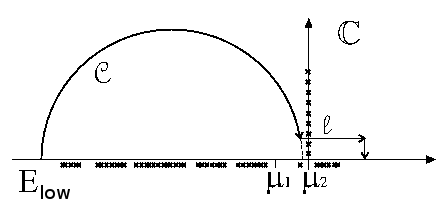
\includegraphics[width=8.0cm]{Fig_integration.png}
\caption{ \label{fig:contour} Contour integration in the complex plane for the
  Green's fuctions. The crosses represent poles of either $G^r$ or the Fermi
  function.}
\end{center}
\end{figure}
All integrations are performed with Gaussian quadratures and the number of
points must be specified manually. The complex contour integration is subdivided
into two sections: the first section is an arc of circle, $\mathcal{C}$, that
can be computed with few integration points (default 20); the second section is
a line that intersects the contour and runs parallel to the real axis at a
distance that depends on the number of poles of the Fermi function enclosed
within the contour. Usually a good choice for the number of poles is between 3
and 5 (the default is 3). The poles are placed at the complex points $z_m = E_F
+ i (2m+1) \pi k T$ and, therefore, are separated from each other by $2 \pi k
T$.  At $T=300$~K this corresponds to a separation of 156~meV. It should be
noted that, as the temperature decreases, the separation between poles
reduces. This makes the contour integration harder as it needs to walk across
two singularities. At very low temperatures, $T=10$~K, the separation is 5.2
meV. Below this temperature the contour integration is treated as $T=0$ in order
to avoid numerical inaccuracies. The integration along the segment $\mathcal{L}$
extends up to $Re\left[ z \right]=E_F+nkT$, where $n$ is an integer number
specified by the keyword \kw{FermiCutoff} and has a default value of 10.  In the
limit $T=0$~K the poles collapse into a non-analytic cut and the contour needs
to be changed such that the second section of the complex contour becomes the
arc of circle closing on the real axis.  Finally, the real axis integration
extends between the lowest and highest chemical potentials. The number of
quadrature points should depend on the bias itself and can be set using
\kw{RealAxisPoints} or \kw{RealAxisStep}. The default value is
$1\text{~pt}/0.018\text{~eV}$ (actually $1500\text{~pt}/1\text{~H}$). In finite
temperature calculations the segment is extended to include the Fermi cutoff by
$nkT$ on both sides ($\mu_1-nkT, \mu_2+nkT$). In this case the number of
quadrature points are increased by assuming the same point density defined in
the range ($\mu_1, \mu_2$).  Example: for a bias of 0.2 V, the default number of
points is $0.2\cdot1500/27.21139=11$. At $T=300$~K the interval is increased by
0.26~eV on both sides, therefore $0.26\cdot1500/27.21139=14.33$ which is
truncated to 14 points, leading to a total of 38 points along the real axis. The
use of the keyword \kw{RealAxisStep} is usually more convenient because it
ensures a consistent real axis integrations during, for example, a bias sweep.

Note: The GF solver can be used also for calculations other than the transport
context. In case the position of the Fermi Energy is known with good accuracy
the density matrix solver based on the GF can be used to compute the electronic
properties of clusters and supercells. The recursive algorithm may be an
efficient solution to large problem and could be efficient for systems having an
elongated 1D shape.

\section{Poisson solver}

The Poisson solver can not be used at the moment together with Model NoGeometry calculations
and is not used for Non-SCC calculations, but it
is a fundamental part of the non-equilibrium SCC transport
calculations and must be declared whenever a NEGF calculation is performed using
\is{Electrostatics = Poisson}. Under non-equilibrium conditions the
self-consitent potential of the KS equations cannot be solved using the
efficient $\gamma$-functional, but requires the definition of appropiate
boundary conditions for the potentials imposed on the contacts. However, since
the $\gamma$-functional is formally identical to a pure Hartree potential, it
can be obtained in real space by solving a Poisson solver.  The Poisson equation
is solved in a {\em box} with hexahedral prism shape. This restriction is
imposed by the solver employed. This restricts calculations of supercell
structures to orthorhombic super-lattices.  An additional restriction is that
the box sides must be aligned with the Cartesian axes, x, y, z.

\begin{ptableh}
  \kw{PoissonBox} & 3r & &  &  \\
  \kw{MinimalGrid} & 3r  &  & 0.5 0.5 0.5 & \\
  \kw{PoissonAccuracy} & r &  & 1e-7 &  \\
  \kw{AtomDensityTolerance}  & r  &  & 1e-6 & \\
  \kw{CutoffCheck} & l & & Yes & \\
  \kw{Verbosity} & i & & 51 & \\
  \kw{SavePotential} & l & & No & \\
  \kw{PoissonAccuracy} & r & & 1e-6 & \\
  \kw{MaxPoissonIterations} & i & & 60 & \\
  \kw{BuildBulkPotential} & l & & Yes & \pref{Boundary Conditions}\\
  \kw{ReadOldBulkPotential} & l & & Yes & \pref{Boundary Conditions} \\
  \kw{OverrideDefaultBC} & m & & none\{\} & \pref{Boundary Conditions}\\
  \kw{OverrideBulkBC} & m & & none\{\} & \pref{Boundary Conditions}\\ 
  \kw{BoundaryRegion} & m & & global\{\} &  \pref{Boundary Conditions} \\
  \kw{Gate} & m & & none\{\} & \pref{Electrostatic Gates} \\ 
  \kw{MaxParallelNodes} & m & & none\{\} & \pref{Parallelizations} \\ 
\end{ptableh}



\begin{description}
\item[\is{PoissonBox}]\modif{\modtype{length}} Dimension of the Poisson box
  along directions x, y and z.
\item[\is{MinimalGrid}]\modif{\modtype{length}} The minimal requested grid
  spacing along x, y and z. The actual grid spacing chosen by the multigrid will
  be lower than this.  charge densities.
  \item[\is{AtomDensityTolerance}] In order to calculate the potential, the
    Mulliken charges are projected on the real space grid. This parameter
    defines the cutoff after which the charge is considered vanish (i.e., the
    space extension of the projected charge). The default is 1e-6. Note that the
    contacts must be at least twice the length of the extent of a projected
    Mulliken charge. If this conditions is not fullfilled and is set to Yes, the
    code will exit with an error message. Setting this parameter to a lower
    value could allow to define shorter contacts in some cases. However this
    could lead to relevant error in the potential hence to spurious reflections,
    therefore it should be left to default value or changed very carefully.
  \item[\is{CutoffCheck}] If set to No, consistency between contact length and
    charge extension is not verified (see above section). The default is No. As
    for AtomDensityTolerance, this parameter shouldn't be touched unless you
    know exactly what you're doing.
  \item[\is{Verbosity}] This parameter controls the amount of output messages
    and takes values ranging from 1 to 100.
  \item[\is{SavePotential}] Save the potential to file. 
\item[\is{PoissonAccuracy}] Defines the accuracy for the approximate solution of
  the Poisson equation (default value 10$^{-6}$).
\item[\is{MaxPoissonIterations}] Defines the maximum amounts of iterations for
  the solver.
\end{description}

{\bf Note}: The Poisson Box can be specified using the keyword
\verb|PoissonBox|. In calculations in which the two contacts face each other
along the same axis, setting the box-size along this axis has no effect because
the code needs to adjust the correct size internally.  This keyword is redundant
(and should not be specified) when the system is periodic, since in this case
the Poisson box is taken from the supercell lattice vectors.

Numerical error in the potential will results in spurious discontinuities at the
contact-device interfaces. The default tolerances should do the job in most
cases.

This is a tipical example of the whole Poisson block specification. Some of the
keywords are described in the next subsections.


Example:
 
\begin{verbatim}
 Electrostatics = Poisson {
  PoissonBox [Angstrom] = 20.0 20.0 20.0
  MinimalGrid [Angstrom] = 0.3 0.3 0.3
  SavePotential = No
  BuildBulkPotential = Yes
  ReadOldBulkPotential = No
  BoundaryRegion = Global {}
  PoissonAccuracy = 1e-7
  Gate = Planar{
      GateLength_l [Angstrom] = 10.0
      GateLength_t [Angstrom] = 20.0
      GateDistance [Angstrom] = 7.0
      GatePotential [eV] = 1.0
  }
}
\end{verbatim}

\subsection{Boundary Conditions}
\label{Boundary Conditions}

The Poisson equation is solved imposing special boundary conditions (BC) on the
six faces of the Poisson Box. In basic transport calculations, comprising two
contacts placed along the same axis, the BCs are choosen as follows:

\begin{description}
\item[Dirichlet] Fixed potentials on the two contact faces with values defined
  by the applied potentials (see \is{UploadContacts}, \is{ContactPotentials}).
\item[Neumann] Zero normal field on the remaining 4 lateral box faces.
\end{description}
In periodic supercells the BCs are: {\bf Dirichlet} (fixed potentials) on the
two contact faces with values defined by the applied potentials (see
\is{UploadContacts}, \is{ContactPotentials}) and {\bf Periodic} on the remaining
4 lateral box faces.

In some specific cases Neumann BCs can be set on one contact. In order to do so
it is necessary to use \verb|OverrideDefaultBC| (see below).

Device and contact potentials should smoothy join at the interface. In order to
reach this goal the code computes the Bulk potential of each contact and uses
the result as a BC on the contact face of the Poisson box. This is useful when
the contact potential is not uniform due to charge rearrangments. The external
applied contact potential is added to the bulk potential.  The user can
deactivate this calculation with the keyword \kw{BuildBulkPotential}.

{\bf Note}: The bulk potential is computed on a special box that has 'lateral'
sizes copied from the device box, and has the size of one PL along the contact
direction. The BCs are --so to speak-- inherited from the device region. In
particular:
\begin{enumerate}
\item Along the contact direction periodic BCs are imposed.
\item On the other four faces the BCs are copied from the device region.
\item The user can override this setting using \verb|OverrideBulkBC| (see
  below).
\item When all four faces inherit Neumann BC (default for the device region),
  these are ALL internally changed to Dirichlet, because the solver cannot
  handle this situation that gives rise to a singular matrix.
\end{enumerate}

\begin{description}
\item[\is{BuildBulkPotential}] (default: \is{Yes}) is used to calculate the
  electrostatic potential of the contacts and the result is used as a Dirichlet
  boundary condition on the contact face (superimposed to the contact
  potential).
\item[\is{ReadOldBulkPotential}] Read a previously computed bulk potential from
  hard-disk.
\item[\is{BoundaryRegion}] Specifies how the Dirichlet boundary conditions are
  treated on each contact face of the Poisson box. It can be \kw{Global},
  \kw{Square} or \kw{Circle}. \kw{Global} means that the BC is applied to the
  entire face of the box, whereas the other keywords imply that the Dirichlet
  BC are applied on a cross-section projected on the contact face. This is
  useful for instance when handling nanowire contacts, for which it is not
  really consistent to impose a constant potential on the whole face of the
  Poisson box.
\item[\is{BufferLength}]\modif{\modtype{length}} can be used to set the size of
  the boundary region beyond the atomistic size which is determined as the
  minimal circle or qquare containg all atoms of the contact cross-section.
\end{description}

Example:
\begin{verbatim} 
BoundaryRegion = Circle {
    BufferLength [Angstrom] = 3.0 
}  
\end{verbatim}

In some special case it might be necessary to override the default BCs applied
by the code on the Poisson equation. Currently this can be done using the
keywords: \verb|OverrideDefaultBC| and \verb|OverrideBulkBC|.

\begin{description}
\item[\is{OverrideDefaultBC}] block is used to override the BCs described
  above. It can be used to force Dirichlet or Neumann BCs along some specified
  directions or on one of the four lateral faces of the Poisson box.
\item[\is{Boundaries}] is used to specify on which face different BCs must be
  imposed. Assuming contacts along z, the keyword can be set any of xmin, xmax,
  x, ymin, ymax, y.
\end{description}

\begin{verbatim}
OverrideDefaultBC = Dirichlet {
      Boundaries = xmin   
}
\end{verbatim}

For instance setting Dirichlet BC on \verb|Boundaries = xmin| imposes
$\phi(x,y,z)=0$ on the face placed at $x=x_{\text{min}}$,
\verb|boundaries = xmax| imposes $\phi(x,y,z)=0$ on the face placed at
$x=x_{\text{max}}$. When Dirichlet needs to be forced on both faces, it is
possible to use either \verb|boundaries = xmin,xmax| or simply
\verb|boundaries = x|. The same syntax can be used to impose conditions on more
faces, using \verb|boundaries = x,y| or \verb|boundaries = x,ymin|.

A similar strategy can be used to impose different boundary conditions on the
contacts. For instance, a Neumann BC can be set on one contact face using

\begin{verbatim}
OverrideDefaultBC = Neumann {
      Boundaries = zmin   
}
\end{verbatim}

{\bf Note} that the user should know which face of the Poisson Box corresponds
to the desired contact. Furthermore, if the user sets Neumann at all contacts
the Poisson solver will not converge (singular matrix) unless Dirichlet is
imposed somewhere else (e.g., a gate potential is present).

It is also possible to override default BCs when computing the bulk potential.

\begin{description}
\item[\is{OverrideBulkBC}] block is used to override bulk BC usually copied from
  the device region.
\item[\is{Boundaries}] has the same meaning and syntax as in
  \verb|OverrideDefaultBC|.
\end{description}


\begin{verbatim}
OverrideBulkBC = Neumann {
      Boundaries = x, y   
}
\end{verbatim}



\subsection{Electrostatic Gates}
\label{Electrostatic Gates}

The option \kw{Gate} can be used to specify an electrostatic gate. Currently the
gate type \kw{Planar} and \kw{Cylindrical} are allowed.  Restrictions. The
planar gate must be placed with its face parallel to the x-z plane, i.e., the
gate direction must be along y. At the same time the transport direction should
be placed along the z-axis. The latter is not really a restriction but it gives
meaning to 'longitudinal' and 'transverse' in the geometrical definitions of the
gate lengths.  Example:

\begin{verbatim} 
Gate = Planar {
    GateLength_l [Angstrom] = 20.0
    GateLength_t [Angstrom] = 20.0
    GateDistance [Angstrom] = 7.0
    GatePotential [eV] = 1.0
}

Gate = Cylindrical {
    GateLength [Angstrom] = 10.0
    GateRadius [Angstrom] = 7.0
    GatePotential [eV] = 1.0
}
\end{verbatim}

%<<<<<<< HEAD
The various options for the gates have the following meanings:
\begin{description}
\item[\is{GateLength\_l}]\modif{\modtype{length}} Sets the gate length along the
  transport direction (assumed to be z). The gate is centered in the device
  region.
\item[\is{GateLength\_t}]\modif{\modtype{length}} Sets the gate transverse to
  the transport direction (assumed to be x). The gate is centered in the device
  region.
\item[\is{GateDistance}]\modif{\modtype{length}} Sets the distance of the gate
  from the center axis of the device region.
\item[\is{GatePotential}]\modif{\modtype{energy}} Sets the potential applied to
  the gate.
\item[\is{GateRadius}]\modif{\modtype{length}} For cylindrical gate, sets the
  distance of the gate from the center axis or gate radius.
%\item[\is{InsulatorLength}]\modif{\modtype{length}} For cylindrical gate, sets
%  the insulator length.
%\item[\is{InsulatorRadius}]\modif{\modtype{length}} For cylindrical gate, sets
%  the insulator radius (smaller than the GateRadius).
%\item[\is{TransitionLength}]\modif{\modtype{length}} Sets the length of a
%  transition (buffer) region between the dielectric insulator and vacuum
%  ($\kappa=1$).
%\item[\is{Kappa}] Sets the insulators relative dielectric constant ($\kappa$).
\end{description}
%=======
%The variable type is real, complex, integer or logical. The shape information is
%\newline :ndim: size$_1$,size$_2$,$\ldots$,size$_{ndim}$:\newline where ndim is
%the number of dimensions, organised with the Fortran convention and of size
%size$_1$ $\times$size$_2$ $\times$size$_2$ $\times \ldots$.
%>>>>>>> dftbplus_git

Note that the gate option has not be tested tharoughly and may still contain
bugs.  Please report to the developers any problem encountered.

Developments. In forthcoming releases also double gates will be possible.
Similarly to a usual \dftbp{} calculation, the output from a Transport calculation
will be generated in the \verb|detailed.out| and \verb|detailed.xml|. These
files are self-documenting, i.e. you will find a human-readable description of
the output data in the files themselves. After a transport calculation, the
files will contain the transmission coefficient for every energy point and for
every k point and the local density of states for every energy point and
projection ranges specified in input. They will also contain the total current
and the partial current for every k point. In multiterminal calculation, this
data will be written for every terminal couple.

{\new

\section{Model Hamiltonians} 
\label{sec_model}

To use the external Hamiltonian without geometry \big(if \is{Geometry = NoGeometry\{\}}\big), the type of the Hamiltonian must be set to \iscb{Model}:
%
\begin{verbatim}
Hamiltonian = Model{}
\end{verbatim}

The \iscb{Model} method may contain the
following properties:

\begin{ptableh}
  \kw{NumStates} & i &  & No default!  & \\
  \kw{HamiltonianFile} & s &  & H.mtr & \\
 
  \hline
\end{ptableh}

\begin{description}
  \item[\is{NumStates}] Is a full number of states in the Hamiltonian. Required for model calculations without geometry. 

  \item[\is{HamiltonianFile}]\modif{\modtype{energy}} The name of the data file with the Hamiltonian, saved as an array of real numbers. 
    
\end{description}

Model Hamiltonians are used at the moment only for transport calculations. It is important to add the property \iscb{ContactPLs} to the \iscb{Device} section (see Sec.\,\ref{sec_device}). 

\section{Elastic dephasing}
\label{sec_deph}

To switch on the dephasing effects, the group \iscb{Dephasing} must be included into the Hamiltonian group.
The \iscb{Dephasing} group may contain the following methods/properties:

\begin{ptableh}
  \kw{BuettikerProbes} & m &  & none\{\}  & \\
  \kw{VibronicElastic} & m &  & none\{\}  & \\
  
  \hline
\end{ptableh}

\subsection{B\"uttiker probes}

\begin{description}
  
\item[\is{BuettikerProbes}] switches on the B\"uttiker probe dephasing. There are two methods: \iscb{ZeroPotential} and \iscb{ZeroCurrent}. The first one describes physical conducting environment with fixed (at the moment zero) electrical potential. The second is for the {\it B\"uttiker Probe Model} of dephasing, when the zero-current condition is fulfilled by artificial adjustment of local electrical potentials.

\begin{verbatim}   
BuettikerProbes = ZeroPotential {
  Coupling [eV] = constant { 0.01 }
}

BuettikerProbes = ZeroCurrent {
  Coupling [eV] = constant { 0.01 }
}
\end{verbatim}

\end{description}  

\begin{description}
\item[\is{Coupling}]\modif{\modtype{energy}} describes coupling to the environment. The method \iscb{constant} couples all states equivalently. The other possible methods are \iscb{AtomCoupling} -- with different couplings for different atoms, and \iscb{AllOrbitals} -- with different couplings for all atomic orbitals. For the model calculations these two options are equivalent. 

\begin{verbatim}   
Coupling [eV] = AtomCoupling {
  AtomList { Atoms = 1
             Value = 0.1
  }
  AtomList { Atoms = 2 3
             Value = 0.01
  }
  AtomList { Atoms = 4 5
             Value = 0.03
  }
}

Coupling [eV] = AllOrbitals { 0.1 0.1 0.1 ... }
\end{verbatim}

\end{description}  
  
\subsection{Vibronic dephasing}

\begin{description}

\item[\is{VibronicElastic}] switches on the elastic vibronic dephasing method. There is only one method \iscb{local} available at the moment. The \iscb{Coupling} method can get the same values as for B\"uttiker probe dephasing. There are several additional options: 
\is{AtomBlock} (default=.false.), which changes the way of coupling between electrons and phonons; \is{MaxNumIter} -- the maximum number of iterations (default=100); \is{Mixing} -- control of mixing in the self-consistent cycle (default = 0.05); \is{Tolerance} -- control of the convergency tolerance (default = 0.001). 
  
\begin{verbatim}
VibronicElastic = local {
  AtomBlock = Yes
  Coupling [eV] = Constant {0.01}
  MaxNumIter = 1000
  Mixing = 0.5
  Tolerance = 0.001
}
\end{verbatim}
  
\end{description}

\section{Application to STM spectroscopy}
\label{sec_stm}


} %end of \new

\section{Parallelizations}
\label{Parallelizations}

The code has been parallelised in two main parts. The Non-equilibrium Green's
functions are computed by distributing the energy points along the countour and
real axis calculations. Contour and real axis integrations are independent and
separately distributed. Load balancing has to be taken care by the user. For
instance if ContourPoints = \{20 20\} and RealAxisPoints = 60, by setting 10 MPI
nodes, each node will handle 4 points along the contour and 6 points along the
real axis.

Mixed OpenMP/MPI calculations are possible. When compiling dftb+ the user should
link against threaded mkl, rather than sequential. Numerical experiments show
that best performance on multicore CPUs is generally obtained by running
independent MPI processes on physical sockets, exploiting OpenMP multithreading
on each socket. For instance NEGF can exploit threaded matrix-matrix
products. The user can experiment by setting the environment variable
OMP\_NUM\_THREADS.

The Poisson solver has not been parallelized yet. However the efficient
multigrid solver does not typically represent a bottleneck. Currently the
assembly of the charge density on the real-space grid and the projection of the
potential on the atoms have been parallelized. Since gather of the charge
density on each node can easily hit communication bottlenecks the user can use
the parameter \kw{MaxParallelNodes} to control distributions of these
calculations. The default is \kw{MaxParallelNodes}=1, that can be increased
until speedups are observed.
\begin{ptable}
 \kw{MaxParallelNodes} & i & & 1 &  \\ 
\end{ptable}


\section{Analysis}

The \kw{Analyis} block is used to specify post-scf calculations such as
tunneling or projected DOS.

\begin{verbatim} 
Analysis{
  TunnelingAndDOS{
    EnergyRange [eV] = {-5.0 -3.0}
    EnergyStep [eV] = 0.02    
  }
}
\end{verbatim}


\htsection{TunnelingAndDos}

This method block can be specified in \iscb{Analysis} and it is
used to calculate the transmission by means of Caroli formula, the current by
means of Landauer formula and the Density of States from the spectral
function. This block can only be specified if an open boundary system has been
defined in \iscb{Transport}.
 
\begin{ptable}
  \kw{EnergyRange} & 2r &  & &  \\
  \kw{EnergyStep} & r & &  &  \\
  \kw{TerminalCurrents} &p& & & \\
  \kw{Region} & p & & & \pref{Region} \\
  \kw{WriteTunn} & l & & Yes & \\
  \kw{WriteLDOS} & l & & Yes & \\
  \hline
\end{ptable}


\begin{description}


\item[\is{EnergyRange}]\modif{\modtype{energy}} Contains the energy range over
  which the transmission function and local density of states are computed.
\item[\is{EnergyStep}]\modif{\modtype{energy}} Is the energy sampling step.
\item[\iscb{TerminalCurrents}] in multiterminal configurations is used to define
  the terminal across which current must be computed. The terminal pairs are
  defined by using the keyword \is{EmitterCollector}. example:
  
   \begin{verbatim}
    TerminalCurrents{
       EmitterCollector = {"source" "drain"}
       EmitterCollector = {"source" "gate"}
    }
  \end{verbatim}   
  
  The block \is{TerminalCurrents} may be omitted since the code automatically
  sets all possible independent combinations for the terminal currents. For
  example in a 4-contact calculations the currents are 1-2, 1-3, 1-4, 2-3, 2-4,
  3-4.
\item[\iscb{Region}] \label{Region} This block defines atomic ranges or orbitals
  where the local density of states is calculated projected. The definition in
  the block follow the same syntax as a \dftbp{} calculation without transport.
\item[\is{WriteTunn}] The transmission coefficients are written also to a
  separate file for quick reference. If set to No, the transmission coefficient
  are only written to \dftbp{} output files (detailed.out and detailed.xml,
  autotest.tag).
\item[\is{WriteLDOS}] same as above, for the density of states.

\end{description}


\section{Troubleshooting}

\dftbp{} transport machinery is designed to calculate transport in structures
with a large number of atoms. To take full advantage of the iterative algorithm,
be sure that the system is correclty partitioned in Principal Layers, as
described in Transport and Green's solver sections. Be aware that a wrong
partitioning will lead to wrong results. If you're not completely confident, you
can run a calculation on a test system with and without partitioning. The
results should be the same.

On some systems, a \verb|Segmentation Fault| error could occur while running
relatively large structures. This could happen because the stack memory limit
has been exceeded. You can troubleshoot this setting a higher limit for the
stack memory. In bash you can remove stack memory limitation with the command
line \verb|ulimit -s unlimited|.


\chapter{Output of \dftbp}
\label{sec:dftbp.output}

This chapter contains the description of some of the output files of
\dftbp{} where the output format is not self documenting. Unless
indicated otherwise, numbers in the output files are given in atomic
units (with Hartree as the energy unit).

\section{hamsqrN.dat, oversqr.dat}
\label{sec:dftbp.hamsqr}
\index{hamsqr.dat}\index{oversqr.dat}

The files \verb|hamsqrN.dat| and \verb|oversqr.dat| contain the square
(folded) Hamiltonian and overlap matrices. The number \verb|N| in the
filename \verb|hamrealN.dat| indicates the spin channel. For spin
unpolarised calculation it is 1, for spin polarised calculation it is
1 and 2 for spin-up and spin-down, respectively while for non-collinear
spin it is charge, $x$, $y$ and $z$ for 1, 2, 3 and 4. Spin orbit is
not currently supported for this option.

Only non-comment lines (lines not starting with "\#") are documented:
\begin{itemize}

\item Flag for signalling if matrix is real (\verb|REAL|), number of
  orbitals in the system (\verb|NALLORB|), number of kpoints
  (\verb|NKPOINT|). For non-periodic (cluster) calculations, the
  number of kpoints is set to 1.

\item For every $k$-point:
  \begin{itemize}
  \item Number of the $k$-point. For molecular (non-periodic)
    calculations only 1 $k$-point is printed.
  \item The folded matrix for the given $k$-point. It consists of
    \verb|NALLORB| lines $\times$ \verb|NALLORB| columns. If the
    matrix is not complex (\verb|REAL| is \verb|F|), every column
    contains two numbers (real and imaginary part).
  \end{itemize}
\end{itemize}

The files are produced if requested by \is{WriteHS} = \is{Yes} (see
section~\ref{kw:dftbp.WriteHS}).

\section{hamrealN.dat, overreal.dat}
\label{sec:hamreal}
\index{hamreal.dat}\index{overreal.dat} The files \verb|hamrealN.dat|
and \verb|overreal.dat| contain the real space Hamiltonian and overlap
matrices. The number \verb|N| in the filename \verb|hamrealN.dat|
indicates the spin channel. For spin unpolarised calculation it is 1,
for spin polarised calculation it is 1 and 2 for spin-up and
spin-down, respectively, while for non-collinear spin it is charge,
$x$, $y$ and $z$ for 1, 2, 3 and 4. Spin orbit is not currently
supported for this option.

Note: The sparse format contains only the "lower triangle" of the real
space matrix. For more details about the format and how to obtain the
upper triangle elements, see reference~\cite{dftbp-paper}. Also note,
that for periodic systems the sparse format is based on the
\emph{folded} coordinates of the atoms, resulting in translation
vectors (ICELL) which look surprising at first glance.

Only non-comment lines (lines not starting with "\#") are documented:
\begin{itemize}
\item Number of atoms in the system (\verb|NATOM|)
\item For every atom:
  \begin{itemize}
  \item Atom number (\verb|IATOM|), number of neighbours including the
    atom itself (\verb|NNEIGH|), number of orbitals on the atom
    (\verb|NORB|)
  \end{itemize}
\item For every neighbour of every atom:
  \begin{itemize}
  \item Atom number (\verb|IATOM1|), neighbour number (\verb|INEIGH|),
    corresponding image atom to the neighbour in the central cell
    (\verb|IATOM2F|), coefficients of the translation vector between
    the neighbour and its corresponding image (\verb|ICELL(1)|,
    \verb|ICELL(2)|, \verb|ICELL(3)|). Between the coordinates of the
    neighbour $\mathbf{r}_{\text{INEIGH}}$ and the image atom
    $\mathbf{r}_{\text{IATOM2F}}$ the relation
    \begin{equation*}
      \mathbf{r}_{\text{INEIGH}} = \mathbf{r}_{\text{IATOM2F}} + \sum_{i=1}^3
      \text{ICELL}(i)\, \mathbf{a}_i
    \end{equation*}
    holds, where $\mathbf{a}_i$ are the lattice vectors of the supercell.
  \item The corresponding part of the sparse matrix. The data block
    consists of \verb|NORB(IAT1)| lines and \verb|NORB(IAT2F)| columns.
  \end{itemize}
\end{itemize}

The files are produced if requested by \is{WriteRealHS} = \is{Yes}
(see section~\ref{kw:dftbp.WriteRealHS}).

\section{eigenvec.out, eigenvec.bin}
\label{sec:dftbp.eigenvec}
\index{eigenvec.out}\index{eigenvec.bin}

These files contain the eigenvectors from the Hamiltonian, stored
either as plain text (eigenvec.out) or in the native binary format of
your system (eigenvec.bin).

The plain text format file \verb|eigenvec.out| contains a list of the values of
the components of each eigenvector for the basis functions of each atom. The
atom number in the geometry, its chemical type and the particular basis function
are listed, followed by the relevant value from the current eigenvector and then
the Mulliken population for that basis function for that level\index{state
  resolved Mulliken population}. The particular eigenvector, $k$-point and spin
channel are listed at the start of each set of eigenvector data. In the case of
non-collinear spin, the format is generalised for spinor wavefunctions. Complex
coefficients for both the up and down parts of the spinors are given (instead of
single eigenvector coefficient) followed by four values -- total charge, then
$(x,y,z)$ magnetisation.

The binary format file \verb|eigenvec.bin| contains the (unique) runId of the
DFTB+ simulation which produced the output followed by the values of the
eigenvectors. The eigenvector data is ordered so that the individual components
of the current eigenvector are stored, with subsequent eigenvectors for that
$k$-point following sequentially. All $k$-points for the current spin channel
are printed in this order, followed by the data for a second channel if spin
polarised.

The files are produced if requested by setting \is{WriteEigenvectors} =
\is{Yes}, with \is{EigenvectorsAsTxt} being also required to produce the plain
text file (see section~\ref{kw:dftbp.WriteEigenvectors} for details).

\section{charges.bin}
\label{sec:charges.bin}
\index{charges.bin}

The file charges.bin contains the orbitally-resolved charges for each atom,
ordered as the charges on each orbital of an atom for a given spin channel, then
each spin channel and finally over each atom. In later versions of \dftbp{} this
format includes a check sum for the total charge and magnetisation. In the case
of orbital potentials (p.~\pref{sec:DFTB+U}) the file also contains extra
population information for the occupation matrices.

This file is produced as part of the mechanism to restart SCC calculations, see
sections~\ref{kw:dftbp.RestartFrequency} and~\ref{kw:dftbp.MDRestartFrequency}.

\section{md.out}
\label{sec:md.out}
\index{md.out}

This file is only produced for \iscb{VelocityVerlet} calculations (See
p.~\pref{sec:dftbp.VelocityVerlet}). It contains a log of information generated during MD
calculations, and appended every \kw{MDRestartFrequency} steps. In the case of
small numbers of atoms and long MD simulations it may be useful to set
\is{WriteDetailedOut} to \is{No} and examine the information stored in this file
instead.

\section{Excited state results files}
\label{sec:tddftb_lr}
Several files are produced during excited state calculations depending on the
particular settings from section~\ref{sec:dftbp.ExcitedState}.

\textbf{Note:} in the case of degeneracies, the oscillator strengths depend on
arbitrary phase choices made by the ground state eigensolver. Only the sum over
the degenerate contributions is well defined for most single particle transition
properties, and label ordering of states may change if changing eigensolver or
platform. For the excited state, properties like the intensities for
individual excitations in degenerate manifolds again depend on phase choices
made by both the ground and excited eigensolvers.


\subsection{ARPACK.DAT}
\index{ARPACK.DAT}

Internal details of the ARPACK solution vectors, see the ARPACK
documentation~\cite{Lehoucq97arpackusers} for details.

\subsection{COEF.DAT}
\index{COEF.DAT}

Data on the projection of this specific excited state onto the ground state
orbitals. For the specific exited state, the (complex) decomposition of its
single particle states onto the ground state single particle levels, together
with its fractional contribution to the full excited state are given.

General format:

\begin{tabular}{|l|p{5.5cm}|}
\hline
{\small T F                                }&Legacy flags\\
{\small   1  1.9999926523  2.0000000000    }&level 1, fraction of total WF, 2.0\\
{\small-0.1944475716  0.0000000000 -0.1196876988  0.0000000000 ....    }&real then
imaginary projection of level 1\\
                                    &onto ground state 1, then ground state 2, etc.\\
{\small-0.1196876988  0.0000000000 -0.1944475703  0.0000000000 ....    }&\\
{\small.}&\\
{\small.}&\\
{\small.}&\\
{\small   2  1.9999866161  2.0000000000    }&level 2\\
{\small-0.2400145188  0.0000000000 -0.1767827333  0.0000000000 ....}& real then
imaginary projection of state 2\\
{\small.}&\\
{\small.}&\\
{\small.}&\\ \hline
\end{tabular}

\subsection{EXC.DAT}
\index{EXC.DAT}

Excitations data including the energies, oscillator strength, dominant Kohn-Sham
transitions and the symmetry.

Example first few transitions for C$_4$H$_4$:

\begin{verbatim}
     w [eV]       Osc.Str.         Transition         Weight      KS [eV]    Sym.

 =========================================

      5.551       0.5143882       11   ->    12        1.000       4.207      S
      5.592       0.0000000       10   ->    12        1.000       5.592      S
\end{verbatim}

Two examples of singlet transitions with energies of 5.551 and 5.592~eV. The
first is dipole allowed, the second not. In both cases they are transitions
primarily (weight of 1.000) to single particle state 12, and are of singlet
character (``S'').

In the case of spin-polarised calculations, an additional column of values are
given instead of the symmetry, showing the level of spin contamination in the
state (labelled as \verb|D<S*S>|), with typically states where a magnitude of
less than 0.5 is usually considered reliable~\cite{garcia14Thesis}.

\subsection{SPX.DAT}
\index{SPX.DAT}

Single particle excitations (SPX) for transitions between filled and empty single
particle states of the ground state. These are given in increasing single
particle energy and show the oscillator strength and index of the Kohn-Sham-like
states that are involved.

\begin{verbatim}
       #      w [eV]       Osc.Str.        Transition

 ============================

       1      5.403       0.2337689       15   ->    16  
       2      5.403       0.2337689       14   ->    16  
       3      5.403       0.2337689       15   ->    17  
       4      5.403       0.2337689       14   ->    17  
       5      6.531       0.0000000       13   ->    16  
       6      6.531       0.0000000       12   ->    16  
\end{verbatim}

\subsection{TDP.DAT}
\index{TDP.DAT}

Detail of the magnitude and direction of the transition dipole from the ground
to excited states.

\subsection{TRA.DAT}
\index{TRA.DAT}

Decomposition of the transition from the ground state to the excited states. The
energy and spin symmetry are given together with the contributions from each of
the single particle transitions.

\subsection{TEST\_ARPACK.DAT}
\index{TEST\_ARPACK.DAT}

Tests on the quality of the eigenvalues and vectors returned by ARPACK. For the
$i^\mathrm{th}$ eigen-pair, the eigenvalue deviation corresponds to the
deviation from $\left( \langle \mathbf{x}_i | H | \mathbf{x}_i\rangle -
\epsilon_i \right)$, The eigen-vector deviation is a measure of rotation of the
vector under the action of the matrix: $\left| \left( H | \mathbf{x}_i\rangle -
\epsilon_i | \mathbf{x}_i\rangle \right) \right|_2$, the normalisation deviation
is $\langle \mathbf{x}_i | \mathbf{x}_i\rangle - 1$ and finally largest failure
in orthogonality to other eigenvectors is given.

Example:\\
\begin{tabular}{lllll}
{\tt State} & {\tt Ei deviation} & {\tt Evec deviation} & {\tt Norm deviation} &
{\tt Max non-orthog}\\ {\tt 1} & {\tt -0.19428903E-15} & {\tt 0.80601119E-15} &
{\tt 0.19984014E-14} & {\tt 0.95562226E-15}\\ {\tt 2} & {\tt 0.27755576E-16} &
{\tt 0.85748374E-15} & {\tt 0.48849813E-14} & {\tt 0.36924443E-15}\\ {\tt 3} &
{\tt -0.12490009E-15} & {\tt 0.88607302E-15} & {\tt 0.88817842E-15} & {\tt
  0.60384195E-15}\\
\end{tabular}

\subsection{XCH.DAT}
\index{XCH.DAT}

Net charges on atoms in the specified excited state. The top line contains the
symmetry (Singlet or Triplet) and the number of the excited state. The next line
is the number of atoms in the structure followed by some header text. Then on
subsequent lines the number of each atom in the structure and its net charge are
printed.

\subsection{XplusY.DAT}
\index{XplusY.DAT}

Expert file with the RPA  $(X+Y)^{I\Sigma}_{ia}$ data for all the calculated
excited states.

Line 1: number of single particle excitations and the number of calculated
excited states\\
Line 2: Level number 1, nature of the state (S, T, U or D) then excitation
energy (in Hartree)\\
Line 3: expansion in the KS single particle transitions\\
.\\
.\\
.\\
Line 2: Level number 2, nature of the state (S, T, U or D) then excitation
energy (in Hartree)\\

\subsection{XREST.DAT}
\index{XREST.DAT}

Net dipole moment of the specified excited state in units of Debye.

%%% Local Variables: 
%%% mode: latex
%%% TeX-master: "manual"
%%% End: 

\chapter{Transport calculations}
\label{app:transp}

Within {\dftbp} it is possible to treat quantum mechanical
systems with open boundary conditions, i.e.\ systems connected to external
reservoirs and therefore quantum transport.  A new specific \kwcb{Transport}
block has been added to specify the geometry of such transport problems.
Additional solvers have been added to the \kw{Eigensolver} section to either
fully solve the open boundary problem (using the keyword \kwcb{GreensFunction})
or the transmission through the system (\kw{TransportOnly}). Finally a
real-space Poisson solver is available for self consistent charge calculations
and electrostatic gates (within a new section, \kw{Electrostatics}, using the
keyword \kwcb{Poisson}).

\section{Definition of the geometry}
\label{sec:transport.geometry}

The input geometry for transport calculations can be a little tricky. In
comparison to cluster or supercell boundary conditions, the geometry for
transport calculation must also contain information about the contacts (external
reservoirs). The contacting leads (or surfaces) are actually semi-infinite
structures, supporting travelling waves. Unlike finite structures, where no
stationary current is possible, travelling waves can only exist in such open
systems.  The simulation is therefore partitioned into a device region and two
or more contact regions.

Rules to build a valid input structure:
\begin{enumerate}
\item \label{rule1} All device atoms must come first in the structure.
\item \label{rule2} Each contact must comprise of two subsequent unit cells,
  called principal layers (PLs). The two PLs together give all information about
  the contact structure and in the following are referred generally as a
  ``contact''.
\item \label{rule3} A PL is a unit cell of the contacting lead that has
  interactions only with its nearest neighbour PLs in tight-binding terms
  (i.e.\ the Slater-Koster interactions only extend into immediately neighbouring
  PLs).
\item \label{rule4} The ordering of the atoms within the two PLs of a contact
  must be consistent, in the sense that the two PLs must be exact periodic
  replicas of each other: If each PL comprise $N$ atoms, the $i^\mathrm{th}$
  atom in the first PL must have a corresponding identical atom, $i+N$, in the
  second PL which is related by translation to the position of atom $i$.
\item \label{rule5} The first PL in a contact should be always the one which is
  closer to the device region.
\item \label{rule6} All blocks should be contiguous in the structure and each
  atom must belong to one and only one region.
\item \label{rule7} The geometry can be defined as a cluster or a supercell. In
  the first case is it understood that the contacts are one-dimensional wire
  leads.
\item \label{rule8} If a structure is defined as being a {\em supercell}, only
  the lattice vectors that are transverse to the transport direction are
  meaningful. The periodicity specified along the transport direction is treated
  as a dummy vector (but must be present).
\item \label{rule9} For each contact the periodicity along the transport
  direction is actually deduced from the separation between the two PLs (using
  the coordinate difference $\mathbf{r}(i+N)-\mathbf{r}(i)$). We refer to this
  vector as aligned along the {\em contact direction}.
\item \label{rule10} All lattice vectors (including the contact direction
  vector) must be aligned parallel to one of the Cartesian axes $x$, $y$ or
  $z$. In practice only rectangular cells are allowed in transport calculations
  at present.
\end{enumerate}
An example of a non-periodic device with contacts attached is shown in
Figure~\ref{fig:device}.

\begin{figure}[!h]
  \begin{center}
    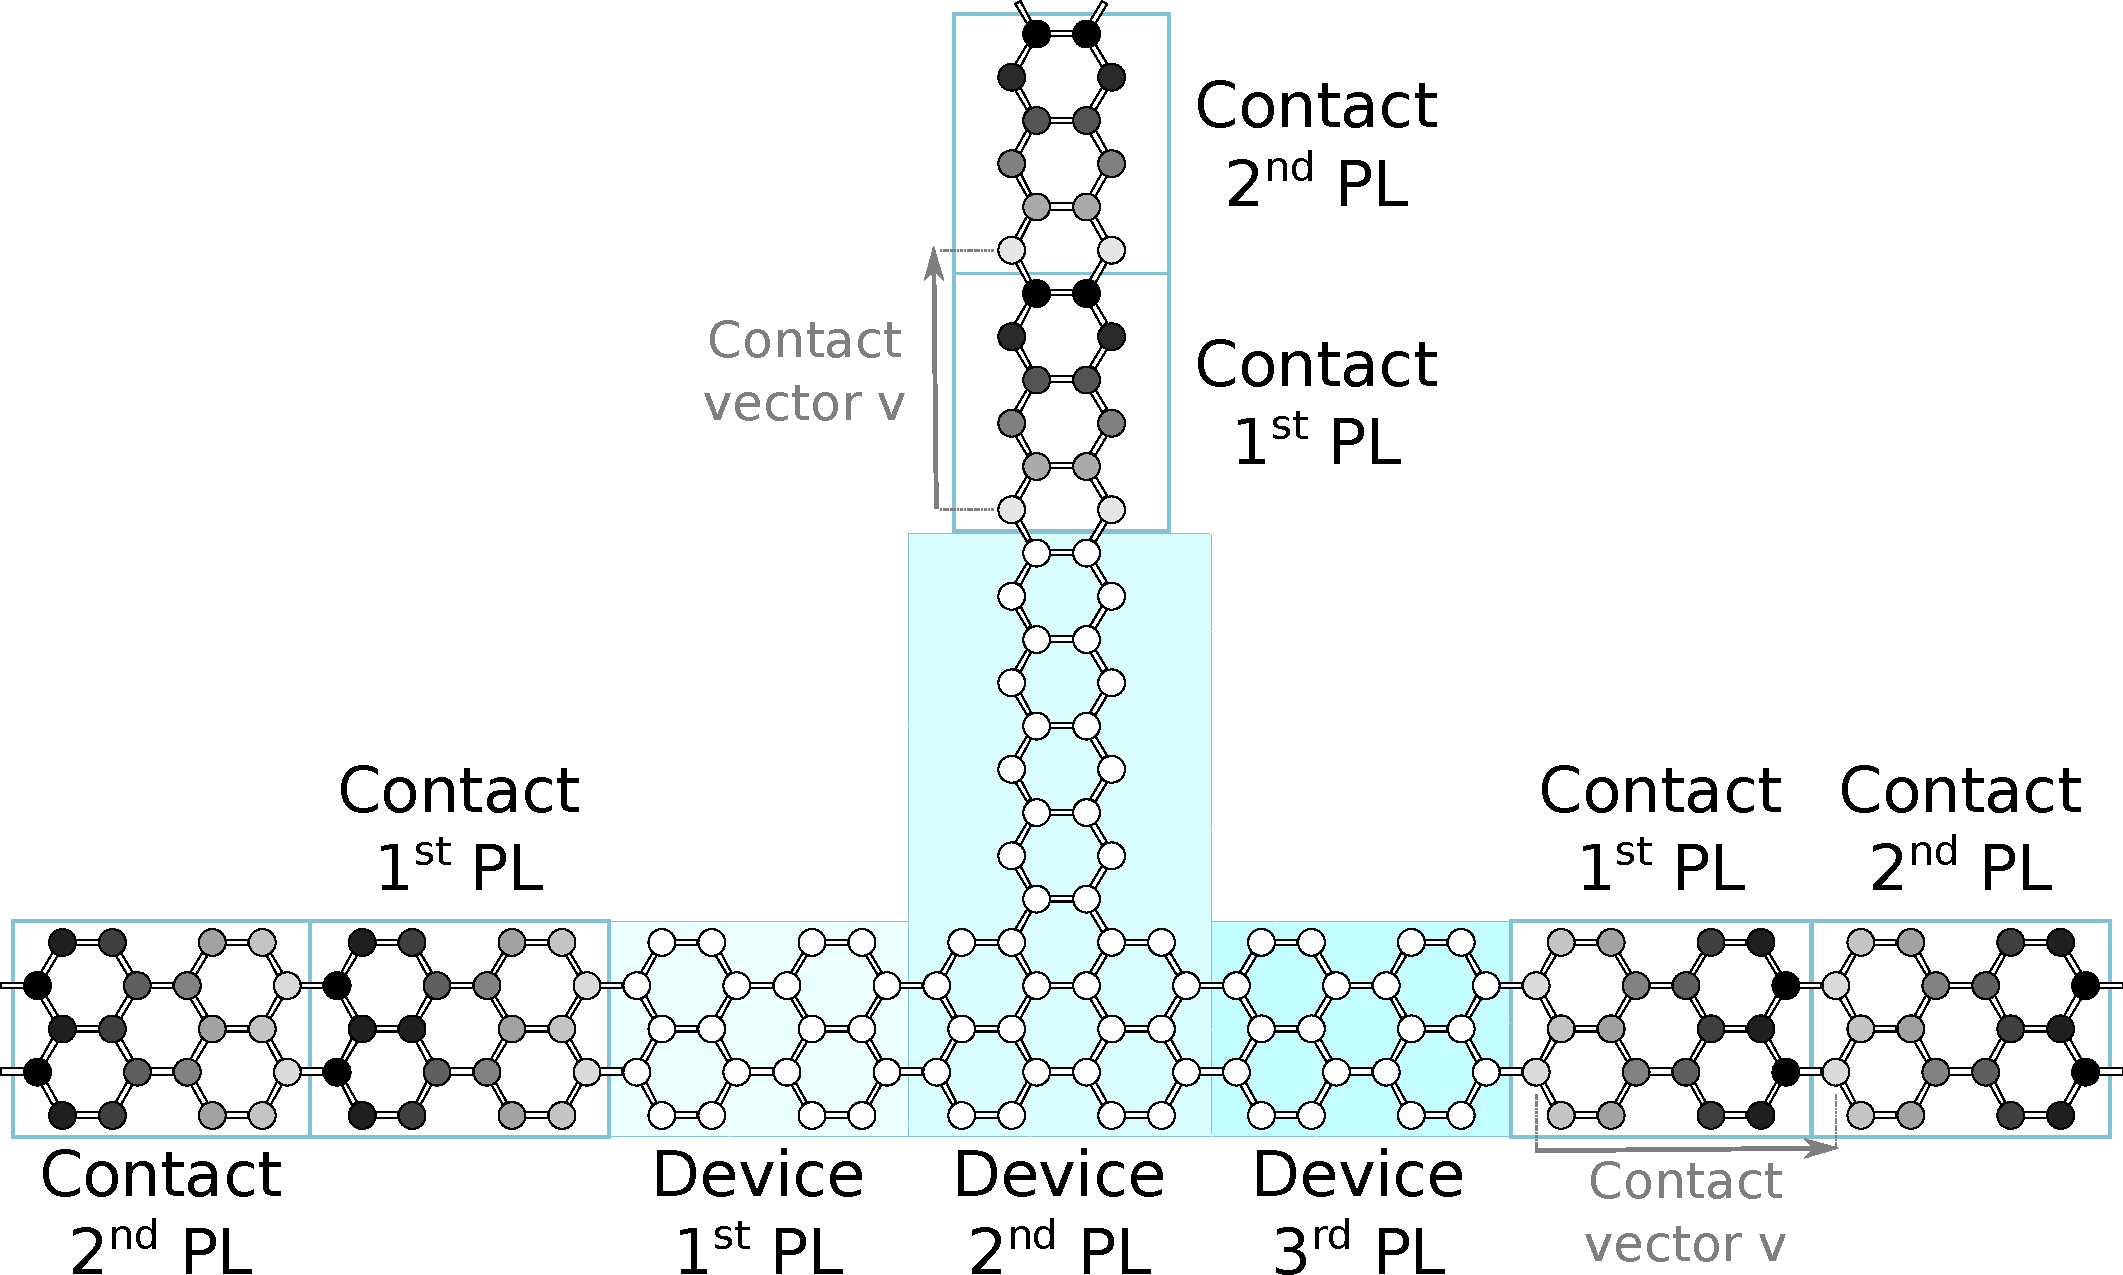
\includegraphics[width=0.8\textwidth]{Fig_device.pdf}
  \end{center}
  \caption{ \label{fig:device} Example of a valid 3 contact device with
    principal layers marked.}
\end{figure}

{\bf Note}:\\ The code {\em does not} currently check: if the device regions are
consistently defined (rules~\ref{rule1} and \ref{rule6}); if the PL defined are
really PLs (rule~\ref{rule3}); or if the first PL defined is really the one
closest to the device (rule~\ref{rule5}).\\ The code {\em does} check rules
\ref{rule4}, \ref{rule8}, \ref{rule9} and \ref{rule10}. The check for
rules~\ref{rule4} and \ref{rule9} is performed on the atomic coordinates, such
that
\begin{equation}
 \mathbf{R}^2_{i+N} = \mathbf{R}^1_i + \mathbf{v}\qquad\forall i \in PL
 \label{eqn:PLcriteria}
\end{equation}
where $\mathbf{R}^2_i$ are atomic coordinates of atoms in the second PL of the
contact, $\mathbf{R}^1_i$ are atomic coordinates of atoms in the first PL and
$\mathbf{v}$ is the contact lattice vector. The equality is verified within an
accuracy that can be set by the user (see below for \is{PLShiftTolerance}).

Please take care when building structures and to cross-check them. Also consider
looking at the examples distributed with the code. The input structure is often
the first suspect when there are problems in transport calculations.


\htcbsection{Transport}
\label{sec:transport.transport}

The Transport section collects together the information needed whenever open
boundary conditions are used. It contains the description of the partitioning of
the system into a {\em device} and the {\em contact} regions and additional
information needed to calculate the required self-energies associated with the
contacts. The transport block contains the following properties:
\begin{ptable}
  \kw{Device} &p& & - & \pref{Device} \\
  \kw{Contact} &p& & - & \pref{Contact} \\
  \kw{Task} & m & & UploadContacts & \pref{Task} \\
  \hline
\end{ptable}

An example transport geometry specification looks like:

\begin{verbatim}
Transport {
    Device {
      AtomRange = 1 8
    }
    Contact {
      Id = "source"
      AtomRange = 9 24
    }
    Contact {
      Id = "drain"
      AtomRange = 25 40
    }
}
\end{verbatim}

Where the associated atomic geometries follow the rules of
Section~\ref{sec:transport.geometry}. In this specific example, there is only
one principal layer in the device, but each contact contains two principle
layers (atoms 9--16 and 17--24 in the ``source'' contact, atoms 25--32 and
33--40 in the ``drain'' contact).

\htcbsubsection{Device} 
The Device blocks contains the following properties:
\label{sec_device}

\begin{ptableh}
  \kw{AtomRange} &2i& & - & \pref{AtomRange} \\
  \kw{FirstLayerAtoms} &i+& & 1 &  \\
  \kw{\new ContactPLs} &i+& \iscb{Geometry = NoGeometry} & 1 1 &  \\
  \hline 
\end{ptableh}

\begin{description}

\item[\is{AtomRange}] \label{AtomRange} defines the first and last atom of the
  device region.

\item[\is{FirstLayerAtoms}] defines the first atom of PLs in the device
  region. By default there is only one layer (the entire device
  region). Alternatively the user can manually reorder and group the atoms in
  the structure into distinct layers for more efficient Green function
  calculations.

  The device layers, unlike the contact PLs, do not need to represent unit cell
  repetitions. If the device geometry has specified principal layers, these must
  be ordered in such a way that all the atoms within each of the layer are
  contiguous in space and adjacent layers must be placed next to each other in
  the structure. This ensures that the constructed hamiltonian and overlap are
  block tri-diagonal. Refer to~\cite{Pecchia_NJP} for a description of the
  efficient iterative Green's function algorithm that can then be applied.
  
{\new  
\item[\is{ContactPLs}] are the indices of PLs coupled to every electrode (e.g. \is{1 7} means the first contact is coupled to the PL number 1, the second contact -- to the PL number 7). Every contact can be coupled to only one of PLs. This property is required for model calculations.  
}


\end{description}

\htcbsubsection{Contact} The contact block contains the following properties:

\begin{ptable}
  \kw{Id} & s &  & &  \\
  \kw{AtomRange} &2i& &  &  \\
  \kw{PLShiftTolerance} & r & & 1E-5 & \\
  \kw{Temperature} & r & & 0.0 & \\
  \kw{FermiLevel} &r& &  &  \\
  \kw{Potential} & r &  & 0.0 & \\
  \kw{WideBand} & l & & No & \\
  \kw{LevelSpacing} & r & WideBand = Yes & 0.735 & \\
  \kw{WriteSelfEnergy} & l & & No & \\
  \kw{ReadSelfEnergy} & l & & No & \\
  \kw{ReadSurfaceGF} & l & & No & \\
  \kw{WriteSurfaceGF} & l & & No & \\
  \kw{Unformatted} & l & & No & \\
  \kw{WriteSeparatedSGF} & l & & No & \\
  \kw{ReadSeparatedSGF} & l & & No & \\
\end{ptable}

The sections \verb|Device| and \verb|Contact| are used to define the atomic
range of each region. The user can also assign a label (\is{Id}) to each contact
that can be used later for cross referencing. In the section \verb|Contact| the
user can add a keyword that specifies the accuracy for the internal check of the
PLs (tolerance for rule~\ref{rule4} of structures, i.e.\ that accuracy to which
\eqref{eqn:PLcriteria} must be satisfied).

\begin{description}
\item[\is{Id}] Assign a text label to the contact (must be 50 or fewer
  characters).
\item[\is{AtomRange}]  Defines the first and last atom of the
  device region.  {\bf Note} the contacts should be defined such that the atoms
  included in the range are in continuous increasing order in the structure.
\item[\is{PLShiftTolerance}]\modif{\modtype{length}} Used to set the absolute
  accuracy used to check principal layer (PL) consistency (see above). The
  default is $10^{-5}$ atomic units. Please be aware that using a large values
  may hide errors due to an inconsistent definition of the contacts, therefore
  it should not be modified.
\item[\is{Temperature}]\modif{\modtype{energy}} Specifies the electronic
  temperature of the contact (see a more detailed discussion after the section 
  \"Analysis\").
\item[\is{FermiLevel}]\modif{\modtype{energy}} Specifies the Fermi level of the
  contact.
\item[\is{Potential}]\modif{\modtype{energy}} Specifies any additional
  electrostatic potential applied to the contact. The natural units of this
  quantity are a potential energy.
\item[\is{WideBand}] Use the wide band approximation for the contact. If set to
  \is{Yes}, the surface Green's function of the contact is not explicitly
  calculated but is instead assumed to be local and constant according to a
  specified density of states.
\item[\is{LevelSpacing}]\modif{\modtype{energy}} Specifies the inverse of the
  density of states (DOS) per atom to be used for the Wide Band
  approximation. As an example, the DOS of gold at the Fermi level is
  0.05~eV$^{-1}$atom$^{-1}$, which corresponds to an energy spacing of 20~eV
  $\approx$0.735~Hartree (the default value).
\item[\is{WriteSelfEnergy}] Write the contact self energy to a single formatted text file
  matching its \is{contactId} and called \verb|contactId-SelfEnergy.mgf|.
\item[\is{ReadSelfEnergy}] Read the contact self energy from a single formatted text file
  matching its \is{contactId} and called \verb|contactId-SelfEnergy.mgf|.
\item[\is{ReadSurfaceGF}] Read the contact retarded Green function from a single
  formatted text file matching its \is{contactId} and called
  \verb|contactId-SurfaceGF.mgf|.
\item[\is{WriteSurfaceGF}] Write the contact retarded Green function to a single
  formatted text file matching its \is{contactId} and called
  \verb|contactId-SurfaceGF.mgf|.
\item[\is{Unformatted}] If set to \is{Yes}, the above mentioned files are written
  in binary instead of text format.
\item[\is{WriteSeparatedSGF}] Write the contact retarded Green functions for every energy separately
  to binary files in the GS directory. 
\item[\is{ReadSeparatedSGF}] Read the contact retarded Green functions for every energy separately
  from binary files in the GS directory. If there are no required files, the SGFs are calculated and
  saved.
\end{description}

\htcbsubsection{Task = ContactHamiltonian} \label{Task} The \is{Task} option is
used to define which type of calculation should be performed. Before performing
a transport calculation it is necessary to compute some equilibrium properties
of the contacts by running a periodic boundary condition DFTB calculation. This
necessary step must be carried out separately for each contact and can be done
by specifying a \kw{Task}=\is{ContactHamiltonian} block, as in the following
example to calculate the source case.

\begin{verbatim}
Task = ContactHamiltonian {
  ContactId = source
  ContactSeparation [Angstrom] = 50.0
}
\end{verbatim}

When \kw{Task}=\is{ContactHamiltonian} the following options can be defined

\begin{ptable}
  \kw{ContactId} & s &  & & \\
  \kw{ContactSeparation} & r & & 1e3 & \\
  \hline
\end{ptable}

\begin{description}
\item[\is{ContactId}] Id label of the contact to be calculated.
\item[\is{ContactSeparation}]\modif{\modtype{length}} Dummy separation in
  transverse direction (see the following explanation).
\end{description}

The contact calculation computes the {\em bulk} Hamiltonian, self-consistent
charges (if SCC) and Fermi level for each contact. This is a usual \dftbp
calculation for which appropriate parameters must be included in the input
file. For {\em supercell} structures the calculation of the contact is performed
using corresponding supercells in which the transverse lattice vectors are those
specified in the \is{Geometry} tag and the lattice vector along the {\em contact
  direction} is deduced from the PL separations (rule~\ref{rule9}). If the
structure is defined as a {\em cluster}, the contact calculation is performed
for a {\em supercell} in which the contact is treated as one-dimensional
periodic wire with a surrounding vacuum region. However, since \dftbp does not
support pure one- and two-dimensional calculations, dummy lattice vectors are
defined for the two remaining directions. The default value for these lattice
vectors is 1000~a.u.\ (527~{\AA}), which should guarantee sufficient wire to
wire distances to avoid Coulomb interactions. The user can specify an
alternative contact separation using the keyword \is{ContactSeparation} placed
in the \kw{ContactHamiltonian} block.  Each contact computation produces one
output file called \verb|shiftcont_ContactId.dat| which storing energy shifts
and Mulliken charges that must be present in the working folder in all
subsequent transport calculations.

{\bf Note} that during the contact calculation you will need to perform a
k-point integration in the contact direction (as the contacts are
semi-infinite).  Whenever the system is defined as a cluster, \dftbp{} will
automatically extract the periodicity vectors from the geometry such that the
first reciprocal vector will correspond to the transport direction.  Therefore you
must specify a k-point sampling for the periodic calculation by sampling along
the first reciprocal lattice vector.  As an example, if the structure is defined
as a cluster (i.e., 1-dimensional wire leads), the source contact calculation
will have an input file similar to:

\begin{verbatim}
...
Task = ContactHamiltonian {
  ContactId = source
}
...
Hamiltonian = DFTB {
...
KpointsAndWeights = SupercellFolding {
     8  0  0   # sampling points here regardless of the transport direction
     0  1  0
     0  0  1
     0.5 0.0 0.0
  }
}
\end{verbatim}

On the other hand, if your structure is defined as a supercell (as an example, a
molecule with bulk contacts) and the transport direction is along the $y$
direction, your the source contact calculation will have an input file similar
to:

\begin{verbatim}
...
Task = ContactHamiltonian {
  ContactId = source
}
...
Hamiltonian = DFTB {
...
KpointsAndWeights = SupercellFolding {
     4  0  0   # points in periodic direction
     0  8  0   # points in transport direction
     0  0  4   # points in periodic direction
     0.5 0.5 0.5
  }
}
\end{verbatim}


This could seem confusing, but the underlining reasons is that in the cluster
calculation the reciprocal lattice is set up by the code itself, while in the
periodic calculation is set up by the user who can chose any arbitrary
direction.  Refer to the transport cookbook and to the distributed examples for
further clarification.

\htcbsubsection{Task = UploadContacts} After the contact calculations, it is
possible to perform actual transport calculations. This is activated simply
specifying \kw{Task = UploadContacts}, without additional options ({\bf Note} if
no task is specified, \dftbp{} assumes \is{UploadContacts} is the required task
in the transport block). In order to set up a proper transport calculation the
user should also define the contacts' Fermi levels (as printed in the files
previously produced by using \is{ContactHamiltonian} tasks) and any required
potential shift for each contact.
\begin{verbatim}
Transport {
  Device {
    AtomRange = 1 8
  }
  Contact {
    Id = "source"
    AtomRange = 9 24
    FermiLevel [eV] = -8.4123
    Potential = 0.0
  }
  Contact {
    Id = "drain"
    AtomRange = 25 40
    FermiLevel [eV] = -8.4123
    Potential = 1.0
  }
  Task = UploadContacts
}
\end{verbatim}

{\bf Note:} During the transport calculation you will not need to set up the
k-point integration when the structure is defined as a cluster, just as in a
regular \dftbp{} calculation. For supercell calculations, integration
perpendicular to the transport direction will need to be accurate, but the
sampling grid can in the transport direction itself can have only a single
value.  In the special case where your device is a supercell but also wire-like,
with a vacuum region lateral to its transport direction, the Gamma-point can be
chosen:
\begin{verbatim}
  KPointsAndWeights = {
    0 0 0  1.0
  }
\end{verbatim}

\htsection{GreensFunction}

For calculations in open systems, instead of calculating the eigenstates of the
system, a Green function method is used to obtain the density matrix of the
system. The Green function (GF) solver can also be used for conventional
supercell/cluster boundary conditions if required.

In order to activate Green function calculations the user must define the
keyword \is{EigenSolver = GreensFunction} in the \is{Hamiltonian} section. The
GF solver, either under equilibrium (no bias applied) or under non-equilibrium
conditions, builds the density-matrix of the device region such that it is
consistent with any contacts that are present. Strictly speaking the GF does not
solve for the eigenstates of the system, however it logically substitutes the
traditional construction of the density matrix from the eigenstates of the
system, as would be obtained after the diagonalisation step. The usual \dftbp{}
self-consistent calculations can be driven using the GF solver.

The following table gives the important parameters of the solver:
\begin{ptableh}
  \kw{Verbosity} & i & & Options\%Verbosity & \\
  \kw{Delta} & r  &  & 1E-5 & \\
  \kw{ContourPoints} & 2i &  & 20 20 &  \\
  \kw{LowestEnergy}  & r  &  & -2.0 & \\
  \kw{FermiCutoff}  & i & & 10 & \\
  \kw{EnclosedPoles} & i & & 3 & \\
  \kw{RealAxisStep} & r & RealAxisPoints=undefined & 6.65E-4 & \\
  \kw{RealAxisPoints} & r & RealAxisStep=undefined &  & \\
  \kw{SaveSurfaceGFs} & l & & Yes & \\
  \kw{ReadSurfaceGFs} & l & & No & \\
  \kw{FirstLayerAtoms} & i+ & Transport = undefined & 1 & \\
  \kw{FermiLevel} & r& Transport = undefined &  & \\
  \kw{LocalCurrents} & l&  & No & \\
\end{ptableh}

Note: For efficient GF calculation the device region must be partitioned into
layers whose fundamental property is to interact with nearest-neighbour layers
only (see section~\ref{sec:transport.geometry}).

\begin{description}
  \item[\is{Verbosity}] This parameter controls the level and amount of output
  messages and takes values ranging from 1 to 100. The default value is equal to
  the \is{Verbosity} parameter of \is{Options} block. 
\item[\is{Delta}]\modif{\modtype{energy}} A small positive imaginary delta used
  in the GF definition and required for the x contour integration.
\item[\is{ContourPoints}] The number of points along the complex contour
  integration of the GF along the segments $\mathcal{C}$ and $\mathcal{L}$ (see
  contour integration in section~\ref{sec:transport.contourint}).
\item[\is{LowestEnergy}]\modif{\modtype{energy}} The initial energy from which
  the integration starts. It should be low enough to ensure that all the
  electronic states are correctly included in the integration. The default is
  -2.0 Hartree (see contour integration).
\item[\is{FermiCutoff}] Integer number setting the Fermi distribution cutoff in
  units of $kT$. It is read only if the Fermi distribution temperature is
  greater than 0 (see contour integration).
\item[\is{EnclosedPoles}] The number of Poles enclosed in the contour. It is
  meaningful only in finite temperature calculations (see contour integration).
\item[\is{RealAxisStep}]\modif{\modtype{energy}} The energy step along the real
  axis integration for non-equilibrium calculations. Note: \kw{RealAxisStep} and
  \kw{RealAxisPoints} cannot both be defined at the same time.

\item[\is{RealAxisPoints}] The number of points along the real axis integration
  needed in non-equilibrium calculations. The default depends on the electronic
  temperature and bias. Note: \kw{RealAxisStep} and \kw{RealAxisPoints} cannot
  both be defined at the same time.

\item[\is{SaveSurfaceGFs}] As the SCC cycle usually needs to repeat the
  calculation of the Green's function at given energy points and as the surface
  Green functions do not change during the SCC cycle, this flag allows for
  saving the surface Green functions to disk and so save computational time on
  every SCC cycle after the first.

\item[\is{ReadSurfaceGFs}] Loads the surface Green's function from a file at the
  the first SCC cycle. Note that this operation only makes sense if the energy
  integration points are identical to the calculation used to generate the
  surface Green's function files. The code does not verify whether this
  condition is fulfilled. In general there is no need to modify the defaults for
  \kw{ReadSurfaceGFs} and \kw{SaveSurfaceGFs}.

\item[\is{FirstLayerAtoms}] As described in Device block. Can be specified only
  if no \kw{Transport} block exists.  {\bf Note:} the Green solver can be used
  also to calculate the density matrix when there are no open boundary
  conditions, for example to take advantage of the iterative scheme in quasi-1d
  systems. In this case, a \kw{Transport} block is not defined and therefore
  \iscb{FirstlayerAtoms} should be given in the \is{GreensFunction} block. Also,
  the Fermi level of the system must be known and provided to fill up the
  electronic states.

\item[\is{FermiLevel}]\modif{\modtype{energy}} Required to set the Fermi level
  used by the Green solver to fill up the electronic states, unless already
  specified by there being contacts already present.

\item[\is{LocalCurrents}] If set to \is{Yes}, local bond-currents are computed using
  the non-equilibrium density matrix.  This task is currently limited to
  \textbf{non-periodic} systems. The output is placed in a file
  \verb|lcurrent_u.dat| (or \verb|lcurrent_d.dat| depending on spin).  The files
  are arranged in a table in order of increasing neighbour distance,

\begin{tabular}{|c|c|c|c|c|c|c|c|c|c|c|c|}
  \hline
  Atom(i) & x & y & z &  nNeighbours &  j1 & I$_{i,j1}$ & j2 & I$_{i,j2}$ &  j3 & I$_{i,j3}$ & ...\\
  \hline
\end{tabular}

  This file can be processed using the small code \verb|flux| provided in
  tools/transport that helps in building plots for jmol.
\end{description}

GreensFunction section example:

\begin{verbatim}
Eigensolver = GreensFunction {
  FirstLayerAtoms = 1 61 92 145
  Delta [eV] = 1E-4
  ContourPoints = 20 20
  RealAxisPoints = 55
  LowestEnergy [eV] = -60.0
  FermiCutoff = 10
  EnclosedPoles = 3
}
\end{verbatim}


\section{Eigensolver = TransportOnly}

The \is{GreensFunction} block is used to solve the full self-consistent NEGF
transport problem. However, the block \iscb{TransmissionAndDos} within the
\is{Analysis} block (see below), can be used to calculate the transmission
function according to the Landauer formula, without solving for the full density
matrix. This can be applied even for calculations where the density matrix and
charge densities are not computed. Similarly, in these cases the electrostatics
block should be omitted (i.e.\ the \is{Electrostatics = Poisson}). The keyword
\is{Eigensolver = TransportOnly} is used to jump straight to the post-SCC
analysis.  \textbf{Note:} This option cannot be used together with calculations
which require forces, including geometry relaxations or md calculations.


\section{Contour integration}
\label{sec:transport.contourint}

Much of the computational work for transport is in the integration of the energy
resolved density matrix, as represented via the NEGF matrix. The integration is
efficiently performed with a complex contour integration and a real axis
integration, as shown in Figure~\ref{fig:contour} and discussed in
references~\cite{Pecchia_spring, Pecchia_RPP, Pecchia_NJP}.
\begin{figure}[!h]
  \begin{center}
    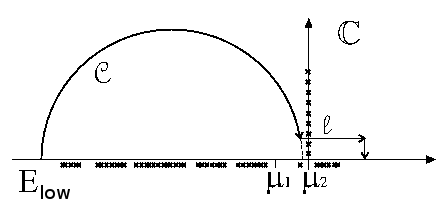
\includegraphics[width=8.0cm]{Fig_integration.png}
    \caption{ \label{fig:contour} Contour integration in the complex plane for
      the Green's functions. The crosses represent poles of either $G^r$ or the
      Fermi function.}
  \end{center}
\end{figure}
All integrations are performed with Gaussian quadratures and the number of
points must be specified manually. The complex contour integration is subdivided
into two sections: the first section is the arc of a circle, $\mathcal{C}$, that
can be computed with a few integration points (default 20); the second section
is a line that intersects the contour and runs parallel to the real axis at a
distance that depends on the number of poles of the Fermi function that are
enclosed within the contour. Usually a good choice for the number of poles is
between 3 and 5 (the default is 3). The poles are placed at the complex points
$z_m = E_F + i (2m+1) \pi k_B T$ and therefore are separated from each other by
$2 \pi k_B T$, where $k_B$ is Boltzmann's constant.  At $T=300$~K this
corresponds to a separation of 156~meV. It should be noted that, as the
temperature decreases, the separation between poles reduces. This makes the
contour integration harder as it needs to walk across two singularities. At very
low temperatures, $T=10$~K, the separation is 5.2~meV. Below this temperature,
the contour integration is treated as $T=0$ in order to avoid numerical
inaccuracies. The integration along the segment $\mathcal{L}$ extends up to
$Re\left[ z \right] = E_F + n k_B T$, where $n$ is an integer number specified
by the keyword \kw{FermiCutoff} and has a default value of 10.  In the limit
$T=0$~K the poles collapse into a non-analytic branch cut and the contour needs
to be changed such that the second section of the complex contour becomes the
arc of circle closing on the real axis.  Finally, the real axis integration
extends between the lowest and highest chemical potentials. The number of
quadrature points should depend on the bias itself and can be set using
\kw{RealAxisPoints} or \kw{RealAxisStep}. The default value is $1\text{~pt} /
0.018\text{~eV}$ (actually $1500\text{~pt} / 1\text{~Hartree}$). In finite
temperature calculations the segment is extended to include the Fermi cutoff by
$n k_B T$ on both sides ($\mu_1 - n k_B T, \mu_2 + n k_B T$). In this case the
number of quadrature points are increased by assuming the same point density
defined in the range ($\mu_1, \mu_2$).  Example: for a bias of 0.2~V, the
default number of points is $0.2 \cdot 1500 / 27.21139 = 11$. At $T=300$~K the
interval is increased by 0.26~eV on both sides, therefore $0.26 \cdot 1500 /
27.21139 = 14.33$ which is truncated to 14 points, leading to a total of 38
points along the real axis. The use of the keyword \kw{RealAxisStep} is usually
more convenient because it ensures a consistent real axis integrations during,
for example, a bias sweep.

Note: The GF solver can be used also for calculations other than the transport
context. In cases where the position of the Fermi Energy is known with good
accuracy, the density matrix solver based on the GF can be used to compute the
electronic properties of clusters and supercells. The recursive algorithm may be
an efficient solution to large problems having an elongated one dimensional
shape.

\section{Spin-polarised transport}

Spin-polarised transport is not available yet. Collinear spin transport will be
available soon, as all the needed machinery has been implemented and is
undergoing debugging and testing.


\section{Poisson solver}

The Poisson solver is a fundamental part of charge self-consistent
non-equilibrium transport calculations and must be declared whenever an SCC NEGF
calculation is performed using \is{Electrostatics = Poisson}. Under
non-equilibrium conditions the self-consistent potential of the KS equations
cannot be solved using the efficient $\gamma$-functional, but instead requires
the definition of appropriate boundary conditions for the potentials imposed by
the contacts. However, since the $\gamma$-functional is functionally related to
a pure Hartree potential, it can be obtained in real space by solving a Poisson
solver.  The Poisson equation is solved in a {\em box} with hexahedral prism
shape. This restriction is imposed by the Poisson solver being employed. This
restricts calculations of supercell structures to orthorhombic super-lattices.
An additional restriction is that the box sides must be aligned with the
Cartesian axes, $x$, $y$, $z$.

\begin{ptableh}
  \kw{Verbosity} & i & & Options\%Verbosity & \\
  \kw{PoissonBox} & 3r & &  &  \\
  \kw{BoxExtension} & r &  & 0.0 &  \\
  \kw{MinimalGrid} & 3r  &  & 0.3 0.3 0.3 & \\
  \kw{PoissonAccuracy} & r &  & 1E-7 &  \\
  \kw{AtomDensityTolerance}  & r  &  & 1E-6 & \\
  \kw{AtomDensityCutoff}  & r  &  & 14.0 & \\
  \kw{CutoffCheck} & l & & Yes & \\
  \kw{NumericalNorm}  & l  &  & No & \\
  \kw{SavePotential} & l & & No & \\
  \kw{PoissonAccuracy} & r & & 1E-6 & \\
  \kw{MaxPoissonIterations} & i & & 60 & \\
  \kw{BuildBulkPotential} & l & & Yes & \pref{Boundary Conditions}\\
  \kw{ReadOldBulkPotential} & l & & Yes & \pref{Boundary Conditions} \\
  \kw{OverrideDefaultBC} & m & & none\{\} & \pref{Boundary Conditions}\\
  \kw{OverrideBulkBC} & m & & none\{\} & \pref{Boundary Conditions}\\
  \kw{BoundaryRegion} & m & & global\{\} &  \pref{Boundary Conditions} \\
  \kw{Gate} & m & & none\{\} & \pref{Electrostatic Gates} \\
  \kw{MaxParallelNodes} & m & & none\{\} & \pref{Parallelisations} \\
  \kw{RecomputeAfterDensity} & l & & No & \\
\end{ptableh}


\begin{description}
  
\item[\is{Verbosity}] This parameter controls the level and amount of output
  messages and takes values ranging from 1 to 100. The default value is equal to
  the \is{Verbosity} parameter of \is{Options} block. 
\item[\is{PoissonBox}]\modif{\modtype{length}} Dimension of the Poisson box
  along the directions $x$, $y$ and $z$. 
\item[\is{BoxExtension}]\modif{\modtype{length}} With this value it is possible
  to tune the position of the box interface between the device and contacts.  By
  default (\is{BoxExtension}=0.0) the boundary is placed at the midpoint between
  the last device atom and the first contact atom.
\item[\is{MinimalGrid}]\modif{\modtype{length}} The minimal requested grid
  spacing along $x$, $y$ and $z$. The actual grid spacing chosen by the
  multigrid solver will be lower than this.
\item[\is{AtomDensityTolerance}] In order to calculate the potential, the
  Mulliken charges are projected on the real space grid. This parameter defines
  the cutoff after which the charge is considered to vanish (i.e., the spatial
  extension of the projected charge). The default is 1E-6~e. Note that the
  contacts must be at least twice the length over which a projected Mulliken
  charge extends. If this conditions is not fulfilled and \is{CutoffCheck} is
  set to \is{Yes}, the code will exit with an error message. Setting this
  parameter to a lower value could allow shorter contacts to be defined in some
  cases. However this could lead to error in the potential and hence to spurious
  reflections, therefore it should be left at its default value (or changed very
  carefully).
\item[\is{AtomDensityCutoff}]\modif{\modtype{length}} Defines the atomic radius
  cutoff. This is an alternative to \is{AtomDensityTolerance} and directly
  specifies the distance over which charge density associated with an atom is
  considered to vanish.
\item[\is{CutoffCheck}] If set to \is{No}, consistency between contact length
  and charge extension is not verified (see \is{AtomDensityTolerance} and/or
  \is{AtomDensityCutoff}). The default is \is{Yes}. As with
  \is{AtomDensityTolerance}, this parameter should not be changed unless you
  know exactly what you're doing.
\item[\is{SavePotential}] Save the electrostatic potential to the file
  \verb|potential.dat| and the charge density to \verb|charge_density.dat|.
  Additional files \verb|Xvector.dat|, \verb|Yvector.dat|, \verb|Zvector.dat|
  and \verb|box.dat| are also created. These files can be converted to a cube
  file that can be visualised in jmol. See section~\ref{sec:transport.tools}
  about transport tools.
\item[\is{PoissonAccuracy}] Defines the accuracy for the approximate solution of
  the Poisson equation (default value 10$^{-6}$).
\item[\is{MaxPoissonIterations}] Defines the maximum number of iterations allowed
  for the solver.
\item[\is{RecomputeAfterDensity}] When set to \is{Yes}, Poisson's equation is
  solved again after the density matrix is created in order to make the
  electrostatic energy consistent with the newly updated charges.  In transport
  calculations it is set to \is{No} by default in order to avoid the extra time
  spent on the Poisson step. This does not affect the SCC loop or other
  calculations apart from the electronic energy and forces.
\end{description}

{\bf Note}: The Poisson box can be specified using the keyword
\verb|PoissonBox|. In calculations where two contacts face each other along the
same axis, setting the box-size along this axis will has no effect (the code
adjusts to the correct size internally). The \is{PoissonBox} keyword is
redundant (and should not be specified) when the system is periodic, since in
this case the box geometry is taken from the supercell lattice vectors.

Numerical error in the potential will results in spurious discontinuities at the
contact-device interfaces. The default tolerances should be sufficient to avoid
this in most cases.

Below is a a typical example of the whole Poisson block specification. Some of
the keywords are described in the next subsections.
\begin{verbatim}
 Electrostatics = Poisson {
  PoissonBox [Angstrom] = 20.0 20.0 20.0
  MinimalGrid [Angstrom] = 0.3 0.3 0.3
  SavePotential = No
  BuildBulkPotential = Yes
  ReadOldBulkPotential = No
  BoundaryRegion = Global {}
  PoissonAccuracy = 1E-7
  Gate = Planar{
      GateLength_l [Angstrom] = 10.0
      GateLength_t [Angstrom] = 20.0
      GateDistance [Angstrom] = 7.0
      GatePotential [eV] = 1.0
  }
}
\end{verbatim}

\htsubsection{Boundary Conditions}

The Poisson equation is solved imposing boundary conditions (BC) on the
potential at the six faces of the Poisson Box. In transport calculations for
non-supercell geometries comprising two contacts placed along the same axis, the
BCs are chosen as follows:
\begin{itemize}
\item[Dirichlet] fixed potentials on the two contact faces with values defined
  by the applied potentials (see \is{UploadContacts}).
\item[Neumann] zero normal field on the remaining 4 lateral box faces
\end{itemize}
In periodic supercells the BCs are: {\bf Dirichlet} (fixed potentials) on the
two contact faces with values defined by the applied potentials (see
\is{UploadContacts}) and {\bf Periodic} on the remaining 4 lateral box faces.

In some specific cases Neumann BCs can be set on one contact. In order to do so
it is necessary to use \is{OverrideDefaultBC} (see below).

The device and contact potentials should smoothly join at the interface. In
order to achieve this the code computes the bulk potential of each contact and
uses the result as a BC on the contact face of the Poisson box. This is useful
when the contact potential is not uniform due to charge rearrangements. Any
externally applied contact potential (\kw{Potential}) is added to the bulk
potential.  The user can deactivate this calculation by setting the keyword
\kw{BuildBulkPotential} to \is{No}.

{\bf Note}: The bulk potential is computed on a special box that has ``lateral''
sizes copied from the device box, and has the size of one PL along the contact
direction. The BCs are---so to speak---inherited from the device region. In
particular:
\begin{enumerate}
\item Along the contact direction periodic BCs are imposed on both faces.
\item On the other four faces the BCs are copied from the device region
  (supercell or cluster).
\item The user can override this setting using \verb|OverrideBulkBC| (see
  below).
\item When all four faces inherit Neumann BC (default for the device region),
  these are {\em ALL} internally changed to Dirichlet, because the solver cannot
  handle this situation as it gives rise to a singular matrix.
\end{enumerate}

\begin{description}
\item[\is{BuildBulkPotential}] (default: \is{Yes}) is used to calculate the
  electrostatic potential of the contacts and the result is used as a Dirichlet
  boundary condition on the contact face (superimposed to the contact
  potential).
\item[\is{ReadOldBulkPotential}] Read a previously computed bulk potential from
  hard-disk.
\item[\is{BoundaryRegion}] Specifies how the Dirichlet boundary conditions are
  treated on each contact face of the Poisson box. It can be \kw{Global},
  \kw{Square} or \kw{Circle}. \kw{Global} means that the BC is applied to the
  entire face of the box, whereas the other keywords imply that the Dirichlet BC
  are applied on a cross-section projected on the contact face. This is useful
  for instance when handling nanowire contacts, for which it is not really
  correct to impose a constant potential on the whole face of the Poisson box.
\item[\is{BufferLength}]\modif{\modtype{length}} can be used to set the size of
  the boundary region beyond the atomistic size which is determined as the
  minimal circle or square containing all atoms of the contact cross-section.
\end{description}

\begin{ptableh}
  \kw{BufferLength} & r &  & 9.0 &  \\
\end{ptableh}

Example:
\begin{verbatim}
BoundaryRegion = Circle {
    BufferLength [Angstrom] = 3.0
}
\end{verbatim}

In some special cases it might be necessary to override the default BCs applied
by the code to the Poisson equation. Currently this can be done using the
keywords: \verb|OverrideDefaultBC| and \verb|OverrideBulkBC|.

\begin{description}
\item[\is{OverrideDefaultBC}] block is used to override the BCs described
  above. It can be used to force Dirichlet or Neumann BCs along some specified
  directions or on one of the four lateral faces of the Poisson box.
\item[\is{Boundaries}] is used to specify on which face different BCs must be
  imposed. Assuming contacts are aligned along $z$, the keyword can be set to be
  any of \is{xmin}, \is{xmax}, \is{x}, \is{ymin}, \is{ymax} or \is{y}.
\end{description}

\begin{verbatim}
OverrideDefaultBC = Dirichlet {
      Boundaries = xmin
}
\end{verbatim}

For instance, setting a Dirichlet BC on \verb|Boundaries = xmin| imposes
$\phi(x,y,z)=0$ on the face placed at $x=x_{\text{min}}$, while
\verb|boundaries = xmax| would impose $\phi(x,y,z)=0$ on the face placed at
$x=x_{\text{max}}$. When Dirichlet needs to be forced on both faces it is
possible to use either \verb|boundaries = xmin,xmax| or simply
\verb|boundaries = x|. The same syntax can be used to impose conditions on more
faces, using \verb|boundaries = x,y| or \verb|boundaries = x,ymin|.

A similar strategy can be used to impose different boundary conditions on the
contacts. For instance, a Neumann BC can be set on one contact face by using

\begin{verbatim}
OverrideDefaultBC = Neumann {
      Boundaries = zmin
}
\end{verbatim}

{\bf Note} that the user should know which face of the Poisson Box corresponds
to the desired contact. Furthermore, if the user sets Neumann at all contacts
the Poisson solver will not converge (singular matrix) unless the Dirichlet
condition is imposed somewhere else (e.g., a gate potential is present).

It is also possible to override the default BCs when computing the bulk
potential.

\begin{description}
\item[\is{OverrideBulkBC}] block is used to override bulk BC usually copied from
  the device region.
\item[\is{Boundaries}] has the same meaning and syntax as in
  \verb|OverrideDefaultBC|.
\end{description}

For example by choosing
\begin{verbatim}
OverrideBulkBC = Neumann {
      Boundaries = x, y
}
\end{verbatim}



\htsubsection{Electrostatic Gates}

The option \kw{Gate} can be used to specify an electrostatic gate. Currently the
available gate types are \kw{Planar} and \kw{Cylindrical}.  There are some
restrictions as the planar gate must be placed with its face parallel to the x-z
plane, i.e., the gate direction must be along y. At the same time the transport
direction should be along the z-axis (i.e.\ perpendicular to the gate). The
latter is not really a restriction but it gives meaning to ``longitudinal'' (l)
and ``transverse'' (t) in the geometrical definitions of the gate
lengths. Example:
\begin{verbatim}
Gate = Planar {
    GateLength_l [Angstrom] = 20.0
    GateLength_t [Angstrom] = 20.0
    GateDistance [Angstrom] = 7.0
    GatePotential [eV] = 1.0
}

Gate = Cylindrical {
    GateLength [Angstrom] = 10.0
    GateRadius [Angstrom] = 7.0
    GatePotential [eV] = 1.0
}
\end{verbatim}

The various options for the gates have the following meanings:
\begin{description}
\item[\is{GateLength\_l}]\modif{\modtype{length}} Sets the gate length along the
  transport direction (always assumed to be $z$). The gate is centred in the
  middle of the device region.
\item[\is{GateLength\_t}]\modif{\modtype{length}} Sets the gate extent
  transverse to the transport direction (assumed to be $x$). The gate is centred
  in the middle of the device region.
\item[\is{GateDistance}]\modif{\modtype{length}} Sets the distance of the gate
  from the centre axis of the device region.
\item[\is{GatePotential}]\modif{\modtype{energy}} Sets the potential applied to
  the gate.
\item[\is{GateRadius}]\modif{\modtype{length}} For a cylindrical gate, sets the
  distance of the gate from the centre axis or gate radius.
\end{description}

\begin{ptableh}
  \kw{GateLenth\_l} & r &  & 0.0 &  \\
  \kw{GateLenth\_t} & r &  & 0.0 &  \\
  \kw{GateDistance} & r &  & 0.0 &  \\
  \kw{GatePotential} & r &  & 0.0 &  \\
  \kw{GateRadius} & r &  & 0.0 &  \\
\end{ptableh}

Note that the gate option has not be tested thoroughly and may still contain
bugs.  Please report any problems you encounter to the developers.

%Developments. In forthcoming releases also double gates will be possible.

%Similarly to a usual \dftbp{} calculation, the output from a Transport calculation
%will be present in the \verb|detailed.out| and \verb|detailed.xml|. These
%files are self-documenting, i.e. you will find a human-readable description of
%the output data in the files themselves. After a transport calculation, the
%files will contain the transmission coefficient for every energy point and for
%every k point and the local density of states for every energy point and
%projection ranges specified in input. They will also contain the total current
%and the partial current for every k point. In a multi-terminal calculation, this
%data will be written for every terminal couple.

\section{Model Hamiltonians} 
\label{sec_model}

To use the external Hamiltonian without geometry \big(if \is{Geometry = NoGeometry\{\}}\big), the type of the Hamiltonian must be set to \iscb{Model}:
\invparskip
\begin{verbatim}
  Hamiltonian = Model{}
\end{verbatim}

The \iscb{Model} method must contain the \is{NumStates} parameter and optional \iscb{HamiltonianMatrix} and \iscb{OverlapMatrix}. If \iscb{HamiltonianMatrix} is not given, default file H.mtr with the Hamiltonian matrix should present.  

All properties of the \iscb{Model} method are:
\begin{ptableh}
  \kw{NumStates} & i &  & -  & \\
  \kw{HamiltonianMatrix} & N$^2$r\footnotetext{N=NumStates} & & $<<<$ H.mtr & \\
  \kw{OverlapMatrix} & N$^2$r & & Unity matrix & \\
  \kw{Dephasing} & p & & &  \pref{sec_deph} \\
  \kw{SpinDegeneracy} & l & & No & \\
  \kw{Orthonormal} & l & & No & \\
  \kw{OrthonormalDevice} & l & & No & \\
  \hline
\end{ptableh}

\begin{description}

\item[\is{NumStates}] is a full number of states in the Hamiltonian including the electrodes. Required for model calculations without geometry. 

\item[\is{HamiltonianMatrix}]\modif{\modtype{energy}} is an array of real numbers.
  
\item[\is{OverlapMatrix}] is an array of real numbers. This property is not required, the default is unity matrix (orthogonal basis).

\item[\is{Dephasing}] Two models of elastic dephasing ("B\"uttiker probe" and "vibronic dephasing") can be used now to include the dephasing and dissipation beyond the coherent Green function method. Thus, we made a new step towards realistic material and device modeling. See Sec.\,\ref{sec_deph}.

\item[\is{SpinDegeneracy}] When set to \is{Yes}, the same Hamiltonian is assumed for spin-up and spin-down.   

\item[\is{Orthonormal}] When set to \is{Yes}, L\"{o}wdin orthogonalization is performed to full Hamiltonian.

\item[\is{OrthonormalDevice}] When set to \is{Yes}, L\"{o}wdin orthogonalization is performed only to the central ``device'' part.
  
\end{description}

{\bf Note}: The structure of the Hamiltonian must be consistent with the definition of transport geometry in  Sec.\,\ref{sec:transport.transport} and follow the same rules as discussed in Sec.\,\ref{sec:transport.geometry}: first the central region, then electrodes one by one, every from two blocks. For two electrodes it looks like
%
\begin{equation}
{\matr H}=\left(\begin{array}{ccccc}
{\matr H}_C & {\matr V}_{CL} & 0 & {{\matr V}_{CR}} & 0 \\
{\matr V}^\dag_{CL} & {{\matr H}_{L0}} & {{\matr H}_{L1}} & {0} & 0 \\
0 & {{\matr H}^\dag_{L1}} & {{\matr H}_{L0}} & 0 & 0 \\
{{\matr V}^\dag_{CR}} & {0} & 0 & {{\matr H}_{R0}} & {\matr H}_{R1} \\
0 & 0 & 0 & {\matr H}^{\dag}_{R1} & {\matr H}_{R0} 
\end{array}\right)
\end{equation}

Example\footnote{The input/output for this and other examples one can find in /external/examples/Model/.}:  
\invparskip    
\begin{verbatim}
  Hamiltonian = Model {
    NumStates = 5 
    HamiltonianMatrix [eV] = {
      1.00    0.10    0.00    0.20    0.00    
      0.10    0.00    1.00    0.00    0.00    
      0.00    1.00    0.00    0.00    0.00    
      0.20    0.00    0.00    0.00    1.00    
      0.00    0.00    0.00    1.00    0.00   
    }
  }
\end{verbatim}
%
In this example a single level with the energy 1 eV is coupled to the left electrode with the coupling $V_{CL}=0.1$ eV and to the right electrode $V_{CR}=0.2$ eV.
    
Instead, the name of the data file can be included in the standard way:
\invparskip
\begin{verbatim}
  HamiltonianMatrix [eV] = { <<< "filename" }
\end{verbatim} 

Model Hamiltonians are used at the moment only for transport calculations. It is important to add the property \iscb{ContactPLs} to the \iscb{Device} section (see Sec.\,\ref{sec_device}). 

\section{Quasi-elastic dephasing}
\label{sec_deph}

To switch on the dephasing effects, the group \iscb{Dephasing} must be included into the Hamiltonian group.
The \iscb{Dephasing} group may contain the following methods/properties:

\begin{ptableh}
  \kw{BuettikerProbes} & m &  & none\{\}  & \pref{BuettikerProbes} \\
  \kw{VibronicElastic} & m &  & none\{\}  & \pref{VibronicElastic} \\
  
  \hline
\end{ptableh}

\htcbsubsection{BuettikerProbes}

\begin{description}
  
\item[\is{BuettikerProbes}] switches on the B\"uttiker probe dephasing. There are two methods: \iscb{ZeroPotential} and \iscb{ZeroCurrent}. The first one describes physical conducting environment with fixed (at the moment zero) electrical potential. The second is for the {\it B\"uttiker Probe Model} of dephasing, when the zero-current condition is fulfilled by artificial adjustment of local electrical potentials.
  
Examples\footnote{The examples of input/output one can find in /external/examples/Dephasing/.}:  
\invparskip    
\begin{verbatim}   
  BuettikerProbes = ZeroPotential {
    Coupling [eV] = constant { 0.01 }
  }

  BuettikerProbes = ZeroCurrent {
    Coupling [eV] = constant { 0.01 }
  }
\end{verbatim}

\end{description}  

\begin{description}
\item[\is{Coupling}]\modif{\modtype{energy}} describes coupling to the environment. The method \iscb{constant} couples all states equivalently. The other possible methods are \iscb{AtomCoupling} -- with different couplings for different atoms, and \iscb{AllOrbitals} -- with different couplings for all atomic orbitals. For the model calculations these two options are equivalent. 
\invparskip
\begin{verbatim}   
  Coupling [eV] = AtomCoupling {
    AtomList { Atoms = 1
               Value = 0.1
    }
    AtomList { Atoms = 2 3
               Value = 0.01
    }
    AtomList { Atoms = 4 5
               Value = 0.03
    }
  }

  Coupling [eV] = AllOrbitals { 0.1 0.1 0.1 ... }
\end{verbatim}

\end{description}  
  
\htcbsubsection{VibronicElastic}

\begin{description}

\item[\is{VibronicElastic}] switches on the quasi-elastic vibronic dephasing method. There is only one method \iscb{local} available at the moment. The \iscb{Coupling} method can get the same values as for B\"uttiker probe dephasing. There are several additional options: 
  \is{AtomBlock} (default=.false.), which changes the way of coupling between electrons and phonons; \is{MaxNumIter} -- the maximum number of iterations (default=100); \is{Mixing} -- control of mixing in the self-consistent cycle (default = 0.05); \is{Tolerance} -- control of the convergency tolerance (default = 0.001).

Example:  
\invparskip  
\begin{verbatim}
  VibronicElastic = local {
    AtomBlock = Yes
    Coupling [eV] = Constant {0.01}
    MaxNumIter = 1000
    Mixing = 0.5
    Tolerance = 0.001
  }
\end{verbatim}
  
\end{description}

\section{Application to STM spectroscopy}
\label{sec_stm}

\htsection{Parallelisations}

The code has been parallelised in two main parts. The Non-equilibrium Green's
functions are computed by distributing the energy points along the contour and
real axis calculations. Contour and real axis integrations are independent and
separately distributed. Load balancing has to be taken care of by the user. For
instance if ContourPoints = \{20 20\} (i.e. 40 in total) and RealAxisPoints =
60, by setting 10 MPI nodes, each node will handle 4 points along the contour
and 6 points along the real axis.

Mixed OpenMP/MPI calculations are possible. When compiling \dftbp{} the user
should link against threaded BLAS/MKL, rather than sequential. Numerical
experiments show that best performance on multicore CPUs is generally obtained
by running independent MPI processes on physical sockets and exploiting OpenMP
multithreading within each socket. For instance NEGF can exploit threaded
matrix-matrix products. The user can experiment by setting the environment
variable\\ {\tt OMP\_NUM\_THREADS}.

The Poisson solver itself has not been parallelised yet. Currently the assembly
of the charge density on the real-space grid and the projection of the potential
onto the atoms has been parallelised. Since the gathering of the charge density
on each node can easily hit communication bottlenecks, the user can use the
parameter \kw{MaxParallelNodes} to control distributions of these
calculations. The default is \kw{MaxParallelNodes}=1, this can be increased
until speedups are observed.
\begin{ptable}
 \kw{MaxParallelNodes} & i & & 1 &  \\
\end{ptable}

\textbf{Note:} At the moment, calculations with more than one process group (see
section~\ref{sec:dftbp.Parallel}) are not supported.

\htcbsection{Analysis}
\label{sec:transport.Analysis}

The \kw{Analysis} block is used to specify post-scf calculations such as
transmission or projected DOS.
\invparskip
\begin{verbatim}
Analysis{
  TransmissionAndDOS{
    EnergyRange [eV] = {-5.0 -3.0}
    EnergyStep [eV] = 0.02
  }
}
\end{verbatim}


\htcbsection{TransmissionAndDos}

This method block can be specified in \iscb{Analysis} and it is
used to calculate the transmission by means of Caroli formula, the current by
means of Landauer formula and the Density of States from the spectral
function. This block can only be specified if an open boundary system has been
defined in \iscb{Transport}.
 
\begin{ptable}
  \kw{Verbosity} & i & & Options\%Verbosity & \\
  \kw{EnergyRange} & 2r &  & &  \\
  \kw{EnergyStep} & r & &  &  \\
  \kw{TerminalCurrents} &p& & & \\
  \kw{Region} & p & & & \pref{Region} \\
  \kw{WriteTunn} & l & & Yes & \\
  \kw{WriteLDOS} & l & & No & \\
  \hline
\end{ptable}


\begin{description}

\item[\is{Verbosity}] This parameter controls the level and amount of output
  messages and takes values ranging from 1 to 100. The default value is equal to
  the \is{Verbosity} parameter of \is{Options} block. 
\item[\is{EnergyRange}]\modif{\modtype{energy}} Contains the energy range over
  which the transmission function and local density of states are computed.
\item[\is{EnergyStep}]\modif{\modtype{energy}} Is the energy sampling step for
  evaluating properties.
\item[\iscb{TerminalCurrents}] in multi-terminal configurations is used to define
  the terminal across which current must be computed. The terminal pairs are
  defined by using the keyword \is{EmitterCollector}, for example:
   \begin{verbatim}
    TerminalCurrents{
       EmitterCollector = {"source" "drain"}
       EmitterCollector = {"source" "gate"}
    }
  \end{verbatim}
  The block \is{TerminalCurrents} may be omitted since the code automatically
  sets all possible independent combinations for the terminal currents. For
  example in a 4-contact calculations the currents are 1-2, 1-3, 1-4, 2-3, 2-4,
  3-4.
\item[\iscb{Region}] \label{Region} This block defines atomic ranges or orbitals
  on to which the local density of states is projected. The definition in the
  block follow the same syntax as a \dftbp{} calculation without transport (see
  section~\ref{sec:dftbp.ProjectStates}).
\item[\is{WriteTunn}] The transmission coefficients are written also to a
  separate file for quick reference. If set to \is{No}, the transmission
  coefficient are only written to \dftbp{} output files (detailed.out and
  detailed.xml, autotest.tag).
\item[\is{WriteLDOS}] same as above, but for the density of states.   

\end{description}

\section{Setting electronic temperature}

In the current state of the code the electronic temperature of the system can be
set in different places. One place is within the Hamiltonian block in the
\is{Filling} section. The Temperature specified here is effective for the whole
device and applies to all contact calculations as well.  Note that during
contact calculations the temperature is read from the \is{Filling} section and
{\em not} from the contact section.  During contact calculations only Fermi
filling can be used.

When a temperature is specified in the \is{Contact} section of the
\is{Transport} block, it overrides the system temperature specified in
\is{filling}.

%{\bf Note} that the present electronic behaviour for transport is going to be
%changed soon.

%It is also possible to specify a (different) temperature in the section
%\is{TransmissionAndDOS}, within the block \is{Analysis}. The latter applies only in
%the calculation of currents (integration of the transmission function).

%Although slightly inconsistent, in some cases it is useful to be able to set a
%somewhat larger temperature in the calculation of the density than used for
%property calculations (e.g.\ currents), as this helps the convergence of the
%self-consistent loop.


% ============================================================================
% NOTE: The scattering part is still under development
% ============================================================================
%
%\section{Scattering and Dephasing}

%An elastic dephasing model has been implemented in the current
%version of dftb+/libNEGF. B\"uttiker probes are also under development.
%A \kw{Dephasing} block must be specified (outside the Hamiltonian block).
%The dephasing block is common to the Green's functions for the computation
%of the Density Matrix and Transmission calculations.
%Example:
%
%   \begin{verbatim}
%   Dephasing {
%     Orthonormal = Yes|No
%     OrthonormalDevice = Yes|No
%     VibronicElastic{
%       AtomBlock = Yes|No
%       Coupling [eV] = Constant { 0.1 }
%       MaxSCBAIterations = 100
%     }
%   }
%   \end{verbatim}
%
%\begin{ptable}
%  \kw{Orthonormal} & l &  & No &  \\
%  \kw{OrthonormalDevice} & l &  & No &  \\
%  \kw{VibronicElastic} & p & &  &  \\
%  %\kw{ButtikerProbes} & p & &  &  \\
%\end{ptable}
%
%\begin{description}
%
%\item[\is{Orthonormal}] L\"owdin transformation applied to the whole system.
%\item[\is{OrthonormalDevice}] L\"owdin transformation applied to the device region.
%\item[\iscb{VibronicElastic}] \label{elastic} Block used to specify the type of
%            model based on NEGF elastic scattering (energy conserving).
%%\item[\iscb{BuettikerProbes}] \label{Buttiker} Block used to specify dephasing
%%  model based on B\"uttiker probes.
%
%\end{description}
%
%The \iscb{VibronicElastic} model computes the NEGF self-energies. Currently only the \is{Local}
%implementation is available. This means that the self-energies are non-zero on the diagonal
%matrix-elements or atomic blocks of the Density Matrix.
%More precisely, if \is{AtomBlock=No} the self-energies are
%strictly diagonal; if \is{AtomBlock=Yes} then the self-energies are block-diagonal.
%%if \is{SemiLocal=Yes} the self energies are non-zero on non-zero overlap and Hamiltonian matrix-elements.
%
%\begin{description}
%\item[\is{AtomBlock}] if \is{Yes} then self-energies are computed on the atomic blocks.
%%\item[\is{SemiLocal}] if Yes then self-energies are computed on atomic and non-zero overlap blocks	
%\item[\is{Coupling}] sets the electron-phonon coupling energy.
%\item[\iscb{Constant}] sets the same coupling constant for all atoms.
%\item[\iscb{AtomCoupling}] can be used to define electron-phonon coupling on each atom.
%\item[\iscb{AllOrbitals}] accepts a list of numbers to sets couplings for each orbital.
%\item[\is{MaxSCBAIterations}] sets the maximum number of self-consitent Born iterations to be performed.	
%\end{description}
%
%  \begin{verbatim}
%  VibronicElastic = local {
%    Coupling [eV] = AtomCoupling {
%      AtomList { Atoms = 1
%                 Value = 0.1
%      }
%      AtomList { Atoms = 2 3
%                 Value = 0.01
%      }
%      AtomList { Atoms = 4 5
%                 Value = 0.03
%      }
%    }
%  }
%  \end{verbatim}
%
%
%The \is{BuettikerProbes} key can be used to select a dephasing model based on the B\"uttiker Probes theory.
%B\"uttiker probes are local by construction, however probes can be defined on atomic blocks using
%the \is{AtomBlock} logical flag.

%\begin{description}
%  \item[\iscb{ZeroPotential}] sets the zero-potential condition on the probes
%  \item[\iscb{ZeroCurrent}] sets the zero-current condition on the probes
%  \item[\is{Coupling}] is the system/probe coupling energy. Block-options are the same as
%	  in \is{VibronicElastic}.
%  \item[\is{MaxSCBAIterations}] Maximum number of iterations to solve the probe constrain.	
%\end{description}

%Example:
%   \begin{verbatim}
%   BuettikerProbes = ZeroPotential|ZeroCurrent {
%     AtomBlock = Yes|No
%     SemiLocal = Yes|No
%     Coupling [eV] = constant{ 0.5 }
%   }
%   \end{verbatim}

\section{Troubleshooting transport}

The \dftbp{} transport machinery is designed to calculate transport in
structures with a large number of atoms. To take full advantage of the iterative
algorithm, be sure that the system is correctly partitioned into Principal
Layers, as described in section~\ref{sec:dftbp.ProjectStates}. Be aware that an
incorrect partitioning will lead to wrong results. If you are not completely
confident, you can run a calculation on a test system with and without principal
layer partitioning in the device region and the results {\em should} be the
same.


On some systems, a \verb|Segmentation Fault| error could occur while running
relatively large structures. This can happen because the stack memory limit on
your system has been exceeded (the Intel compiler for example can show this
behaviour). You can troubleshoot this by setting a higher limit for the stack
memory. In bash you can remove the stack memory limitation with the command line
\verb|ulimit -s unlimited|.

\section{Transport Tools}
\label{sec:transport.tools}

Some tools useful for transport calculations can be found in
tools/misc/transport.

\verb|buildwire|

This tool can be used to create a one-dimensional nanowire, ready for transport
calculations. A Principal Layer must be defined as a gen file, complete with
supercell information.  The code needs as input the number of PLs in the device
region and the direction of the device. The resulting geometry will include 2
PLs for each contact and the specified number of PL repeats in the device
region.


\verb|flux|

This can be used to visualise the local bond currents in a junctions. The code
reads the output files lcurrents.dat and writes out a script for jmol with
arrows of different length/thickness for the currents.


\verb|makecube|

This program can be used to convert the real-space \verb|potential.dat| or
\verb|charge_density.dat| files computed on the Poisson box to a cube file that
can be plotted using jmol.

\begin{verbatim}
 makecube potential.dat [-r refpot] [-b boxfile xfile yfile zfile]
\end{verbatim}

Options:

 -r  refpot provides a reference potential that is subtracted from potential.dat
     For instance it is possible to subtract the equilibrium potential from the
     bias cases.
 
 -b  The code reads by default the files box.dat, X,Y,Zvector.dat, but 
     different filenames can be given with this flag

Once the cube file has been created it can be read into jmol and visualised
using the following script,
\begin{verbatim}
script colormap128.jmol
load "structure.xyz"
isosurface pl1 fullplane plane {-1.2 0.8 0 0} color range all colorscheme 'user' 'potential.cube'
\end{verbatim}

Notice that a 128 palette colour map is provided in the tool folder. Also note
that the structure should be converted to xyz to be read into jmol.



\chapter{\modes{}}

The \modes{} program calculates vibrational modes using data created by
\dftbp{}.


\section{Input for \modes}

The input file for \modes{} must be named \verb|modes_in.hsd| and should be a
Human-friendly Structured Data (HSD) formatted file (see Appendix
\ref{sec:hsd}). The program can read the input in XML instead of HSD format if
the input file is \verb|modes_in.xml|. The input file must be present in the
working directory. As with {\dftbp} to prevent ambiguity, the parser refuses to
read in any input if two types of input file are present.

The table below contains the list of the properties, which must occur in the
input file \verb|modes_in.hsd|:

\begin{ptableh}
  \kw{Geometry} & p|m &  & - & \pref{sec:dftbp.Geometry} \\
  \kw{Hessian} & p & & \cb & \pref{sec:modes.Hessian} \\
  \kw{SlaterKosterFiles} &p|m&  & - &  \\
\end{ptableh}

Additionally optional definitions may be present:
\begin{ptableh}
  \kw{DisplayModes} & p & & - & \pref{sec:modes.DisplayModes} \\
  \kw{Atoms} & i+|m &  & 1:-1 & \\
  \kw{WriteHSDInput} & l & & No & \\
  \kw{WriteXMLInput} & l & & No & \\
  \kw{RemoveTranslation} & l & & No & \\
  \kw{RemoveRotation} & l & & No & \\
  \kw{Masses} & p & & & \pref{sec:modes.Masses} \\
\end{ptableh}

\begin{description}
\item[\is{Geometry}] Specifies the geometry for the system to be
  calculated.  See p.~\pref{sec:dftbp.Geometry}.
\item[\is{Hessian}] Contains the second derivatives matrix of the
  system energy with respect to atomic positions. See
  p.~\pref{sec:modes.Hessian}.
\item[\is{SlaterKosterFiles}] Name of the Slater-Koster files for every atom
  type pair combination. See p.~\pref{sec:dftbp.SlaterKosterFiles}.
\item[\is{DisplayModes}] Optional settings to plot the eigenmodes of the
  vibrations. See p.~\pref{sec:modes.DisplayModes}.
\item[\is{Atoms}] Optional list of atoms, ranges of atoms and/or the species of
  atoms for which the Hessian has been supplied. \emph{This must be equivalent
    to the setting you used for \is{MovedAtoms} in your \dftbp{} input when
    generating the Hessian.}
\item[\is{WriteHSDInput}] Specifies, if the processed input should be written
  out in HSD format. (You shouldn't turn it off without good reason.)
\item[\is{WriteXMLInput}] Specifies, if the processed input should be written
  out in XML format.
\item[\is{RemoveTranslation}] Explicitly set the 3 translational modes of the
  system to be at 0 frequency.
\item[\is{RemoveRotation}] Explicitly set the rotation modes of the system to be
  at 0 frequency. Note, for periodic systems, this is usually incorrect (if used
  for a molecule full inside the central cell, it may be harmless).
\item[\is{Masses}] If present, replace the atomic masses from the Slater-Koster files. See
  p.~\pref{sec:modes.Masses}
\end{description}


\subsection{Hessian\{\}}
\label{sec:modes.Hessian}

Contains the second derivatives\index{Hessian} of the energy supplied by
{\dftbp}, see p.~\pref{sec:dftbp.SecondDerivatives} for details of the options
to generate this data. The derivatives matrix must be stored as the following
order: For the $i$, $j$ and $k$ directions of atoms $1 \ldots n$
as $$\frac{\partial^2 E}{\partial x_{i1} \partial x_{i1}} \frac{\partial^2
  E}{\partial x_{j1} \partial x_{i1}} \frac{\partial^2 E}{\partial x_{k1}
  \partial x_{i1}} \frac{\partial^2 E}{\partial x_{i2} \partial x_{i1}}
\frac{\partial^2 E}{\partial x_{j2} \partial x_{i1}} \frac{\partial^2
  E}{\partial x_{k2} \partial x_{i1}} \ldots \frac{\partial^2 E}{\partial x_{kn}
  \partial x_{kn}}$$

{\em Note}: for supercell calculations, the modes are currently
obtained at the $\mathbf{q}=0$ point, irrespective of the k-point
sampling used.


\subsection{DisplayModes\{\}}
\label{sec:modes.DisplayModes}

Allows the eigenvectors of the system to be plotted out if present

\begin{ptable}
\kw{PlotModes} & i+|m &  & 1:-1 & \\
\kw{Animate} & l & & Yes &  \\
\kw{XMakeMol} & l & & Yes &  \\
\end{ptable}
\begin{description}
\item[\is{PlotModes}] Specifies list of which eigenmodes should be
  plotted as xyz files. Remember that there are $3N$ modes for the
  system (including translation and rotation).
\item[\is{Animate}] Produce separate animation files for each mode or
  a single file multiple modes where the mode vectors are marked for
  each atom.
\item[\is{XMakeMol}] Adapt xyz format output for XMakeMol dialect xyz
  files.
\end{description}

\subsubsection{Masses}
\label{sec:modes.Masses}

Provides values of atomic masses for specified atoms, ranges of atoms or chemical species. This is
useful for example to set isotopes for specific atoms in the system.

\begin{ptable}
  \kw{Mass} & p & & & \\
\end{ptable}

Any atoms not given specified masses will use the default values from the appropriate homonuclear
Slater-Koster file. An example is given below:
\begin{verbatim}
  Masses {
    Mass {
      Atoms = H
      MassPerAtom [amu] = 1.007825
    }
    Mass {
      Atoms = C
      MassPerAtom [amu] = 13.003355
    }
    Mass {
      Atoms = 1:2
      MassPerAtom [amu] = 2.014102
    }

  }
\end{verbatim}
where \kw{Atoms} specifies the atom or atoms which each have a mass of \kw{MassPerAtom} assigned.

\chapter{\waveplot}

The \waveplot{} program is a tool for the visualisation of molecular orbitals.
Based on the files created by a calculation performed by \dftbp{} it is capable
of producing three dimensional information about the charge distribution. The
information is stored as cube files, which can be visualised with many common
graphical tools (e.g. \textsc{vmd} or \textsc{Jmol}).

The user controls \waveplot{} through an input file, choosing which
orbitals and charge distributions should be plotted for which spatial
region. Since the information about the shape of the basis functions
is usually not contained in the Slater-Koster files, the coefficients
and exponents for the Slater type orbitals must be entered by the user
as part of the input file.

The \waveplot{} tool offers the following plotting capabilities:
\begin{itemize}
\item Total charge density.
\item Total spin polarisation.
\item Difference between the total charge density and the density
  obtained by the superposition of the neutral atomic densities
  (visualisation of the charge shift).
\item Electron density for individual levels.
\item Real and imaginary part of the wavefunctions for individual levels.
\end{itemize}


\section{Input for \waveplot}

The input file for \waveplot{} must be named \verb|waveplot_in.hsd| and should
be a Human-friendly Structured Data (HSD) formatted file (see Appendix
\ref{sec:hsd}) and must be present in the working directory.

The table below contains the list of the properties, which must occur in the
input file \verb|waveplot_in.hsd|:

\begin{ptableh}
  \kw{Options} & p &   & - &\pref{sec:waveplot.Options} \\
  \kw{DetailedXML} &s &  & - &  \\
  \kw{EigenvecBin} &s &  & - &   \\
  \kw{GroundState} &s &  & Yes &   \\
  \kw{Basis} & p & & - &  \pref{sec:waveplot.Basis} \\
\end{ptableh}
\begin{description}
\item[\is{Options}] Contains the options for \waveplot{}. See
  p.~\pref{sec:waveplot.Options}.
\item[\is{DetailedXML}] Specifies the name of the file, which contains the
  detailed XML output of the \dftbp{} calculation (presumably
  \is{detailed.xml}).
\item[\is{EigenvecBin}] Specifies the name of the file, which contains the
  eigenvectors in binary format (presumably \is{eigenvec.bin}).
\item[\is{GroundState}] Read ground or excited state occupation data from the
  detailed XML output.
\item[\is{Basis}] Contains the definition of the Slater-type orbitals which were
  used as basis in the \dftbp{} calculation. At the moment, due to technical
  reasons this information has to be entered by the user per hand. In a later
  stage, it will be presumably read in by \waveplot{} automatically.
  See p.~\pref{sec:waveplot.Basis}.
\end{description}

Additionally optional definitions may also be present:
\begin{ptableh}
  \kw{ParserOptions} & p & & \cb & \pref{sec:waveplot.ParserOptions} \\
\end{ptableh}

\subsection{Options}
\label{sec:waveplot.Options}

This property contains the options (as a list of properties), which
the user can set, in order to influence the behaviour of \waveplot{}.
The following properties can be specified:

\begin{ptable}
  \kw{PlottedRegion} &p|m&  & - &\pref{sec:waveplot.PlottedRegion}\\
  \kw{NrOfPoints} & 3i & & - &  \\
  \kw{PlottedKPoints} & i+|m & \textrm{periodic system} & - & \\
  \kw{PlottedLevels} & i+|m &  & - & \\
  \kw{PlottedSpins} & i+|m & & - &  \\
  \kw{TotalChargeDensity} & l & & No &  \\
  \kw{TotalSpinPolarisation} & l&  & No & \\
  \kw{TotalChargeDifference} & l& & No & \\
  \kw{TotalAtomicDensity} & l & & No &  \\
  \kw{ChargeDensity} & l & & No &  \\
  \kw{RealComponent} & l & & No &  \\
  \kw{ImagComponent} & l & \textrm{complex wavefunction} & No & \\
  \kw{FoldAtomsToUnitCell} & l & \textrm{periodic system} & No & \\
  \kw{FillBoxWithAtoms} & l & & No & \\
  \kw{NrOfCachedGrids} & i & & -1 &  \\
  \kw{Verbose} & l & & No &  \\
  \kw{RepeatBox} & 3i & & \{1 1 1\} & \\
  \kw{ShiftGrid} & l & & Yes & \\
  \hline
\end{ptable}
\begin{description}
\item[\is{PlottedRegion}] Regulates the region which should be
  plotted. See p.~\pref{sec:waveplot.PlottedRegion}.
\item[\is{NrOfPoints}] Specifies the resolution of the equidistant grid on
  which the various quantities should be calculated. The three
  integers represent the number of points along the three vectors of
  the parallelepiped specifying the plotted region. The number of all
  calculated grid points is the product of the three integers.

Example:
\begin{verbatim}
NrOfPoints = { 50 50 50 }     # 125 000 grid points
\end{verbatim}

\item[\is{PlottedKPoints}] The list of integers specified here
  represent the k-points, in which the molecular orbitals should be
  plotted. The first k-point in the original \dftbp{} calculation is
  represented by "1". The order of the specified k-points does not
  matter. You can also use the specification of the form
  \verb|from:to| to specify ranges. (For more details on range
  specification, see the \is{MovedAtoms} keyword in the \dftbp{}
  manual.) The actual list of molecular orbitals to plot is obtained
  by intersecting the specifications for \is{PlottedKPoints},
  \is{PlottedLevels} and \is{PlottedSpins}.  The option is ignored if
  the original calculation was not periodic.

Example:
\begin{verbatim}
PlottedKPoints =  1 3 5      # The 1st, 3rd and 5th k-point is plotted
\end{verbatim}

\item[\is{PlottedLevels}] The list of integers specified here
  represent the states, which should be plotted. The first (lowest
  lying) state in the original \dftbp{} calculation is represented by
  "1". The order of the specified states does not matter. You can also
  use the specification of the form \verb|from:to| to specify
  ranges. (For more details on range specification, see the
  \is{MovedAtoms} keyword in the \dftbp{} manual.) The actual list of
  molecular orbitals to plot is obtained by intersecting the
  specifications for \is{PlottedKPoints}, \is{PlottedLevels} and
  \is{PlottedSpins}.

Example:
\begin{verbatim}
PlottedLevels = 1:-1     # All levels plotted
\end{verbatim}

\item[\is{PlottedSpins}] The list of integers specified here represent
  the spins, for which the molecular orbitals should be plotted. The
  first spin in the original \dftbp{} calculation is represented by
  "1". The order of the specified spins does not matter. You can also
  use the specification of the form \verb|from:to| to specify
  ranges. (For more details on range specification, see the
  \is{MovedAtoms} keyword in the \dftbp{} manual.)  The actual list of
  molecular orbitals to plot is obtained by intersecting the
  specifications for \is{PlottedKPoints}, \is{PlottedLevels} and
  \is{PlottedSpins}.

Example:
\begin{verbatim}
PlottedSpins =  1 2      # Both spin-up and spin-down plotted
\end{verbatim}

\item[\is{ChargeDensity}] If true, the absolute square of the
  wavefunction is plotted for the selected molecular orbitals.

\item[\is{RealComponent}] If true, the real component of the
  wavefunction is plotted for the selected molecular orbitals.
  
\item[\is{ImagComponent}] If true, the imaginary component of the
  wavefunction is plotted for the selected molecular orbitals. This
  option is only parsed, if the wavefunctions in the \dftbp{}
  calculation were complex.

\item[\is{TotalChargeDensity}] If true, the total charge density of
  the system is plotted.

\item[\is{TotalSpinPolarisation}] If true, the total spin polarisation of
  the system (difference of the spin up and spin down densities) is
  plotted. This option is only interpreted if the processed \dftbp{}
  calculation was spin polarised.

\item[\is{TotalChargeDifference}] If true, the difference between the
  total charge density and the charge density obtained by superposing
  the neutral atomic densities is plotted.

\item[\is{TotalAtomicDensity}] If true, the superposed neutral atomic
  densities are plotted.

\item[\is{FoldAtomsToUnitCell}] If true, the atoms are folded into the
  parallelepiped unit cell of the crystal.

\item[\is{FillBoxWithAtoms}] If true, the geometry is extended by those
  periodic images of the original atoms, which falls in the plotted
  region or on its borders.  It sets \is{FoldAtomsToUnitCell} to Yes.

\item[\is{NrOfCachedGrids}] Specifies how many grids should be cached
  at the same time. The value \is{-1} stands for as many as necessary
  to be as fast as possible. Since the plotted grids could eventually
  become quite big, you should set it to some positive non-zero value
  if you experience memory problems.

Example:
\begin{verbatim}
NrOfCachedGrids = 5     # Maximal 5 cached grids
\end{verbatim}

\item[\is{RepeatBox}] The three integers specify how often the plotted
  region should be repeated in the generated cube files. Since
  repeating the grid is not connected with any extra calculations,
  this is a cheap way to visualise a big portion of a solid.  You want
  probably set the \is{FillBoxWithAtoms} option to Yes to have the
  atoms also repeated (otherwise only the plotted function is
  repeated).  In order to obtain the correct picture, you should set
  the plotted region to be an integer multiple of the unit cell of the
  crystal. Please note, that the phase of the wavefunctions in the
  repeated cells will be incorrect, except in the $\Gamma$-point.

Example:
\begin{verbatim}
  RepeatBox = { 2 2 2 }     # Visualising a 2x2x2 supercell
\end{verbatim}

\item[\is{ShiftGrid}] Whether the grid should be shifted, so that the specified
  origin lies in the middle of a cell and the grid fills out the specified
  plotted region symmetrically. The default is \is{Yes}. If set to \is{No}, the
  specified grid origin will be at the edge of a cell.

\item[\is{Verbose}] If true, some extra messages are printed out
  during the calculation. 

\end{description}


\subsubsection{PlottedRegion}
\label{sec:waveplot.PlottedRegion}

Specifies the region, which should be included in the plot. You can
specify it explicitly (as property list), or let \waveplot{} specify
it automatically using either the \islcb{UnitCell}{sec:waveplot.UnitCell} or the
\islcb{OptimalCuboid}{sec:waveplot.OptimalCuboid} methods.

\paragraph{Explicit specification}
Specifies origin and box size explicitly.

\begin{ptable}
  \kw{Origin} & 3r & & - & \\
  \kw{Box} & 9r & & - &  \\
\end{ptable}

\begin{description}
\item[\is{Origin}]\modif{\modtype{length}} Specifies the xyz
  coordinates of the origin as three real values.

\item[\is{Box}]\modif{\modtype{length}} Specifies the three vectors
  which span the parallelepiped of the plotted region. The vectors are
  specified sequentially ($a_{1x}$ $a_{1y}$ $a_{1z}$ $a_{2x}$ $a_{2y}$
  $a_{2z}$ $a_{3x}$ $a_{3y}$ $a_{3z}$). You are allowed to specify an
  arbitrary parallelepiped with nonzero volume here. Please note,
  however, that some visualisation tools only handles cube files with
  cuboid boxes correctly.
\end{description}

Example:
\begin{verbatim}
  PlottedRegion = {
    Origin = { 0.0 0.0 0.0 }
    Box [Angstrom] = {
      12.5   12.5  -12.5
      12.5  -12.5   12.5
     -12.5   12.5   12.5
    }
  }
\end{verbatim}


\paragraph{UnitCell\{\}}
\label{sec:waveplot.UnitCell}

For the periodic geometries, this method specifies the plotted region to be
spanned by the three lattice vectors of the crystal. The origin is set to (0 0
0). For cluster geometries, the smallest cuboid containing all atoms is
constructed. For a cluster geometry the \iscb{UnitCell} object may have the
following property:

\begin{ptable}
  \kw{MinEdgeLength} & r & & 1.0 &  \\
\end{ptable}
\begin{description}
\item[\is{MinEdgeLength}]\modif{\modtype{length}} Minimal side length of
  the cuboid, representing the plotted region.  This helps to avoid
  cuboids with vanishing edge lengths (as it would be the case for a
  linear molecule).
\end{description}

Example:
\begin{verbatim}
  PlottedRegion = UnitCell {
    MinEdgeLength [Bohr] = 2.0
  }
\end{verbatim}


\paragraph{OptimalCuboid\{\}}
\label{sec:waveplot.OptimalCuboid}

Specifies the plotted region as a cuboid, which contains all the atoms and
enough space around them, that no wavefunctions are leaking out of the cuboid.
This object does not have any parameters.

Example:
\begin{verbatim}
  PlottedRegion = OptimalCuboid {}
\end{verbatim}


\subsection{Basis}
\label{sec:waveplot.Basis}

The basis definition is done by specifying the following properties:

\begin{ptable}
  \kw{Resolution} & r &  & - &  \\
  \textit{ElementName1} & p & & - & \pref{sec:waveplot.speciesBasis} \\
  \textit{ElementName2} & p & & - &  \pref{sec:waveplot.speciesBasis} \\
  \hspace*{0.8cm}$\vdots$ & & & & \\
\end{ptable}
\begin{description}
\item[\is{Resolution}] Specifies the grid distance used for
  discretising the radial wavefunctions.  Setting it too small, causes
  a long initialisation time for \waveplot{}. Setting it too high
  causes a very coarse grid with bad mapping and inaccurate charges.
  Values around $0.01$ seem to work fine. (Units must be in Bohr.)

\item[\textit{ElementName1}] Basis for the first atom type. The name
  of this property is the name of that atom type.
\item[\textit{ElementName2}] Basis for the second atom type. The name of this
  property is the name of that atom type.
\end{description}

Before describing the properties (and their sub-properties) in detail, the full
basis definition for carbon (sp) and hydrogen (s) should be presented as
example:


\begin{verbatim}
Basis = {
  Resolution = 0.01
  C = {                          # Basis of the C atom
    AtomicNumber = 6
    Orbital = {                 # 2s orbital
      AngularMomentum = 0
      Occupation = 2
      Cutoff = 4.9
      Exponents = {  6.00000     3.00000     1.50000 }
      Coefficients = {
         1.050334389886e+01   2.215522018905e+01   9.629635264776e+00
        -4.827678012828e+01  -5.196013014531e+00  -2.748085126682e+01
         3.072783267234e+01  -1.007000163584e+01   8.295975876552e-01
      }
    }
    Orbital = {                 # 2p orbital
      AngularMomentum = 1
      Occupation = 2
      Cutoff = 5.0
      Exponents = {  6.00000     3.00000     1.50000  }
      Coefficients = {
        -2.659093036065e+00  -6.650979229497e+00  -1.092292307510e+01
         2.190230021657e+00  -9.376762008640e+00  -5.865448605778e-01
         8.208019468802e+00  -2.735743196612e+00   2.279582669709e-01
      }
    }
  }
  H = {                           # Basis for the H atom
    AtomicNumber = 1
    Orbital = {                  # 1s orbital
      AngularMomentum = 0
      Occupation = 1
      Cutoff = 4.2
      Exponents = {  2.00000     1.00000 }
      Coefficients = {
         1.374518455977e+01   1.151435212242e+01   2.072671588012e+00
        -1.059020844305e+01   3.160957468828e+00  -2.382382105798e-01
      }
    }
  }
}
\end{verbatim}




\subsubsection{Basis for an atom type}
\label{sec:waveplot.speciesBasis}

The actual basis for every atom type is specified as a property with
the name of that type:

\begin{ptable}
  \kw{AtomicNumber} &  i&  & - &  \\
  \kw{Orbital} & p &  & - & \pref{sec:waveplot.Orbital} \\
  \hspace*{0.8cm}$\vdots$ & & & & \\
\end{ptable}
\begin{description}
\item[\is{AtomicNumber}] The atomic number of the species. This is not
  needed in the actual calculations, but for creating proper
  cube-files.
\item[\is{Orbital}] Contains the parameters of the orbitals. For every
  orbital a separate \is{Orbital} block must be created. See below.
\end{description}


\paragraph{Orbital}
\label{sec:waveplot.Orbital}

For every orbital there is an orbital block which specifies the radial
wavefunction. Thereby the following properties must be used:
\begin{ptable}
  \kw{AngularMomentum} & i & & - & \\
  \kw{Occupation} & r & & - &  \\
  \kw{Cutoff} & r& & - & \\
  \kw{Exponents} & r+ &  & -  & \\
  \kw{Coefficients} & r+ &  & - &\\
\end{ptable}

\begin{description}
\item[\is{AngularMomentum}] Angular momentum of the current orbital. ($s$ -- 0,
  $p$ -- 1, $d$ -- 2, $f$ -- 3)
  
\item[\is{Occupation}] Occupation of the orbital in the neutral ground state.
  (Needed to obtain the right superposed atomic densities.)
  
\item[\kw{Cutoff}] Cutoff for the wave function. You should choose a value,
  where the value of $4\pi r^2 \left|R(r)\right|^2$ drops below $10^{-4}$ or
  $10^{-5}$.  $R(r)$ is the radial part of the wave function. If you do not have
  the possibility to visualise the radial wave function, take the half of the
  longest distance, for which an overlap interaction exists in the appropriate
  homonuclear Slater-Koster file. (Value must be entered in Bohr.)
  
\item[\is{Exponents}] The radial wave function with angular momentum $l$ has the
  form:
  \begin{equation}
    \label{eq:raddef}
    R_l(r) = \sum_{i=1}^{n_{\text{exp}}}\,
      \sum_{j=1}^{n_{\text{pow}}} c_{ij}\, r^{l+j-1} e^{-\alpha_i r}
  \end{equation}
  This property defines the multiplication factors in the exponent ($\alpha_i$).
  
\item[\is{Coefficients}] This property contains the coefficients $c_{ij}$ as
  defined in equation \eqref{eq:raddef}. The sequence of the coefficients must
  be as follows:

  $c_{11}$ $c_{12}$ \dots\ $c_{1n_{\text{pow}}}$ $c_{21}$ $c_{22}$
  \dots\ $c_{2n_{\text{pow}}}$ \dots
  

\end{description}


\subsection{ParserOptions}
\label{sec:waveplot.ParserOptions}

This block contains the options, which are effecting only the behaviour of the
HSD parser and are not passed to the main program.
\begin{ptable}
  \kw{IgnoreUnprocessedNodes} &l & & No & \\
  \kw{StopAfterParsing} &l & & No & \\  
\end{ptable}
\begin{description}

\item[\is{IgnoreUnprocessedNodes}] By default the code stops if it
  detects unused or erroneous keywords in the input. This {\em
    dangerous} flag suspends these checks. Use only for debugging
  purposes.

\item[\is{StopAfterParsing}] If set to \is{Yes}, the parser stops
  after processing the input and written out the processed input to
  the disc. It can be used to make sanity checks on the input without
  starting an actual calculation.
  
\end{description}

\chapter{\dftbp{} API}

You can compile \dftbp{} into a library and access some of its functionality via
an API. Currently the API offers high level access only: you can set the current
geometry and extract energy and forces for that geometry.

\section{Building the library}

In order to compile the \dftbp{} library, issue
\begin{verbatim}
make api
\end{verbatim}
After the compilation, the library (\verb|libdftb+.a|) can be found in the
\verb|api/mm| directory of your build tree. You will find also all mod-files
here. If you issue
\begin{verbatim}
make install_api
\end{verbatim}
the library and the modfiles will be installed in the appropriate
sub-directories under the install target directory. 

You can test the library functionality by issuing
\begin{verbatim}
make test_api
\end{verbatim}


\section{General guidelines}

Although the DFTB+ library contains nearly all internal routines of the DFTB+
code, you should access the code functionality only via the provided API and not
by calling internal routines directly. We aim to keep the API stable over time,
but the internal routines themselves can change without notice between
releases. The API version can be found in the \verb|API_VERSION| file in the
\verb|api/mm| folder. We use semantic versioning, a change in the major (first)
version number indicates backwards incompatible changes, while changes in the
minor (second) version number indicate backwards compatible extensions of the
API.

When using the API, we suggest that \kw{ParserVersion} should be set in order to
ensure that you can maintain backwards compatibility with later versions of
DFTB+.

The Fortran interface is documented in the source code file
\verb|api/mm/mmapi.F90|, while \verb|api/mm/capi.F90| gives the bindings for
calling from C. DFTB+ uses atomic units internally, hence exchanged values
should be in this unit system (however HSD formatted data can carry unit
modifiers, see examples of input parsing for details).


\appendix
\chapter{The HSD format}
\label{sec:hsd}

The Human-friendly Structured Data (HSD) format is a structured input
format, which can be bijectively mapped onto a subset of the
XML-language. Its simplified structure and notation should make it a
more convenient user interface than reading and writing XML tags. This
section contains a brief overview of the most important aspects of
this format.

An input file in the HSD format consists basically of property
assignments of the form
\begin{verbatim}
  Property = value
\end{verbatim}
where the value \verb|value| was assigned to the property
\verb|Property|.  The value must be one of the following types
(detailed description of each follows later on):
\begin{itemize}
\item Scalar, such as
  \begin{itemize}
  \item integer
  \item real 
  \item logical
  \item string
  \end{itemize}
\item list of scalars
\item method
\item list of further property assignments
\end{itemize}

An unquoted hash mark (\#) is interpreted as the start of a comment,
everything after it, up to the end of the current line, is ignored by
the parser (hash marks inside of quotes are taken as literals not
comments):
\begin{verbatim}
  # Entire line with comment
  Prop1 = "hell#oo"  # Note, that the first hashmark is quoted!
\end{verbatim}
The name of the properties, the methods and the logical values are case
insensitive, so the assignments
\begin{verbatim}
  Prop1 = 12
  prOP1 = 12
  Prop2 = Yes
  Prop2 = YES
\end{verbatim}
are pairwise identical. Quoted strings (specified either as a value
for a property or as a file name), however, are case sensitive.

Due to technical issues, the maximal line length is currently limited to 1024
characters. Lines longer than this are chopped without warning.

If a property, which should only appear once, is defined more than once, the
parser uses the \emph{first} definition and ignores all the other occurrences.
\emph{Thus specifying a property in the input a second time, does not override
  the first definition.} (For advanced use the HSD syntax also offers the
possibility of conditional overriding/extending of previous definitions. For
more details see \ref{sec:hsdext}.)


\section{Scalars and list of scalars}

The following examples demonstrate the assignments with scalar types:
\begin{verbatim}
  SomeInt = 1
  SomeInt2 = -3
  SomeRealFixedForm = 3.453
  SomeRealExpForm = 2.12e-45
  Logical1 = Yes
  Logical2 = no
  SomeString = "this is a string value"
\end{verbatim}

As showed above, real numbers can be entered in either fixed or
exponential form. The value for logical properties can be either
\verb|Yes| or \verb|No| (case insensitive). Strings should always be
enclosed in quotation marks, to make sure that they are treated as one
string and that they are not interpreted by the parser:
\begin{verbatim}
  String1 = "quoted string"
  String2 = this value is actually a list of 9 strings  # list of strings!
  String3 = "Method { ;"     # This is a string assignment
  String4 = Method {         # This is syntactically incorrect, since
                             # it tries to assign a method to String4
\end{verbatim}

A list of scalars is created by sequentially writing the scalars
separated by one or more spaces:
\begin{verbatim}
  PlottedLevels =  1 2 3 
  Origin =  0.0 0.0 0.0 
  ConfirmItTwice =  Yes Yes 
  SpeciesNames =  "Ga" "As"
\end{verbatim}

The assignments statements are usually terminated by the end of the
line.  If the list of the assigned values goes over several lines, it
must be entered between curly (brace) brackets. In that case, instead
of the line end, the closing bracket will signal the end of the
assignment.  It is allowed to put a list of scalars in curly brackets,
even if it is only one line long.
\begin{verbatim}
  PlottedLevels = {
    1 2 3
  }
  Origin = { 0.0
  0.0 0.0 }
  Short = { 1 2 3 }
\end{verbatim}

If you want to put more than one assignment in a line, you have to
separate them with a semi-colon:
\begin{verbatim}
  Variable = 12; Variable2 = 3.0
\end{verbatim}

If a property should be defined as empty, either the empty list must be
assigned to it or it must be defined as an empty assignment
terminated by a semi-colon:
\begin{verbatim}
  EmptyProperty = {}
  EmptyProperty2 = ;
\end{verbatim}

Please note, that explicitly specifying a property to be empty is not
the same as not having specified it at all. In the latter case, the
parser substitutes the default value for that property (if there is a
default for it), while in the first case it interprets the property to
be empty. If a property without default value is not specified, the
parser stops with an appropriate error message.


\section{Methods and property lists}

Besides the scalar values and the list of scalars, the right hand side
of an assignment may also contain a method, which itself may contain
one or more scalar values or further property assignments as
parameters:
\begin{verbatim}
  Diagonaliser = LapackDAC {}     # Method without further params
  PlottedLevels = Range { 1 3 }   # Range needs two scalar params
  PlottedRegion = UnitCell {      # UnitCell needs a property list
    MinEdgeLength = 1.0           # as parameter
    SomeOtherProperty = Yes
  }
\end{verbatim}
The first assignment above is an example, where the method on the
right hand side does not need any parameters specified. Please note,
that even if no parameters are required, the opening and closing
brackets after the method are mandatory. If the brackets are missing,
the parser interprets the value as a string.

In the second assignment, the method \verb|Range| needs only two
integers as parameters, while for the method \verb|UnitCell| several
properties must be specified. A method may contain either nothing or
scalars or property assignments, but never scalars and property
assignments together. So the following assignment would be invalid:
\begin{verbatim}
  InvalidSpecif = SomeMethod {
    1 2 3
    Property1 = 12
    "Some strings here"
  }
\end{verbatim}

Very often a value for the property is represented by a list of
further property assignments (as above, but without naming an
explicit method beforehand). In that case, the property assignments must
be put between curly brackets (property list):
\begin{verbatim}
  Options = {
    SubOption1 = 12
    Suboption2 = "string"
  }
\end{verbatim}


\section{Modifiers}

Each property may carry a modifier, which changes the interpretation
of the assigned value:
\begin{verbatim}
  LatticeConstant [Angstrom] = 12.23
\end{verbatim}
Here, the property \verb|LatticeConstant| possesses the \verb|Angstrom|
modifier, so the specified value will be interpreted to be in
\AA{}ngstr\"om instead of the default length unit. Specifying a modifier
for a property which is not allowed to carry one leads to parsing error.

The syntax of the HSD format also allows methods (used as values on the right
hand side of an assignment) to carry modifiers, but this is usually not used in
the current input structures.

Sometimes, the assigned value to a property contains several values
with different units, so that more than one modifiers can be
specified. In that case, the modifiers must be separated by a comma.
\begin{verbatim}
  VolumeAndChargePerElement [Angstrom^3,au] = {
     1.2   0.3   # first element
     4.2   0.1   # second element
  }
\end{verbatim}
You have to specify either no modifier or all modifiers. If you want
specify the default units for some of the quantities, you can omit the
name of the appropriate modifier, but you must include the separating
comma:
\begin{verbatim}
  # Specifying the default unit for the charge. Note the separating comma!
  VolumeAndChargePerElement [Angstrom^3,] = {
     1.2   0.3   # first element
     4.2   0.1   # second element
  }
\end{verbatim}
Specifying not enough or too many modifiers leads to parser error.

\section{File inclusion}

It is possible to include files in an HSD-formatted input by using the
\verb|<<<| and \verb|<<+| operators. The former includes the specified
file as raw text without parsing it, while latter parses the included
text:
\begin{verbatim}
  Geometry = GenFormat {
    <<< "geo_start.gen"
  }
  Basis = {
    <<+ "File_containing_the_property_definitons_for_the_basis"
  }
\end{verbatim}
The file included with the \verb|<<+| operator must be a valid HSD
document in itself.


\section{Processing}

After having parsed and processed the input file, the parser writes
out the processed input to a separate file in HSD format. This file
contains the internal representation for all properties, which can be
specified by the user. In particular, all default values are explicitly
set and all automatic definitions (e.g. ranges) are converted to their
internal representations.

Assuming the following example as input
\begin{verbatim}
  # Lattice contant specified in Angstrom.
  # Internal representation uses Bohr, so it will be converted.
  LatticeConstant [Angstrom] = 12.0
                    
  # This property is not set, as its commented out, so the 
  # default value will be set for this (let's assume, it's Yes)
  #DoAProperJob = No

  # Plotted levels specified as a range with parameter 1:3.
  # This will be replaced by an explicit listing of the levels
  PlottedLevels = { 1:3 }
\end{verbatim}
the parsed and processed input (written to a special file) should look
something like
\begin{verbatim}
  LatticeConstant = 22.676713499923075
  DoAProperJob = Yes
  PlottedLevels = {
    1 2 3
  }
\end{verbatim}
If you want to reproduce your calculation later, you should use this
processed input. It should give you identical results, even if the
default setting for some properties had been changed in the code.

\section{Extended format}
\label{sec:hsdext}

As stated earlier, if a property, which should be defined only once,
occurs more than once in the input, the parser uses per default the
first definition and ignores all the others. Sometimes this is not the
desired behaviour, therefore, the HSD format also offers the
possibility to override properties that were set earlier.  This
feature can be very useful for scripts which are generate HSD input
based on some user provided template.  By just appending a few lines
to the end of the user provided input the scripts can make sure that
certain properties are set correctly. Thus, the script can modify the
user input, without having to parse it at all.

The parser builds internally an XML DOM-tree from the HSD input. For
every property or method name an XML tag with the same name (but
lowercased) is created, which will contain the value of the property
or the method. If the value contains further properties or methods,
new XML tags are created inside the original one. Shortly, the HSD
input is mapped on a tree, whereas the assignment and the containment
(equal sign and curly brace) are turned into a parent-child
relationships.\footnote{In the internal tree representation of the HSD
  input there is no difference between properties and methods, both
  are just elements capable to contain some value or further
  elements. The differentiation in the HSD input is artificial and is
  only for human readability (equal sign after property names, curly
  brace after method names),} As an example an HSD input and the
corresponding XML-representation is given below:

\begin{minipage}{1.0\linewidth}
  \begin{center}
    \begin{minipage}[t]{5.5cm}
\begin{verbatim}
  Level0Elem1 = 1
  Level0Elem2 = { 1 2 3 }
  Level0Elem3 = {
    Level1Elem1 = 12
    Level1Elem2 = Level2Elem1 {

      Level3Elem1 = "abcd"
      Level3Elem2 = {
        Level4Elem1 = 12
      }
    }
  }
\end{verbatim}
    \end{minipage}
    \hspace*{1cm}
    \begin{minipage}[t]{7.5cm}
\begin{verbatim}
  <level0elem1>1</level0elem1>
  <level0elem2>1 2 3</level0elem2>
  <level0elem3>
     <level1elem1>12</level1elem1>
     <level1elem2>
        <level2elem1>
           <level3elem1>"abcd"</level3elem1>
           <level3elem2>
              <level4elem1>12</level4elem1>
           </level3elem2>
        </level2elem1>
     </level1elem2>
  </level0elem3>
\end{verbatim}    
    \end{minipage}
  \end{center}
\end{minipage}

By prefixing property and method names, the default behaviour of the parser can
be overridden. Instead of creating a new tag (on the current encapsulation level)
with the appropriate name, it will look for the \emph{first occurrence} of the
given tag and will process that one. Depending of the prefix character, the tag
is processed in the following ways:
\begin{description}
\item[+:] If the tag exists already, it's value is modified, otherwise the
  parser stops.
\item[?:] If the tag exists already, it's value is modified, otherwise the
  parser ignores the prefixed HSD construct.
\item[*:] If the tag exists already, it's value is modified, otherwise it is
  created (and then it's value is modified).
\item[/:] If the tag does not exist yet, it is created and modified, otherwise
  the prefixed HSD construct is ignored.
\item[!:] The tag is newly created and modified. If it exists already, the old
  occurrence is deleted first.
\end{description}

The way the value of the tag is going to be modified, is ruled by the constructs
inside the prefixed property or method name. If the parser finds non prefixed
constructs here, the appropriate tags are just added, otherwise the behaviour is
determined by the rules above, just acting one level deeper in the tree. The
following examples should make this a little bit more clear.

\begin{itemize}
\item Changing the value of \is{Level0Elem1} to \is{3}. If the element does not
  exist, it should be created with the value \is{3}.
\begin{verbatim}
  !Level0Elem1 = 3
\end{verbatim}

\item Changing the value of \is{Level0Elem3/Level1Elem1} to \is{21} (the slash
  indicates the parent-child relationship). If the element does not exist, stop
  with an error message:
\begin{verbatim}
  # Make sure the containing element exists. If yes, go inside, otherwise die.
  +Level0Elem3 = {
    # Set the value of Level1Elem1 or die, if it does not exist.
    +Level1Elem1 = 21
  }
\end{verbatim}
  Please note, that each tag in the path must be prefixed. Using the following
  construct instead of the original one
\begin{verbatim}
  # Not prefixed, so it creates a new tag with empty value
  Level0Elem3 = {
    # The new tag doesn't contain anything, so the parser stops here
    +Level1Elem1 = 21
  }
\end{verbatim}
  would end with an error message. Since \is{Level0Elem1} is not prefixed here,
  a tag is created for it with an empty value (no children). It does not matter,
  whether the tag already existed before or not, a new tag is created and
  appended as the last element (last child) to the current block. Then the
  parser is processing its value. Due to the \is{+Level1Elem1} directive it is
  looking for a child tag \is{<level1elem1>}. Since the tag was newly created,
  it does not contain any children, so the parser stops with an error message.

\item Create a new tag \is{Level1Elem3} inside \is{Level0Elem3} with some
  special value. If the tag already exists, replace it.
\begin{verbatim}
  # Modifing the children of Level0Elem3 or dying if not present
  +Level0Elem3 = {
    # Replacing or if not existent creating Level1Elem3
    !Level1Elem3 = NewBlock {
       NewValue1 = 12
    }
\end{verbatim}
  This example also shows, that the value for the new property can be any
  arbitrary complex HSD construct.

\item Provide a default value \is{"string"} for
  \is{Level0Elem3/Level1Elem2/Level2Elem1/Level3Elem1}. If the tag is already
  present do not change its value.
\begin{verbatim}
  # Modify Level0Elem3 or create it if non-existent
  *Level0Elem3 = {
  # Modify Level1Elem2 and Level2Elem1 or create them if non-existent
    *Level1Elem2 = *Level2Elem1 {
      # Create Level3Elem1 if non-existent with special value.
      /Level3Elem1 = "string"
    }
  }
\end{verbatim}

\item If \is{Level0Elem3/Level1Elem2} has the value \is{Level2Elem1}, make sure
  that \is{Level3Elem1} in it exists, and has \is{""} as value. If
  \is{Level1Elem2} has a different value, do not change anything.
\begin{verbatim}
  # If Level0Elem3 is present, process it, otherwise skip this block
  ?Level0Elem3 = {
    # The same for the next two containers
    ?Level1Elem2 = ?Level2Elem1 {
      # Create or replace Level3Elem1
      !Level3Elem1 = ""
    }
  }
\end{verbatim}
  
\end{itemize}




\chapter{Unit modifiers}
\label{app:units}

The {\dftbp} code uses internally atomic units (with Hartree as the
energy unit). The value of every numerical property in the input is
interpreted to be in atomic units (au), unless the property carries a
modifier.

The allowed modifiers and the corresponding conversion factors are
given below.\footnote{The conversion factors listed here were
  calculated with double precision on i686-linux architecture.
  Depending on your architecture, the values used there may deviate
  slightly.}  (The modifiers are case insensitive).


\begin{unittable}{Length}
  \is{Angstrom}, \is{AA} (for {\AA}ngstr\"om) & 0.188972598857892E+01
  \\
  \is{Meter}, \is{m} &  0.188972598857892E+11 \\
  \is{pm}            &  0.188972598857892E-01 \\
  \is{Bohr}, \is{au} &  1.000000000000000E+00 \\
\end{unittable}

\begin{unittable}{Mass}
\is{amu}   & 0.182288848492937E+04 \\
\is{au}    & 1.000000000000000E+00 \\
\is{da}    & 0.182288848492937E+04 \\
\is{dalton}& 0.182288848492937E+04 \\
\end{unittable}


\begin{unittable}{Volume}
  \is{Angstrom$^{{\wedge}}$3}, \is{AA$^{{\wedge}}$3} &
  0.674833303710415E+01 \\
  \is{meter$^{{\wedge}}$3}, \is{m$^{{\wedge}}$3} &
  0.674833303710415E+31 \\
  \is{pm$^{{\wedge}}$3} &
  0.674833303710415E-05 \\
  \is{bohr$^{{\wedge}}$3}, \is{au} &
  1.000000000000000E+00 \\
\end{unittable}

\begin{unittable}{Energy}
  \is{Rydberg}, \is{Ry} & 0.500000000000000E+00 \\
  \is{Electronvolt}, \is{eV} & 0.367493245336341E-01  \\
  \is{kcal/mol} &  0.159466838598749E-02 \\
  \is{Kelvin}, \is{K} & 0.316681534524639E-05 \\
  \is{cm\^{}-1} & 0.455633507361033E-05 \\
  \is{Joule}, \is{J} &  0.229371256497309E+18\\
  \is{Hartree}, \is{Ha}, \is{au} & 1.000000000000000E+00 \\
\end{unittable}

\begin{unittable}{Force}
  \is{eV/Angstrom}, \is{eV/AA} & 0.194469064593167E-01 \\
  \is{Joule/meter}, \is{J/m} & 0.121378050512919E+08\\
  \is{Hartree/Bohr}, \is{Ha/Bohr}, \is{au} & 1.000000000000000E+00 \\
\end{unittable}

\begin{unittable}{Time}
  \is{femtosecond}, \is{fs} & 0.413413733365614E+02 \\
  \is{picosecond}, \is{ps} & 0.413413733365614E+05 \\
  \is{second}, \is{s} & 0.413413733365614E+17 \\
  \is{au} & 1.000000000000000E+00 \\
\end{unittable}

\begin{unittable}{Charge}
  \is{Coulomb}, \is{C} & 0.624150947960772E+19 \\
  \is{au}, \is{e} & 1.000000000000000E+00 \\
\end{unittable}

\begin{unittable}{Velocity}
  \is{au} & 1.000000000000000E+00 \\
  \is{m/s} & 0.457102857516272E-06 \\
  \is{pm/fs} & 0.457102857516272E-03\\
  \is{AA/ps} & 0.457102857516272E-04\\
\end{unittable}

\begin{unittable}{Pressure}
  \is{Pa} & 0.339893208050290E-13 \\
  \is{au} & 1.000000000000000E+00 \\
\end{unittable}

\begin{unittable}{Frequency}
\is{Hz}    & 0.241888432650500E-16 \\
\is{THz}   & 0.241888432650500E-04 \\
\is{cm\^{}-1} & 0.725163330219952E-06 \\
\is{au}    & 1.000000000000000E+00 \\
\end{unittable}

\begin{unittable}{Electric field strength}
\is{v/m}   & 0.194469063788953E-11 \\
\is{au}    & 1.000000000000000E+00 \\
\end{unittable}

\begin{unittable}{Dipole moment}
\is{CoulombMeter},\is{Cm} & 0.117947426715764E+30 \\
\is{Debye} & 0.393430238326893E+00 \\
\is{au}    & 1.000000000000000E+00 \\
\end{unittable}


\chapter{Description of the gen format}
\label{app:gen}

The general (gen) format can be used to describe clusters and
supercells. It is based on the xyz format introduced with xmol, and
extended to periodic structures. Unlike some earlier implementations
of gen, the format should not include any neighbour mapping
information.

The first line of the file contains the number of atoms, $n$, followed
by the type of geometry. \is{C} for cluster (non-periodic), \is{S} for
supercell in Cartesian coordinates or \is{F} for supercell in
fractions of the lattice vectors. The supercells are periodic in 3
dimensions.

The second line contains the chemical symbols of the elements present
separated by one or more spaces.  The following $n$ lines contain a
list of the atoms. The first number is the atom number in the
structure (this is currently ignored by the program). The second
number is the chemical type from the list of symbols on line 2. Then
follow the coordinates. For \is{S} and \is{C} format, these are $x$,
$y$, $z$ in {\AA}, but for \is{F} they are fractions of the three
lattice vectors.

If the structure is a supercell, the next line after the atomic
coordinates contains the coordinate origin in {\AA} (this is ignored
by the parser). The last three lines are the supercell vectors in
{\AA}. These four lines are not present for clusters.

Example: Geometry of GaAs with 2 atoms in the fractional supercell
format
\begin{verbatim}
  2  F
# This is a comment
  Ga As
  1 1     0.0  0.0  0.0
  2 2     0.25 0.25 0.25
  0.000000     0.000000     0.000000
  2.713546     2.713546     0.      
  0.           2.713546     2.713546
  2.713546     0.           2.713546
\end{verbatim}

{\bf Note} The \dftbp{} input parser as well as the dptools utilities will
ignore any lines starting with the \# comment mark.


\chapter{Atomic spin constants}
\label{app:spinconst}

These are suggested values for some atomic spin constants ($W$ values)
as given in reference~\cite{KoehlerThesis}, only the first two decimal
places of the finite spin constants are numerically significant. These
constants may eventually be included in the Slater-Koster files
directly. Check the documentation of the Slater-Koster files required
for a calculation to decide whether to use the LDA or PBE-GGA spin
constants.

\begin{center}
\begin{tabular}{|cc|ccc|ccc|} \hline
\multicolumn{2}{|c|}{W}
   & \multicolumn{3}{c|}{LDA}   & \multicolumn{3}{c|}{PBE} \\ \cline{3-8}
   &     & $s$ & $p$ & $d$       &  $s$ & $p$ & $d$ \\ \hline
H  & $s$ & -0.064 &        &        & -0.072 &        & \\\hline  
C  & $s$ & -0.028 & -0.024 &        & -0.031 & -0.025 & \\  
   & $p$ & -0.024 & -0.022 &        & -0.025 & -0.023 & \\\hline  
N  & $s$ & -0.030 & -0.026 &        & -0.033 & -0.027 & \\  
   & $p$ & -0.026 & -0.025 &        & -0.027 & -0.026 & \\\hline  
O  & $s$ & -0.032 & -0.028 &        & -0.035 & -0.030 & \\  
   & $p$ & -0.028 & -0.027 &        & -0.030 & -0.028 & \\\hline 
Si & $s$ & -0.018 & -0.013 &  0.000 & -0.020 & -0.015 &  0.000\\
   & $p$ & -0.013 & -0.012 &  0.000 & -0.015 & -0.014 &  0.000\\
   & $d$ &  0.000 &  0.000 & -0.019 &  0.002 &  0.002 & -0.032\\\hline
S  & $s$ & -0.019 & -0.016 &  0.000 & -0.021 & -0.017 &  0.000\\
   & $p$ & -0.016 & -0.014 &  0.000 & -0.017 & -0.016 &  0.000\\
   & $d$ &  0.000 &  0.000 & -0.010 &  0.000 &  0.000 & -0.080\\\hline
Fe & $s$ & -0.013 & -0.009 & -0.003 & -0.016 & -0.012 & -0.003\\
($3d^74s^1$)
   & $p$ & -0.009 & -0.011 & -0.001 & -0.012 & -0.029 & -0.001\\
   & $d$ & -0.003 & -0.001 & -0.015 & -0.003 & -0.001 & -0.015\\\hline
Ni & $s$ & -0.009 & -0.009 & -0.003 & -0.016 & -0.012 & -0.003\\
   & $p$ & -0.009 & -0.010 & -0.001 & -0.012 & -0.022 & -0.001\\
   & $d$ & -0.003 & -0.001 & -0.017 & -0.003 & -0.001 & -0.018\\\hline
\end{tabular}
\end{center}

\chapter{Dispersion constants}
\label{app:dispconsts}

The following table contains recommended dispersion constants for some elements
with the Slater-Kirkwood dispersion model (see
p.~\pref{sec:SlaterKirkwood}). The values have been tested for biological
systems, C, N, O and H predominantly for DNA \cite{elstner-jcp-114-5149}. If you
would like to calculate different systems or you're looking for other elements,
check references \cite{miller-JAmChemSoc-112-8533} and
\cite{kang-TheorChimActa-61-41}. The values of the atomic polarisabilities and
cutoffs are given for zero, one, two, three, four and more than four neighbors.

\begin{center}
\begin{tabular}{|c|c|c|c|c|} \hline
Element & Polarisability [\AA$^3$] & Cutoff [\AA] & Chrg & Note \\
\hline
O & 0.560 0.560 0.000 0.000 0.000 0.000 & 3.8 3.8 3.8 3.8 3.8 3.8 &
3.15 & \\
N & 1.030 1.030 1.090 1.090 1.090 1.090 & 3.8 3.8 3.8 3.8 3.8 3.8 &
2.82 & \\
C & 1.382 1.382 1.382 1.064 1.064 1.064 & 3.8 3.8 3.8 3.8 3.8 3.8 &
2.50 & \\
H & 0.386 0.386 0.000 0.000 0.000 0.000 & 3.5 3.5 3.5 3.5 3.5 3.5 &
0.80 & \\
P & 1.600 1.600 1.600 1.600 1.600 1.600 & 4.7 4.7 4.7 4.7 4.7 4.7 &
4.50 & PO$_4$ only \\
S & 3.000 3.000 3.000 3.000 3.000 3.000 & 4.7 4.7 4.7 4.7 4.7 4.7 &
4.80 & S, not SO$_2$ \\
\hline
\end{tabular}
\end{center}

%%% Local Variables: 
%%% mode: latex
%%% TeX-master: "manual"
%%% End: 

\chapter{Atomic onsite constants}
\label{app:onsiteconst}

These are suggested values for some atomic on-site correction constants
as given in reference~\cite{garcia14Thesis}, see p.~\pref{sec:dftbp.Onsites}.

\begin{center}
  \begin{small}
\begin{tabular}{|cc|ccc|} \hline
\multicolumn{2}{|c|}{W}
   & \multicolumn{3}{c|}{PBE}       \\ \cline{3-5}
   &     &    $s$ & $p$    & $d$    \\ \hline
H$_{\uparrow\uparrow}$
   & $s$ &  0.000 &&\\\cline{3-5}
H$_{\uparrow\downarrow}$
   & $s$ &  0.000 &&\\\hline
C$_{\uparrow\uparrow}$
   & $s$ &  0.00000&  0.04973&\\
   & $p$ &  0.04973& -0.01203&\\\cline{3-5}
C$_{\uparrow\downarrow}$
   & $s$ &  0.00000&  0.10512&\\
   & $p$ &  0.10512&  0.02643&\\\hline
N$_{\uparrow\uparrow}$
   & $s$ &  0.00000&  0.06816&\\
   & $p$ &  0.06816& -0.00879&\\\cline{3-5}
N$_{\uparrow\downarrow}$
   & $s$ &  0.00000&  0.12770&\\
   & $p$ &  0.12770&  0.03246&\\\hline
O$_{\uparrow\uparrow}$
&$s$ &0.00000&  0.08672 &\\
&$p$ &0.08672& -0.00523 &\\\cline{3-5}
O$_{\uparrow\downarrow}$
&$s$ &0.00000&  0.14969 &\\
&$p$ &0.14969&  0.03834 &\\\hline
S$_{\uparrow\uparrow}$
&$s$ &0.00000 &0.07501& 0.00398\\
&$p$ &0.07501 &0.00310& 0.01100\\
&$d$ &0.00398 &0.01100&-0.01792\\\cline{3-5}
S$_{\uparrow\downarrow}$
&$s$ &0.00000 &0.11653& 0.03915\\
&$p$ &0.11653 &0.03058& 0.04979\\
&$d$ &0.03915 &0.04979& 0.01582\\\hline
Ti$_{\uparrow\uparrow}$
&$s$ & 0.00000& 0.02659&-0.00587\\
&$p$ & 0.02659&-0.01297&-0.00523\\
&$d$ &-0.00587&-0.00523&-0.00750\\\cline{3-5}
Ti$_{\uparrow\downarrow}$
&$s$ &0.00000& 0.06881& 0.01239\\
&$p$ &0.06881& 0.01640& 0.01144\\
&$d$ &0.01239& 0.01144& 0.02604\\\hline
Au$_{\uparrow\uparrow}$
&$s$ &0.00000& 0.03752& 0.00073\\
&$p$ &0.03752&-0.00505&-0.00002\\
&$d$ &0.00073&-0.00002& 0.00531\\\cline{3-5}
Au$_{\uparrow\downarrow}$
&$s$ &0.00000& 0.06928& 0.01339\\
&$p$ &0.06928& 0.01677& 0.01228\\
&$d$ &0.01339& 0.01228& 0.02519\\\hline
\end{tabular}
\end{small}
\end{center}


\chapter{Description of restart files}
\label{app:restartfiles}

\subsection{charges.bin / charges.dat}

Initial charges and the current orbital charges are stored in these files. Both
contain the same information, but \verb|charges.bin| is stored as unformatted
binary data, while \verb|charges.dat| is a text file.

The first line of the file is:
\begin{verbatim}
  version tBlockCharges tImaginaryBlock nSpin CheckSum
\end{verbatim}

Where version is currently 3, tBlockCharges and tImaginaryBlock are logical
variables as to whether real and imaginary block charges are present. nSpin is
the number of spin channels (1, 2 or 4 for spin free, collinear and
non-collinear) and checksum is the totals for the charges in each spin channel.

The subsequent nAtom $\times$ nSpin lines contain the individual orbital
occupations for each atom in spin channel 1 (then 2 $\ldots$ 4, if present).

If tBlockCharges is true, then the on-site block charges for each atom and spin
channel are stored, followed by the imaginary part if tImaginaryBlock is true.

Examples of the contents of \verb|charges.dat| are given below for an H$_2$O
molecule in the $yz$ aligned with its dipole along $y$.  Using the mio-1-1
Slater-Koster set, this file would contain:
\begin{tiny}
\begin{verbatim}
           3 F F           1   8.0000000000000018
   6.5926151655316767        0.0000000000000000        0.0000000000000000        0.0000000000000000
  0.70369241723366482
  0.70369241723466003
\end{verbatim}
\end{tiny}

When \is{OrbitalResolved = No}. So, this is version 3 of the format, without
block charges and it is spin free with 8 electrons. The electronic charges are
grouped into the lowest atomic orbitals of each atom in this case. There is some
small numerical noise in some of these these values ($<10^{-14}$).

With \is{OrbitalResolved = Yes}, the oxygen has 1.7 $2s$ electrons and 4.83 $2p$
orbitals (electrons listed in the lowest labelled state in each shell).
\begin{tiny}
\begin{verbatim}
           3 F F           1   8.0000000000000018
   1.7335403452609417        4.8346073382345685        0.0000000000000000        0.0000000000000000
  0.71592615825295036
  0.71592615825154060
\end{verbatim}
\end{tiny}

While for a pseudo-SIC calculation, where the net spin is 0:
\begin{tiny}
\begin{verbatim}
           3 T F           2   8.0000000000000018        0.0000000000000000
   1.7566193972978825        1.7147230821039328        1.2018994732683752        2.0000000000000013
  0.66337902366501833
  0.66337902366479040
   0.0000000000000000        0.0000000000000000        0.0000000000000000        0.0000000000000000
   0.0000000000000000
   0.0000000000000000
   1.7566193972978825      -0.28455491415632111        7.9592308124161928E-014  -7.7482799007142168E-027
 -0.28455491415632111        1.7147230821039328        5.6922736516833719E-014   4.1776281206242259E-026
   7.9592308124161928E-014   5.6922736516833719E-014   1.2018994732683752       -4.6749196043609904E-016
  -7.7482799007142168E-027   4.1776281206242259E-026  -4.6749196043609904E-016   2.0000000000000013
  0.66337902366501833
  0.66337902366479040
   0.0000000000000000        0.0000000000000000        0.0000000000000000        0.0000000000000000
   0.0000000000000000        0.0000000000000000        0.0000000000000000        0.0000000000000000
   0.0000000000000000        0.0000000000000000        0.0000000000000000        0.0000000000000000
   0.0000000000000000        0.0000000000000000        0.0000000000000000        0.0000000000000000
   0.0000000000000000
   0.0000000000000000
\end{verbatim}
\end{tiny}
Note the 0 blocks for the spin polarisation in channel 2, and also that the
diagonal of the block charges matches the orbital charges for the atoms.

\chapter{Publications to cite}

The following publications should be considered for citation, if you
are publishing any results calculated by using \dftbp.


\begin{tabular}{lr}
\dftbp{} code & \cite{dftbp-paper} \\
non-SCC DFTB & \cite{porezag-PRB-51-12947}, \cite{seifert-ijqc-58-185}
\\
SCC DFTB & \cite{elstner-prb-58-7260} \\
Collinear spin polarisation & \cite{koehler-cp-309-23} \\
Non-collinear spin polarisation & \cite{koehler-JPCA-111-5622} \\
Spin orbit coupling & \cite{koehler-JPCA-111-5622} \\
QM/MM coupling (external charges) & \cite{cui-jpcb-105-569},
\cite{han-ijqc-78-459} \\
Van der Waals interaction (dispersion) & \cite{elstner-jcp-114-5149} \\
DFTB+U & \cite{hourahine07}\\
3rd order corrections & \cite{yang-JPCA-111-10861} \\
linear-response TD-DFTB  & \cite{niehaus-prb-63-085108}\\
\end{tabular}


%%% Local Variables: 
%%% mode: latex
%%% TeX-master: "manual"
%%% End: 

\bibliographystyle{osa}
\bibliography{titles,manual}


\phantomsection\addcontentsline{toc}{chapter}{Index}
\printindex

\end{document}

%%% Local Variables: 
%%% mode: latex
%%% TeX-master: t
%%% End: 
